\documentclass[11pt]{caltech_thesis} % font size must be changed in the caltech_thesis.cls file. 
% [11pt] has no effect here
\usepackage[hyphens]{url}
\usepackage{lipsum}
\usepackage{graphicx}
\usepackage{todonotes}
\usepackage[utf8]{inputenc}
\usepackage[T1]{fontenc}
\usepackage{mathpazo}
\usepackage[numbers,sort&compress]{natbib}
\usepackage{csquotes}
\usepackage{bibunits}
\usepackage{enumitem}
\usepackage{amsmath}
\usepackage{longtable}
\usepackage{xcolor} 
\usepackage{indentfirst} 
\usepackage{microtype}
\usepackage{makecell}
\usepackage{soul}
\usepackage{upgreek} % for non-italic greek letters (units)
\usepackage[outputdir=../]{minted} % for code highlighting
\definecolor{CaltechOrange}{HTML}{BD6024}
\definecolor{midnightblue}{HTML}{3F3F9E}
\definecolor{darkred}{HTML}{BA1A1A}
\definecolor{extralightgray}{HTML}{F5F5F5}
\usepackage[hidelinks=true,
            colorlinks=true, 
            linkcolor=black,
            urlcolor=CaltechOrange, 
            citecolor=CaltechOrange,
            linkbordercolor=white,
            backref=false,
            pagebackref=false,
            hyperindex=false,
            breaklinks=true,
            bookmarks=false,
            bookmarksopen=false,
            ]{hyperref}
\usepackage[
            backend=biber,natbib,
            % IMPORTANT: load a style suitable for your discipline
            style=ieee
        ]{biblatex}


% added to conform with this issue: https://github.com/jgm/pandoc/issues/4384
% with this, figure width can be changed with {width: 70%}
\makeatletter
\def\maxwidth{\ifdim\Gin@nat@width>\linewidth\linewidth\else\Gin@nat@width\fi}
\def\maxheight{\ifdim\Gin@nat@height>\textheight\textheight\else\Gin@nat@height\fi}
\newcommand{\Plus}{\raisebox{.0\height}{\resizebox{6pt}{6pt}{+}}}
\newcommand{\Minus}{\raisebox{.3\height}{\resizebox{5.5pt}{2.5pt}{-}}} 
\makeatother
% Scale images if necessary, so that they will not overflow the page
% margins by default, and it is still possible to overwrite the defaults
% using explicit options in \includegraphics[width, height, ...]{}
\setkeys{Gin}{width=\maxwidth,height=\maxheight,keepaspectratio}

\hypersetup{
  colorlinks = true,
  linkcolor = black
}

\makeatletter
\let\@mycite\@cite
\def\@cite#1#2{{\hypersetup{linkcolor=black!60!black}[{#1\if@tempswa , #2\fi}]}}
\makeatother
            
\addbibresource{references_cleaned.bib}
\defaultbibliographystyle{plainnat}
\renewcommand{\bibsection}{\section*{\refname}}
\usepackage{memhfixc}
\linespread{1.5}


\begin{document}

\title{Precise Quantum Measurements with Superconducting Nanowire Single Photon Detectors}
\author{Andrew Sterling Mueller}
\degreeaward{Doctor of Philosophy in Applied Physics}                 
\university{California Institute of Technology}    
\address{Pasadena, California}                     
\unilogo{caltech.png}                                 
\copyyear{2024}  
\defenddate{December 2023}   
       
\orcid{0000-0002-6598-9732}



\rightsstatement{Some rights reserved. This thesis is distributed under a
Creative Commons Attribution License CC-BY 4.0. All software used in the
analysis and generation of figures is distributed under an MIT license, and
is available on a GitHub repository
\href{https://github.com/sansseriff/phd_thesis}{https://github.com/sansseriff/phd\textunderscore thesis}}

\maketitle[logo]

\begin{acknowledgements}   
    \input{frontmatter/acknowledgements.md}
\end{acknowledgements}

\begin{abstract}
  \input{frontmatter/abstract.md} 
\end{abstract}

\extrachapter{Published Content and Contributions}
\begin{publishedcontent}
\input{frontmatter/published.md}
\end{publishedcontent}

\tableofcontents
\listoffigures
\listoftables
\printnomenclature
\mainmatter

\hypertarget{introduction}{%
\chapter{Introduction}\label{introduction}}

\hypertarget{introduction-to-snspds}{%
\section{Introduction to SNSPDs}\label{introduction-to-snspds}}

Superconducting Nanowire Single Photon Detectors (SNSPDs) are high performance single photon detectors that operate at cryogenic temperatures. They stand out as the most capable single photon detection technology for near-infrared and increasingly mid-infrared wavelengths. They may be customized to exhibit extraordinary performance along a number of metrics including count rate, detection efficiency, dark count rate, and timing resolution. Some designs achieve excellent performance across all such metrics simultaneously, which makes them uniquely qualified for certain quantum communication and optics applications. This section elaborates on the fundamental principles underlying SNSPD operation, and reviews some recent SNSPD advancements and their relevance to certain applications.

\hypertarget{operation-principles}{%
\subsection{Operation Principles}\label{operation-principles}}

An SNSPD consists of a thin superconducting nanowire patterned on a substrate biased by a DC current. The nanowire is typically made of a superconducting material such as niobium nitride (NbN), niobium titanium nitride (NbTiN), or tungsten silicide (WSi). The nanowire is connected to a readout circuitry which is used to detect the electrical signals generated by the SNSPD upon absorption of a single photon.

When a photon hits the wire, it breaks a superconducting electron pair or Cooper pair. This disruption creates quasiparticles and initiates a downcoversion cascade. This localized disruption of superconductivity in turn leads to the formation of region of reduced superconductivity called a hot-spot. The hot-spot has a higher resistance than the superconducting state, which due the initial flow of current induces a voltage pulse from this region. This pulse is shunted out of the nanowire and into a readout circuit, which amplifies the pulse and may include electronics for digitizing the pulse arrival time. Following the formation of the hotspot, the nanowire cools down through electron-phonon interaction with the substrate and returns back to the superconducting state, making it ready for the next photon detection.

The readout scheme typically adopted for the detection of these electrical signals involves separating the RF and DC components of the rf line from the SNSPD using a bias-T circuit. The RF component is then amplified using one or more cryogenic or room temperature amplifiers, followed by a free running or TCSPC based time tagger to digitize pulse arrival time.
clean

\hypertarget{recent-advancements}{%
\subsection{Recent Advancements}\label{recent-advancements}}

Recent SNSPDs advancements revolve around improving the detection efficiency, count rate, timing jitter, sensitive wavelength range, and scalability to large arrays. Ultra-fast measurements of short superconducting wires have demonstrated timing jitters as low as 3~ps and illuminated the relationship between timing jitter and intrinsic detection latency effects \autocite{Korzh2020}. System detection efficiencies from 98\% to 99.5\% have been demonstrated as well, and have highlighted the need to optimize the quality of the optical cavity surrounding the detector through ulta-high reflectivity mirrors or distributed bragg reflectors \autocite{reddy2020superconducting,99.5_Chang_2021}. More recently, single photon sensitivity has been demonstrated out to 29~$\upmu \mathrm{m}$ in thin silicon-rich WSi nanowires, paving the way for unique new SNSPD applications in astronomy and dark matter detection \autocite{taylor2023lownoise}. Finally, with the development of a novel thermally coupled readout architechure, a 400,000 pixel SNSPD array has been demonstrated -- more than doubling the number of pixels from any previous superconducting detector array \autocite{Oripov2023}.

Going forward, there is a plethora of opportunities to improve the practicality of fabricating and using SNSPDs. There is a growing interest in wide superconducting strips with performance that rivals much narrower nanowire designs~\autocite{Yabuno:23} thereby accommodating scalable photolithography processes. Finally, there is ongoing effort to raise critical current and critical temperatures in advanced SNSPD superconducting materials.

\hypertarget{applications}{%
\subsection{Applications}\label{applications}}

Superconducting nanowire single-photon detectors (SNSPDs) have been employed in various applications, highlighting their versatility and potential in the field of photonics. These applications span different areas, ranging from astrophysics to biomedical imaging. This section provides a brief overview of some recent applications of SNSPDs.

\textbf{Dark Matter Searches}: SNSPDs have been utilized in experiments aimed at detecting dark matter particles. For example, in a study focused on searching for sub-GeV dark matter, SNSPDs were used as photosensors in a cryogenic scintillator-based experiment. The detectors demonstrated near-infrared sensitivity and a large active area, enabling high optical coupling efficiency. This application also extended to the search for axion and dark photon dark matter.

\textbf{Dark Photon Dark Matter}: Another notable application involved the search for dark photon dark matter using a multilayer dielectric haloscope. SNSPDs were employed to achieve efficient photon detection. By improving the limits on the kinetic mixing parameter for dark photon dark matter, these experiments provided valuable insights into the nature of dark matter in the eV mass range.

\textbf{Cerebral Blood Flow Measurement}: SNSPDs were integrated into diffuse correlation spectroscopy (DCS) devices to enhance the measurement of cerebral blood flow. The high sensitivity of SNSPDs improved the signal-to-noise ratio and enabled the detection of low-intensity signals associated with pulsatile flow. This advancement in DCS technology has the potential to improve the understanding and diagnosis of cerebral blood flow-related conditions.

\textbf{Deep Space Optical Communication}: SNSPDs played a crucial role in the development of ground laser receiver (GLR) systems for deep space optical communication. The GLR, equipped with an array of SNSPDs, received optical downlink signals from spaceborne transceivers. These detectors facilitated the processing of discrete downlink data rates over large distances, making significant contributions to the success of the Deep Space Optical Communication (DSOC) project.

\textbf{Photon Counting LIDAR}: SNSPDs also found application in lidar systems operating at 2.3~$\upmu \mathrm{m}$ wavelength. These detectors demonstrated enhanced photon counting performance in the mid-infrared region, making them suitable for free-space photon counting applications. This development opens up opportunities for lidar systems to operate in environments with low atmospheric absorption and background solar flux.

In addition to these specific applications, SNSPDs have been extensively used in quantum key distribution and quantum communication experiments. Notably, they have been employed in demonstrating high-quality quantum teleportation~\autocite{Valivarthi2020} and will continue to be integral components in the development of advanced quantum networks~\autocite{Valivarthi2022}.

This brief overview highlights the wide range of applications that have utilized SNSPDs, showcasing their potential to advance various fields of science and technology. With ongoing advancements in SNSPD technology and further optimization, these detectors will continue to play a vital role in enabling groundbreaking research and innovation.

\hypertarget{the-differential-readout-and-impedance-matching-taper-design-for-snspds}{%
\section{The differential readout and impedance matching taper design for SNSPDs}\label{the-differential-readout-and-impedance-matching-taper-design-for-snspds}}

Superconducting nanowire single-photon detectors (SNSPDs) offer high efficiency, low dark count rates, high count rates, and low timing jitter. However, traditional SNSPD designs face challenges in achieving both high detection efficiency and low jitter, especially for large-area detectors. Marco Colangelo et al. \autocite{Colangelo2023} proposed a new device design for SNSPDs that combines differential readout and impedance matching tapers to overcome these challenges. This design enables high detection efficiency and low jitter simultaneously along with pixel-level imaging capabilities and photon-number resolution.

Detectors of the type demonstrated by Colangelo et al.~have been fabricated at JPL (Fig.~\ref{fig:diff} a) for the duration of this PhD research, and are used primarily for three projects detailed in this thesis: the low dark count rate project, the position modulation and photon number resolution project, and the high rate entanglement project. Given the significance of the differential tapered SNSPD to much of this PhD research, it's key design design and performance features are reviewed here.

\hypertarget{fig:diff}{%
\begin{figure}
\centering
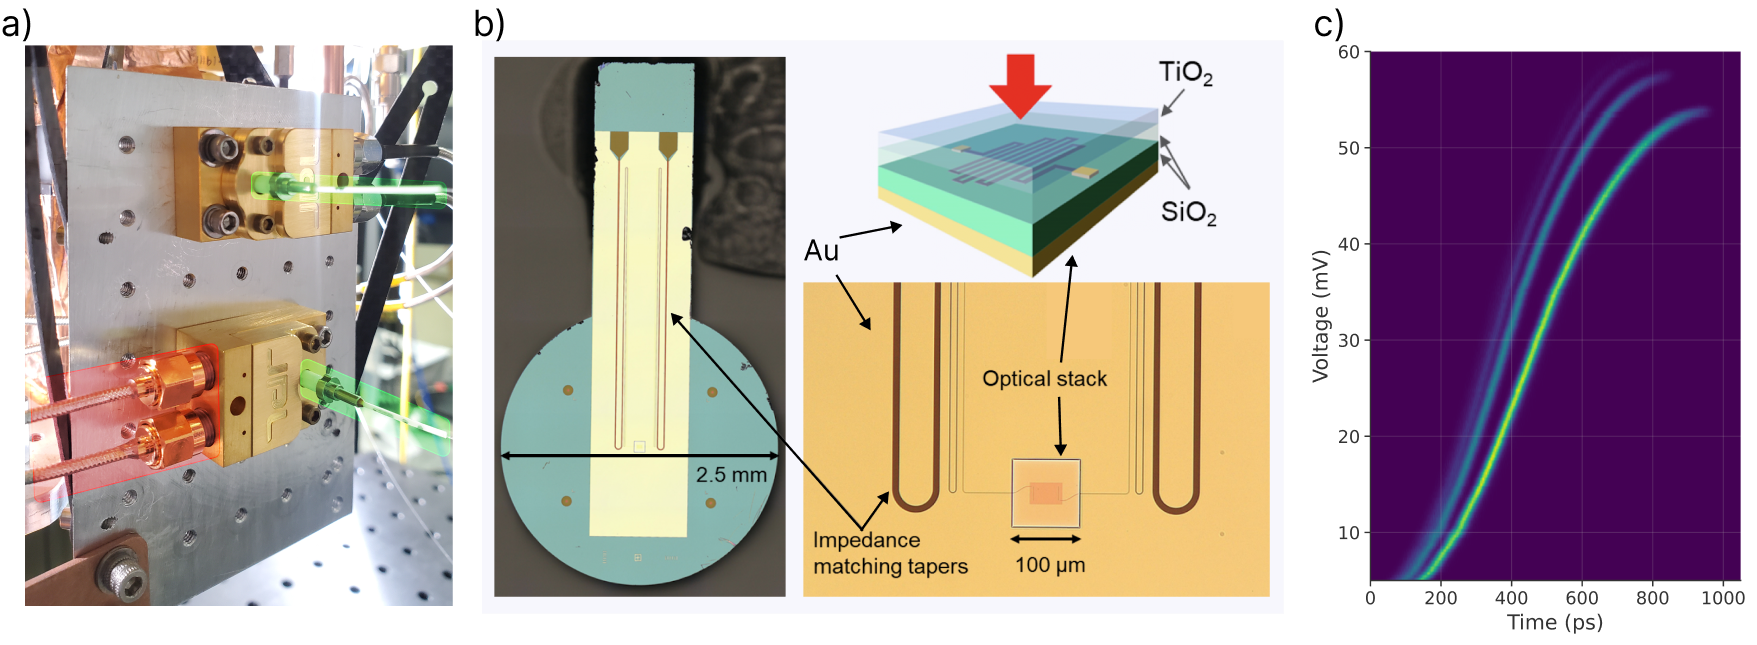
\includegraphics{./chapter_01/figs/diff_light.png}
\caption[{Differential Single Pixel}]{\textbf{Differential Single Pixel} a) Two packaged differential single pixel detectors. Coupled fibers highlighted in gree, differential SMA readout highlighted in red b) Magnified images of the detector lolipop-shape waver, highlighting where the tapers and efficiency-enhansing optical stack are located \textbf{\hl{image source?}} c) Integrated 2D histogram showing different heights and shapes of RF pulse rising edge in response to incident multi-photon optical pulses.}
\label{fig:diff}
\end{figure}
}

\hypertarget{geometric-jitter-cancellation-through-differential-readout}{%
\subsection{Geometric jitter cancellation through differential readout}\label{geometric-jitter-cancellation-through-differential-readout}}

Two main types of jitter arise in high efficiency SNSPD designs; amplifier jitter and geometric jitter. Amplifier jitter is where the readout electrical noise impacts the timing jitter, while geometric jitter emerges from the propagation delays created by detection events at various locations along the nanowire meander. Nanowires made of thin-film materials exhibit high kinetic inductance and behave like transmission lines with high characteristic impedance and slow phase velocity. These transmission line properties result in pulse propagation delays that contribute to the timing jitter of the detector. The arrival time of voltage pulses from the detector to time tagging equipment depends on the location of photon absorption in the nanowire, as detections closer to the ground termination and farther from the single readout must travel farther at low phase velocity through the nanowire before exiting. For large detectors, geometric jitter can contribute tens of picoseconds to the total system jitter. As detector size is often correlated with coupling efficiency to a given optical mode, the use of single-ended readout implies a trade-off between system detection efficiency and jitter due to longitudinal geometric effects.

The implementation of a differential readout approach offers a solution to these issues. Instead of just isolating the positive voltage pulse , the negative pulse from the other end of the nanowire is also collected. Simple processing of both pulses reveals information about photon arrival time as well as photon arrival location.

If the measurements of arrival time $t_F$ and absorption location along the nanowire are both of interest, then the timing of the $t_{neg}$ negative and positive $t_{pos}$ voltage pulses may be read out with 2 time taggers or high-speed oscilloscope channels. The difference of arrival time $t_{pos} - t_{neg}$ of these signals constitutes the photon absorption location information, while the average $1/2(t_{pos} - t_{neg})$ of the arrival times constitutes the photon arrival time information. For practical single photon counting applications, however, the photon arrival time information is typically sufficient and real-time processing of two time tags per detection event is not practical. Therefore, a 2:1 balun transformer can be used to perform an equivalent hardware difference of the complementary pulses (analogous to the averaging of timetags $t_{pos}, t_{neg}$). After amplification, the two sides of the detector are connected to the differential inputs of the balun, with the output being sent to a TCSPC or equivalent time tagging module. The threshold voltage of the time tagger can be set to minimize the spread of time tag distribution, corresponding to the condition where the timing measurement $t_{tagger} \approx t_F$ so that the photon arrival location information is cancelled out.

\hypertarget{increased-snr-with-impedance-matching-tapers}{%
\subsection{Increased SNR with impedance matching tapers}\label{increased-snr-with-impedance-matching-tapers}}

In a usual SNSPD, the nanowire exibits impedance on the order of $\mathrm{k} \Upomega$, while the readout circuit has an impedance of 50~$\Upomega$. This mismatch can lead to RF pulses that exhibit reflections and distortions. These effects reduce slew rate and and lower Signal to Noise Ratio, bringing about higher amplifier jitter~\autocite{Korzh2020,santavicca2019jitter}.

The higher jitter that results from the impedance mismatch can be mitigated by designing the SNSPD to preserve the integrity of the output pulse. An impedance-matching taper interfacing the nanowire to the readout line can be integrated. Thanks to the gradual impedance transformation of a Klopfenstein style taper, the output pulse has a higher amplitude and a faster slew rate. In a toy snspd model developed by Colangelo et al.~\autocite{Colangelo2023}, the incorporation of a taper increases pulse amplitude by a factor of 3.3.

Together the impedance matching tapers and differential readout work to reduce system jitter significant for large area meandered nanowires. For the research in this thesis, these detectors are usually used with a differencing balun for geometric jitter cancellation. The type fabricated at JPL typically have active areas of $22 \times 15 \ \mathrm{\upmu m}$, formed by a meander of 100 nm-wide and 5-nm-thick niobium nitride (NbN) nanowires on a 500 nm pitch (Fig.~\ref{fig:diff} b). They are embedded in an efficiency-enhancing optical stack made of alternating layers of TiO$_2$ and SiO$_2$ and a gold mirror layer and typically have FWHM timing jitter of about 14 ps. The FW1\%M jitter, which is a measure of the width of the jitter response function or histogram at 1\% height, is an important metric for quantum or classical communication protocols that expect to reliably place photon timing measurements into time bins measured with respect to a clock. This is the case for pulsed Quantum Key Distribution and classical Pulse Position Modulation communication protocols.

Also, the use of impedance matching tapers can help distinguish between instances when one or multiple photons are absorbed in the nanowire on a short timescale ($< 100~ps$). The absorption of different numbers of photons results in variations in RF pulse height and slew rate (Fig.~\ref{fig:diff} c). This phenomenon gives the detector photon number resolution (PNR) whereby the specific number of photons in a optical pulse can be measured. This is in contrast to the more common binary detection capability offered by conventional SNSPDs that only indicates if one or more photons are absorbed. Chapter 4 explores how the manifestation of photon number resolution in this detector type presents a problem for accurate time correlated measurements of multi-photon light pulses.

\textbf{\hl{TODO structure of this thesis here}}

\hypertarget{low-dark-count-rate-detection}{%
\chapter{Low Dark Count Rate Detection}\label{low-dark-count-rate-detection}}

The work described in this chapter culminated in the research paper: Andrew S. Mueller, Boris Korzh, Marcus Runyan, Emma E. Wollman, Andrew D. Beyer, Jason P. Allmaras, Angel E. Velasco, Ioana Craiciu, Bruce Bumble, Ryan M. Briggs, Lautaro Narvaez, Cristián Peña, Maria Spiropulu, and Matthew D. Shaw, ``Free-space coupled superconducting nanowire single-photon detector with low dark counts,'' \href{https://opg.optica.org/optica/fulltext.cfm?uri=optica-8-12-1586\&id=465726}{Optica 8, 1586-1587 (2021)}

Boriz Korzh provided extensive assistance during ideation, construction, testing, and copyediting phases of the experiment. Bruce Bumble designed the elevated 0.8 K stage and innovated translation system using flexible carbon fiber rods. Jason Trevor provided technical assistance with the implementation of a nitrogen flow bag. Sahil Patel assisted with editing the manuscript.

\hypertarget{abstract}{%
\section{Abstract}\label{abstract}}

\emph{A free-space coupled superconducting nanowire single photon detector with high efficiency at 1550 nm, sub-0.1 Hz dark count rate, and sub-15 ps timing jitter is demonstrated.}

\hypertarget{background}{%
\subsubsection{Background}\label{background}}

Superconducting nanowire single photon detectors are high sensitive devices. Any stray photons from a laboratory environment can make their way into these devices and produce a detection. These detections are commonly called dark counts or false counts. Dark counts can be present in any situation where the detector is coupled to some experiment or apparatus outside the cryogenic environment. This coupling may be through windows inside the cryostat housing and radiations shields, or through optical fibers that carry single-mode signals directly to detectors.

Visible, near-infrared, and mid-infrared photons are often the main sources of dark counts, because they are ubiquitous in a laboratory environment and are transmitted through common types of fibers and windows. Assuming visible light can be blocked from entering the detector system, the blackbody emission of the room temperature laboratory environment presents is the primary source of dark counts. The spectrum of blackbody photons, defined by Planck's law, is peaked at about $10~\mathrm{\upmu m}$, though it can contribute dark counts at significant rates up through near-infrared wavelengths.

Without filtering in fiber or free space, dark counts from blackbody emission will overload most SNSPDs and overpower the extremely faint signal of interest. In this work we investigate minimize dark counts through the use of cryogenic free space filtering.

\textbf{\hl{more here}}

\hypertarget{introduction-1}{%
\section{Introduction}\label{introduction-1}}

Time-resolved photon detection with low dark counts is a vital technology in fields such as quantum information processing, classical communication, quantum communication, and laser ranging. Increasingly, research in these fields employs superconducting nanowire single photon detectors (SNSPDs), which have been demonstrated with system detection efficiency ($\eta$) of more than 90\% \autocite{Reddy2020}, timing jitter ($\Delta t$) as low as 2.6 ps \autocite{Korzh2020} and intrinsic dark count rates ($D$) in the milli- to micro-hertz range \autocite{Hochberg2019}. However, quantum communication applications require detection systems with performance optimized across all three metrics simultaneously. The dimensionless figure of merit $H$ specifies this application-specific performance as $H = \frac{\eta}{(\Delta t D)}$~\autocite{Hadfield2009}.

Here, we focus on lowering the Dark Count Rate (DCR) of a telecom-band SNSPD system by filtering thermal photons, without sacrificing efficiency or jitter. We demonstrate a free-space coupled SNSPD with sub-0.1 Hz DCR, 14 ps timing jitter, and 72\% total system detection efficiency (SDE) by using a differential single-pixel SNSPD \autocite{Colangelo2021} to image a single-mode fiber through an optimized free-space filter stack.

The highest system detection efficiencies have been achieved using self-aligned fiber coupling where dark counts can be reduced using cryogenic fiber looping \autocite{Cohen2015} or spliced narrow-band filters \autocite{Boaron2018secure}. But it is difficult to achieve strong filtering without losses at the target wavelength. Low-loss, high-rejection filters are typically available as free-space components, so some of the highest reported H-values were achieved with cryogenic, fiber to free-space to fiber coupling, but exhibit an SDE of only a few percent \autocite{Shibata2015}. The filtering method presented here takes advantage of commercially-available filters, achieves a high free-space coupling efficiency using a cryogenic lens, and is compatible with both fiber and free-space optical inputs.

In this work, a single mode fiber is imaged onto the detector using two f = 18.75 mm lenses. One lens collimates light from an optical fiber face outside the cryostat (Photon Spot), and the other focuses light onto the detector inside \autocite{Bellei:16}. In the collimated region between, the beam passes though a series of short-pass filters and one band-pass filter mounted at 4 K ( Fig.~\ref{fig:setup} a). One of the short-pass filters is angled to avoid ghosting effects. The 40 K radiation shield and outer cryostat housing are fitted with anti-reflection coated BK7 windows. The filters are spring loaded to prevent cracking at low temperatures. To minimize effects of stray light, the interior of the 4 K shield was painted with mid-IR absorbing paint (Aeroglaze Z306) \autocite{Persky1999}, while gaps between filters and the windows were covered with metal tape.

The system is based on 1-inch optics, although the f = 18.75 mm lenses lead to a $1/e^2$ intensity diameter of about 5 mm in the collimated region. To reduce the larger-than-required numerical aperture of the system, painted 8 mm apertures (Acktar Spectral Black) were added in the collimated region. These are large enough to allow minor alignment adjustments --- by translating the exterior collimating lens --- without vignetting.

We use four custom cryogenic short-pass filters, with pass-bands below $1.6 \ \mathrm{\upmu m}$ and $1.9 \ \mathrm{\upmu m}$ (Andover Corp.), both with transmission at 1550 nm of 98.8 ± 0.3\%. They reject wavelengths shorter than $3 \ \mathrm{\upmu m}$ through reflective optical coatings, and attenuate longer wavelengths through material absorption in the 12.7 mm-thick N-BK7 glass substrate. While the bandpass filter (FWHM = 7 nm) was found to blue-shift by about 2 nm at cryogenic temperatures, the passband was wide enough such that significant attenuation was not observed at the original target wavelength of 1550 nm. This filter is also sufficiently wide to avoid Fourier-limited broadening of ultra-short laser pulses.

The filtering of the optical stack was modeled by assuming a black-body emitter at 298 K and a field of view defined by the 18.75 mm focal length of the cryogenic lens and the 8 mm diameter of the apertures. The resulting spectrum was multiplied by the transmission of the filters ( Fig.~\ref{fig:setup} b) and detector optical stack ( Fig.~\ref{fig:setup} c). The model showed that two each of the $1.6 \ \mathrm{\upmu m}$ and $1.9 \ \mathrm{\upmu m}$ short pass filters were necessary to suppress mid-infrared light to where it was no longer the dominant source of dark counts. With the inclusion of the four shortpass filters, the dominant source of dark counts is the spectral region near 1550 nm as shown in Fig.~\ref{fig:false-color} a, which also illustrates the effect of the bandpass filter. Also evident in Fig.~\ref{fig:false-color} a is the strong dependence of DCR on the temperature of the final surface outside the cryostat emitting thermal radiation. This motivated the exterior cooling apparatus shown at the bottom of Fig.~\ref{fig:setup} a. The bulkhead holding the fiber connector is cooled to around -2$^\circ$C using a Peltier element and liquid cooling block. This addition reduced the system DCR from 0.4 Hz to below 0.1 Hz. While dark counts from multiple spatial modes are present in this system --- modes that would not be present in a purely fiber based approach --- the external cooling technique works to minimize their effect.

This work used a low-jitter, differential SNSPD \autocite{Colangelo2023}, with an active area of $22 \times 15 \ \mathrm{\upmu m}$, formed by a meander of 100 nm-wide and 5-nm-thick niobium nitride (NbN) nanowires on a 500 nm pitch. A more conventional single-ended readout SNSPD of similar area would also achieve low DCR in this coupling system, but would likely achieve a lower performance metric $H$ from correspondingly higher jitter. The nanowire is embedded in an efficiency-enhancing optical stack made of alternating layers of TiO$_2$ and SiO$_2$ and a gold mirror layer. As shown in Fig.~\ref{fig:false-color} b and c, when fiber coupled (without any fiber-based filtering methods applied), this detector achieved a saturated SDE of $84\% \pm 4.4 \%$ and a DCR of 20 Hz at a bias current of $16\ \mathrm{\upmu A}$.

~~~~~ As also shown in Fig.~\ref{fig:false-color} b, the free-space coupling system achieves up to $72 \% \pm 3.7 \%$ SDE as measured from the fiber outside the cryostat. The reduction in efficiency is likely due to surface reflections in the free-space optics, and potential misalignment in the optical baffles. The minimum DCR ( Fig.~\ref{fig:false-color} c) at $72 \%$ SDE is about 0.1 Hz, with a bias current of 16 $\mathrm{\upmu A}$. These metrics, with the jitter measurements shown in Fig.~\ref{fig:false-color} b, give a maximum H value of $5 \times 10^{11}$ ( Fig.~\ref{fig:false-color} c). Values as high as $1.8 \times 10^{12}$ have been reported before, but at 1.5\% system detection efficiency \autocite{Shibata2015}. Our system shows a low DCR can be achieved without severe reduction of SDE or usable target wavelength bandwidth. This is paramount for the future of terrestrial and space-to-ground quantum communication, since it increases success rate with finite statistics \autocite{Boaron2018secure}. The same techniques can be applied to emerging SNSPD applications at longer wavelengths, such as laser ranging \autocite{Taylor2019}, where fiber filtering is impractical. Beyond single-mode applications, our work paves the way to scalable, low-DCR, multi-mode coupling to SNSPD arrays \autocite{Wollman2019}.

\hypertarget{optical-alignment-setup}{%
\section{Optical Alignment Setup}\label{optical-alignment-setup}}

\textbf{\hl{TODO}}

\hypertarget{time-walk-and-jitter-correction}{%
\chapter{Time Walk and Jitter Correction}\label{time-walk-and-jitter-correction}}

A version of this chapter is currently published as:

Andrew Mueller, Emma E. Wollman, Boris Korzh, Andrew D. Beyer, Lautaro Narvaez, Ryan Rogalin, Maria Spiropulu, Matthew D. Shaw; \href{https://pubs.aip.org/aip/apl/article/122/4/044001/2870246/Time-walk-and-jitter-correction-in-SNSPDs-at-high}{Time-walk and jitter correction in SNSPDs at high count rates}. Appl. Phys. Lett. 23 January 2023; 122 (4): 044001.

Portions of this chapter appear in:

Ioana Craiciu, Boris Korzh, Andrew D. Beyer, Andrew Mueller, Jason P. Allmaras, Lautaro Narváez, Maria Spiropulu, Bruce Bumble, Thomas Lehner, Emma E. Wollman, \& Matthew D. Shaw (2023). \href{https://opg.optica.org/optica/fulltext.cfm?uri=optica-10-2-183\&id=525546}{High-speed detection of 1550 nm single photons with superconducting nanowire detectors}. Optica, 10(2), 183--190.

\hypertarget{abstract-1}{%
\section{Abstract}\label{abstract-1}}

~~~~~

Superconducting nanowire single-photon detectors (SNSPDs) are a leading detector type for time correlated single photon counting, especially in the near-infrared. When operated at high count rates, SNSPDs exhibit increased timing jitter caused by internal device properties and features of the RF amplification chain. Variations in RF pulse height and shape lead to variations in the latency of timing measurements. To compensate for this, we demonstrate a calibration method that correlates delays in detection events with the time elapsed between pulses. The increase in jitter at high rates can be largely canceled in software by applying corrections derived from the calibration process. We demonstrate our method with a single-pixel tungsten silicide SNSPD and show it decreases high count rate jitter. The technique is especially effective at removing a long tail that appears in the instrument response function at high count rates. At a count rate of 11.4 MCounts/s, we reduce the full width at 1\% maximum level (FW1\%M) by 45\%. The method, therefore, enables certain quantum communication protocols that are rate-limited by the FW1\%M metric to operate almost twice as fast.

\hypertarget{introduction-2}{%
\section{Introduction}\label{introduction-2}}

\hypertarget{origin-of-time-walk}{%
\subsection{Origin of time walk}\label{origin-of-time-walk}}

Over the last decade, SNSPDs have advanced rapidly to become essential components in many optical systems and technologies, owing to their high efficiency $(>90\%)$~\autocite{99.5_Chang_2021,reddy2020superconducting}, fast reset times ($< 1~\mathrm{ns}$)~\autocite{Vetter2016Cavity} and scalability to kilopixel arrays~\autocite{Wollman2019}. The timing jitter of SNSPDs is also best-in-class -- values as low as 3~ps have been demonstrated in short nanowires~\autocite{Korzh2020}, and new high-efficiency designs exhibit sub-10 ps jitter~\autocite{EsmaeilZadeh2020,Colangelo2021}.

SNSPD jitter increases with count rate due to properties of the nanowire reset process and features of the readout circuit. The effect bears resemblance to time walk observed in silicon avalanche diodes and other detectors where the pulses have varying heights and slew rates~\autocite{SPAD_walk_Kirchnir_1997} thereby causing a timing measurement using a fixed threshold to `walk' along the rising edge of the pulse (the labeled delay in Fig.~\ref{fig:jitterate_intro} a).
At low count rates SNSPDs exhibit very uniform pulse heights. However, at high counts rates where the inter-arrival time is on the order of the reset time of the detector, current-reset and amplifier effects lead to smaller and distorted pulses. If photon inter-arrival times are not known a priori in the intended application, the uncorrected time walk manifests as a perceived increase in jitter (Fig.~\ref{fig:jitterate_intro} b).

\hypertarget{fig:jitterate_intro}{%
\begin{figure}
\centering
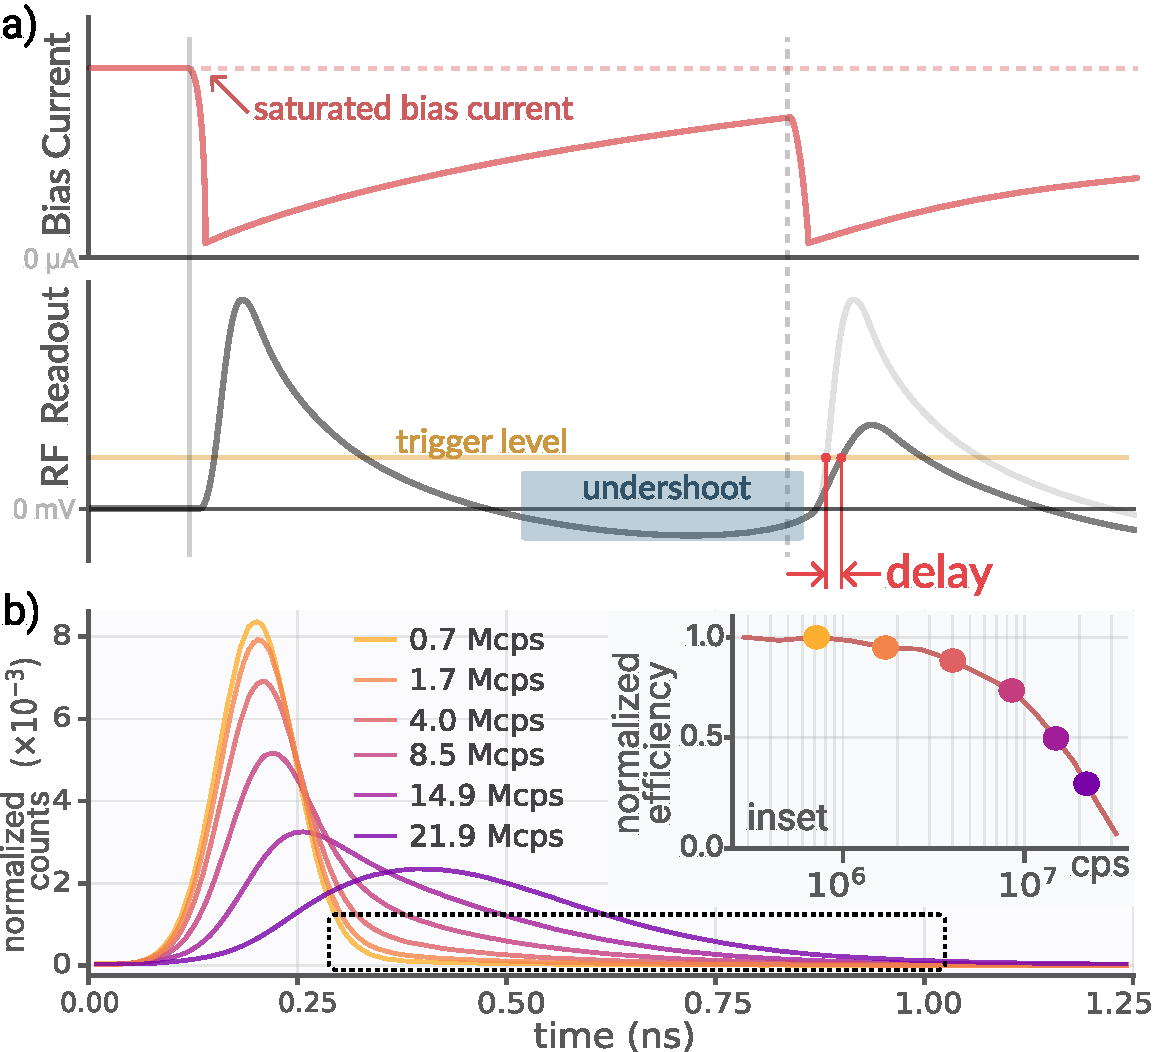
\includegraphics[width=0.7\textwidth,height=\textheight]{./chapter_03/figs/intro_jitterate_light.pdf}
\caption[{Introduction to the time walk effect}]{\textbf{Introduction to the time walk effect} a) Diagram illustrating two major sources of correlated high count rate jitter. First, detections may occur during the reset time of a previous detection. At this time the bias current in the nanowire is below its saturated value so that a photodetection triggers an RF pulse with correspondingly lower amplitude. Second, an RF pulse may arrive in the undershoot region of a previous pulse, where the undershoot is a period of negative voltage induced by the low-frequency cutoff properties of the readout amplifier chain. (b) Measured histograms of detections from short $3~\mathrm{ps}$ mode-locked laser pulses. With lower attenuation and higher count rate, the observed timing uncertainty is greater. Inset shows where respective count rates fall on a maximum count rate (MCR) curve \autocite{Zhang_MCR_2019}. The MCR of an SNSPD is often quoted at the $3~\mathrm{dB}$ point, where the normalized efficiency drops to $-3~\mathrm{dB}$ of its maximum value. The jitter increase due to time walk manifests as a tail in the instrument response functions (inside dashed black box) even at count rates significantly below the 3-dB point where detector efficiency has not started to drop significantly (e.g.~the 1.7 Mcps data)}
\label{fig:jitterate_intro}
\end{figure}
}

The time-walk effect in SNSPDs is typically not reported, as jitter is usually measured at low count rates where the detector has ample time to reset following each detection. But as communication and quantum information applications push into higher count rates, the high count rate induced jitter becomes more relevant. LIDAR, quantum and classical optical communication, and imaging applications may all benefit from the development of new detection systems and methods that keep jitter as low as possible in this regime.

We first consider the features of SNSPD operation and readout that cause an increase in jitter with count rate. Then we present multiple ways of mitigating or avoiding these effects, before reviewing our preferred method that relies on a calibration and correction process.

The jitter increase observed at high rate originates from two groups of system characteristics: (i) the intrinsic reset properties of the nanowire, and (ii) properties of the amplification chain. These influence the system's jitter differently, thus it is helpful to consider them separately. Added jitter from either or both sources can emerge when an SNSPD system is operated at high count rates.

The nanowire reset process determines how the detector becomes single-photon sensitive again after a detection. When an SNSPD fires, the current flow in the nanowire momentarily drops to near zero, then recovers in an inverted exponential fashion (Fig.~\ref{fig:jitterate_intro} a). An incident photon may trigger another detection before the bias current fully returns to its saturated value, producing a pulse with a lower amplitude and slew rate. A fixed threshold comparator will trigger on this lower pulse later in time than a full amplitude pulse. If uncorrected for, this time walk manifests as an increase in jitter at high count rates.

The choice of readout amplifiers may also contribute to added high count rate jitter. Pulses may be shifted in voltage and distorted if they arrive when the RF signal has not yet reached a steady zero state following the previous detection. For example, pulses may arrive within an amplifier-induced undershoot region following previous pulses. This phenomenon is illustrated in Fig.~\ref{fig:jitterate_intro} a as the area below 0~mV. The duration of ringing or undershoot effects varies widely depending on the design of the readout circuit. If they last longer than the reset time of the nanowire bias current, the calibration technique may correct for the potentially complex interactions between pulse waveforms that overlap in time.

\hypertarget{jitter-mitigation-methods-at-high-count-rates}{%
\subsection{Jitter Mitigation Methods at High Count Rates}\label{jitter-mitigation-methods-at-high-count-rates}}

There are various methods for correcting for increased jitter at high count rates. These include (i) the use of extra hardware that cancels out some distortions, or (ii) simple software-based data filtering that ignores distorted time-tags. We review these techniques before covering the calibration and correction approach.

Variations in pulse height are a primary component of the distortions that appear at high rates. Such variations in other systems are commonly corrected with a constant fraction discriminator (CFD) that allows for triggering at a fixed percentage of pulse height rather than at a fixed voltage. Adding a CFD to an existing setup is straightforward for a single channel, however it does require additional hardware such as multiple high-speed discriminators and a D-type flip-flop~\autocite{Becker2005}, which significantly increases the circuit complexity and power budget of a multi-channel system. In addition, CFDs are not expected to optimally correct for distortions of the pulse rising edge which may arise from the overlap of one pulse with a signal reflection or undershoot features on the falling edge of a previous pulse. Multi-channel time-to-digital converters (TDCs) used to read out large SNSPD arrays typically only include fixed-threshold comparators~\autocite{Wollman2019}.

In a simple software-based jitter mitigation method, each time-tagged event may be accepted or rejected based on how soon it arrives after the previous pulse. Those that arrive within some pre-determined dead time are assumed to be corrupted by pulse distortions. These are rejected, and the rest are accepted. This method can lower system jitter and maintain high data rates, especially in the cases where only a few percent of pulses are filtered out. However, it can severely limit count rate near the $3~\mathrm{dB}$ point where the majority of counts are rejected (see the supplementary material).

Our correction method preserves original count rate and works with timing measurements from a fixed-threshold free-running TDC -- the type that is often used for SNSPD readout. Pulse pileup correction techniques have been demonstrated with systems that fully digitize detector pulse waveforms~\autocite{Behbahani2019,scoullar_evans_2009,Haselman2010}. But capturing the fast rising edges of SNSPD pulses in this way would require very high sample rates and subsequently, impractically large data streams. In contrast, our method assumes one timing measurement is acquired from triggering on the rising edge of each SNSPD pulse.

We calculate the time between a given \emph{current} SNSPD detection event and a preceding event. This inter-arrival time is used to determine a timing correction for the current event using a lookup table. A calibration routine described next is needed to build this lookup table. Applying these corrections during real-time processing removes deterministic delays correlated with the time between time-tags, leaving only stochastic jitter.

\hypertarget{method-and-results}{%
\section{Method and Results}\label{method-and-results}}

\hypertarget{experimental-setup}{%
\subsection{Experimental setup}\label{experimental-setup}}

The measurements used for calibration and correction were acquired with a high rate mode locked laser (\emph{Pritel}). The minimum repetition rate of this laser was too high to produce a calibration dataset for the Tungsten Silicide detector at highest count rate, given the constraints addressed in the main text. Therefore, the laser was set at a repetition rate of 10.75 GHz and modulated down to 537.5 MHz using two lithium niobate intensity modulators in series. Residual peaks from suppressed mode-locked laser pulses are not observed above the noise floor in the collected data, so their effect was not further considered. Clock jitter is minimized in post-processing with the help of a software-based Phase Locked Loop.

\hypertarget{fig:jitterate_exp_setup}{%
\begin{figure}
\centering
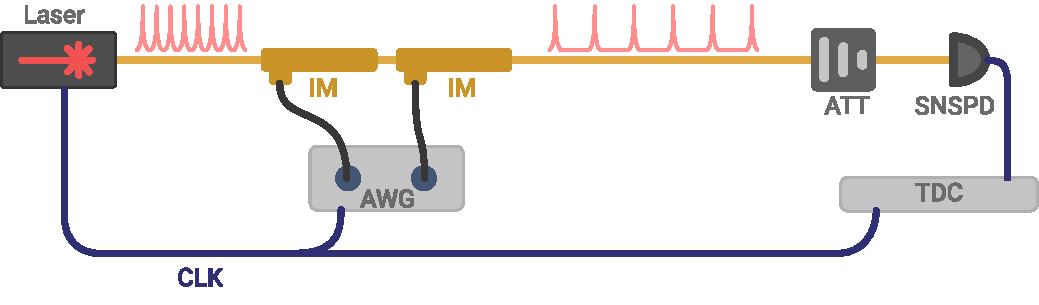
\includegraphics[width=0.9\textwidth,height=\textheight]{./chapter_03/figs/supplemental_expirement_light.pdf}
\caption[{Time walk experiment setup}]{\textbf{Experimental Setup} CLK: clock synchronization signal; AWG: Arbitrary Waveform Generator (\emph{Keysight}); IM: Intensity Modulator (\emph{IXBlue}); TDC: Time to Digital Converter (\emph{Swabian Instruments}). The extinction ratio of both modulators exceeds 30 dB.}
\label{fig:jitterate_exp_setup}
\end{figure}
}

\hypertarget{detector-and-trigger-level}{%
\subsection{Detector and trigger level}\label{detector-and-trigger-level}}

We study the pulse distortions observed in a fiber coupled single-pixel tungsten silicide (WSi) SNSPD with 380~$\mathrm{\upmu m^2}$ active area and 160~nm nanowire width. The detector is biased at 9.3~$\mathrm{\upmu A}$, roughly 90\% of the switching current. The readout is handled by a cryogenic DC-coupled amplifier, mounted on the 40~K-stage of the cryostat, which has 43~dB of gain and a 3~dB bandwidth of 700 MHz, followed by a 1~GHz amplifier with 20~dB of gain (\emph{MiniCircuits ZFL-1000LN+}). The system reaches a $3~\mathrm{dB}$ maximum count rate (MCR) of $15.6~\mathrm{MHz}$. The time constant of supercurrent recovery $\tau_{bias} \approx 40~\mathrm{ns}$ is significantly longer than the decay time constant of the RF pulse $\tau_{RF} \approx 5~\mathrm{ns}$, owing to our use of a low-frequency cut-on of $\approx 80$~MHz (-3~dB point from the peak gain) in the DC-coupled amplifiers. For this detector, the calibration process primarily corrects for the lower bias current effects, rather than for any overlapping between RF pulse waveforms (see \textbf{\hl{supplementary material}}). Other detector types and readout systems may operate in a different regime.

The jitter increase with count rate is highly dependent on trigger level. High rate distortions affect the timing measurements less if the threshold voltage is set just above the noise floor.
But triggering on the pulse higher, where it achieves maximum slope, minimizes jitter at low-to-medium count rates. This level varies from 20\% to 50\% of pulse height depending on the detector. We found the minimum low-rate jitter at a trigger level of 50~mV, about 40\% of the pulse height. All further calibration and analysis is performed by triggering at this level in order to optimize jitter across all count rates.

\hypertarget{mode-locked-laser-calibration}{%
\subsection{Mode locked laser calibration}\label{mode-locked-laser-calibration}}

To perform our calibration, we illuminated the SNSPD with an attenuated 537.5~MHz mode locked laser with a mean photon number per pulse between $5\mathrm{e}{-4}$ and $0.016$. The 1.86~ns period of the pulse sequence is large enough that almost all SNSPD detections can be unambiguously matched with a preceding laser pulse -- the period of the pulse train used must be greater than the worst detector jitter for this to succeed. The uncorrected jitter for the WSi detector varies from 50~ps FWHM at low count rates, to about 350~ps at high rates.

\hypertarget{fig:jitterate_explain}{%
\begin{figure}
\centering
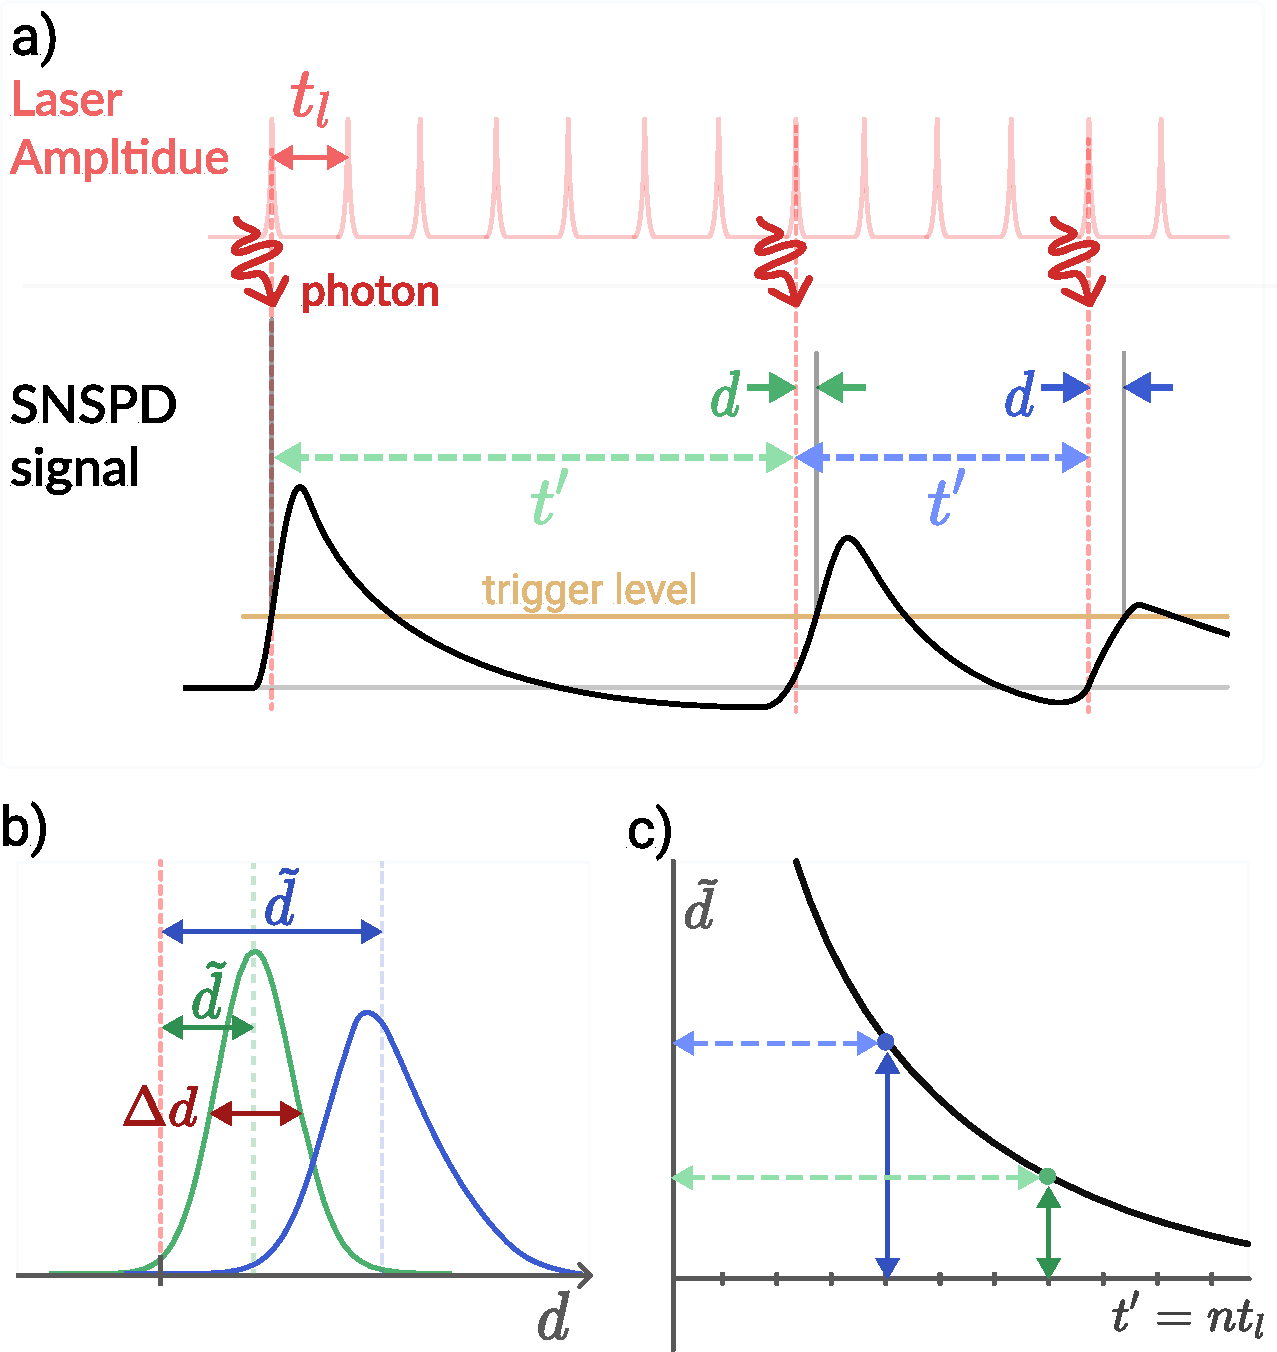
\includegraphics[width=0.7\textwidth,height=\textheight]{./chapter_03/figs/jitterate_explain_light.pdf}
\caption[{Calibration method for extracing t' vs delay}]{\textbf{Calibration Method} a) A qualitative diagram illustrating how inter-pulse timing measurements $t'$ and $d$ are extracted. A small fraction of laser pulses contain a photon due to the low mean photon number per pulse of the attenuated laser. Pairs of subsequent photon arrivals are separated by a time denoted by $t' = n t_l$. b) Possible distributions of delay $d$ measurements for two different $t'$. The median of these defines the extracted delay parameters $\tilde{d}$ which form the y-axis in the calibration curve illustrated in (c). The $\tilde{d}$ vs $t^\prime$ curve in (c) approaches zero for $t^\prime$ approaching infinity. Blue and green arrows with matching color and style denote the same measure in (a), (b), and (c).}
\label{fig:jitterate_explain}
\end{figure}
}

We collect sorted time-tags and first consider adjacent pairs of SNSPD events as illustrated in Fig.~\ref{fig:jitterate_explain} a. The time between the two photons that produced these event pairs is defined as $t^\prime$, which is an integer number of laser periods ($t^\prime = n t_{l}$). Second, we derive the delay between the second event and its corresponding laser pulse, defined as $d$. For each laser period spacing $t^\prime$, we make a histogram of the second event delays and find the median ($\tilde{d}$) and the FWHM ($\Delta {d}$) of this distribution. For shorter separations $t^\prime$, the distribution is expected to have larger delays and FWHM (Fig.~\ref{fig:jitterate_explain} b) due to the smaller pulse height of the second event. Finally, we use the median delay as a function of laser spacing (Fig.~\ref{fig:jitterate_explain} c) to form a curve $\tilde{d}$-vs-$t^\prime$ for the added time-walk versus inter-arrival time.

\hypertarget{fig:jitterate_results_1}{%
\begin{figure}
\centering
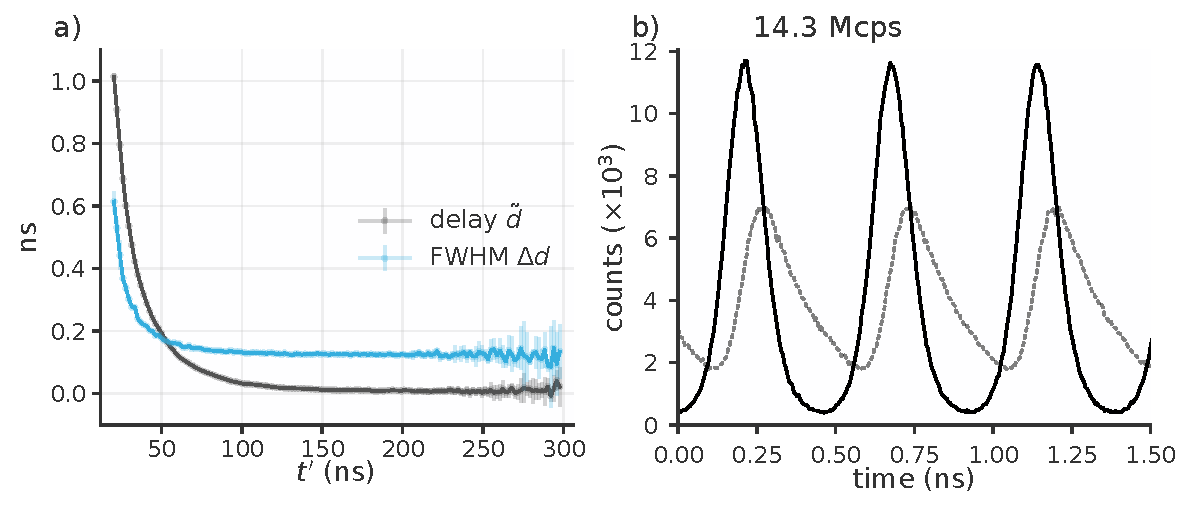
\includegraphics[width=0.9\textwidth,height=\textheight]{./chapter_03/figs/jitterate_data_ab_light.pdf}
\caption[{t-prime curve and correction effect}]{\textbf{t-prime curve and correction effect} (a) Delay and intrinsic jitter curves extracted from the 537.5 MHz pulsed light dataset. (b) Histogram of corrected (black) and uncorrected (dashed grey) time tags from a 2.15 GHz pulse train, corrected using a calibration curve developed with the 537.5 MHz dataset. The improvement affirms that the light modulation used for an application need not match the repetition rate of the calibration laser.}
\label{fig:jitterate_results_1}
\end{figure}
}

Fig.~\ref{fig:jitterate_results_1} a shows the $\tilde{d}$-vs-$t^\prime$ and $\Delta d$-vs-$t^\prime$ curves collected from our measurements of the WSi detector. The $\tilde{d}$-vs-$t^\prime$ curve is the main result of the calibration process and is used as a lookup table in the correction method. $\Delta d$ is a measure of the more intrinsic jitter that the correction method cannot cancel out. While it is larger for small $t^\prime$ due to triggers on lower amplitude pulses, it notably stays at a nearly minimized value down to around $t^\prime =$ 50~ns. $\tilde{d}$ grows more dramatically with decreasing $t^\prime$, especially in the range from 50~ to 100~ns. For count rates that don't exhibit many inter-pulse arrival times smaller than 50~ns, a method for removing the time-walk effect's contribution to jitter should bring entire system jitter back down to near the intrinsic limit implied by the $\Delta d$ curve.

The correction method we implement involves subtracting off the distortion-induced delays a time-tag is expected to have based on the inter-pulse-time that precedes it. For each time tag $t_n$ in a set, the inter-pulse time is $t_n - t_{n-1} = \Delta t$, where $t_{n-1}$ is the previous tag on the same channel. Using $\Delta t$ as an index, a corresponding delay correction $\hat{d}$ is found by interpolating the $\tilde{d}$-vs-$t^\prime$ curve from the calibration. Given the density of points in the $\tilde{d}$-vs-$t^\prime$ acquired here, a linear interpolation is sufficient. The correction may benefit from higher order interpolation if the $\tilde{d}$-vs-$t^\prime$ curve is more sparse. This would be the case for calibrations built from a slower repetition rate pulsed light source. An assumption underlying the correction is that the interpolated value $\hat{d}$ is a good estimator of the true delay added to the current time-tag due to high count rate pulse distortions.

With the interpolation operation expressed as a function $D$, the correction is written as $\overline{t}_n = t_n - D(\Delta t)$, where $\overline{t}_n$ is the corrected version of tag $t_n$. Whether $t_{n-1}$ is itself corrected or uncorrected has negligible influence on the $t_n$ correction, as we assume $d << \Delta t$. The data correction shown here was applied in post-processing. But since $D$ depends only on the current time tag and information available from earlier, the correction can be applied in real-time in an FPGA or computer used for time tagging.

\hypertarget{fig:jitterate_results_2}{%
\begin{figure}
\centering
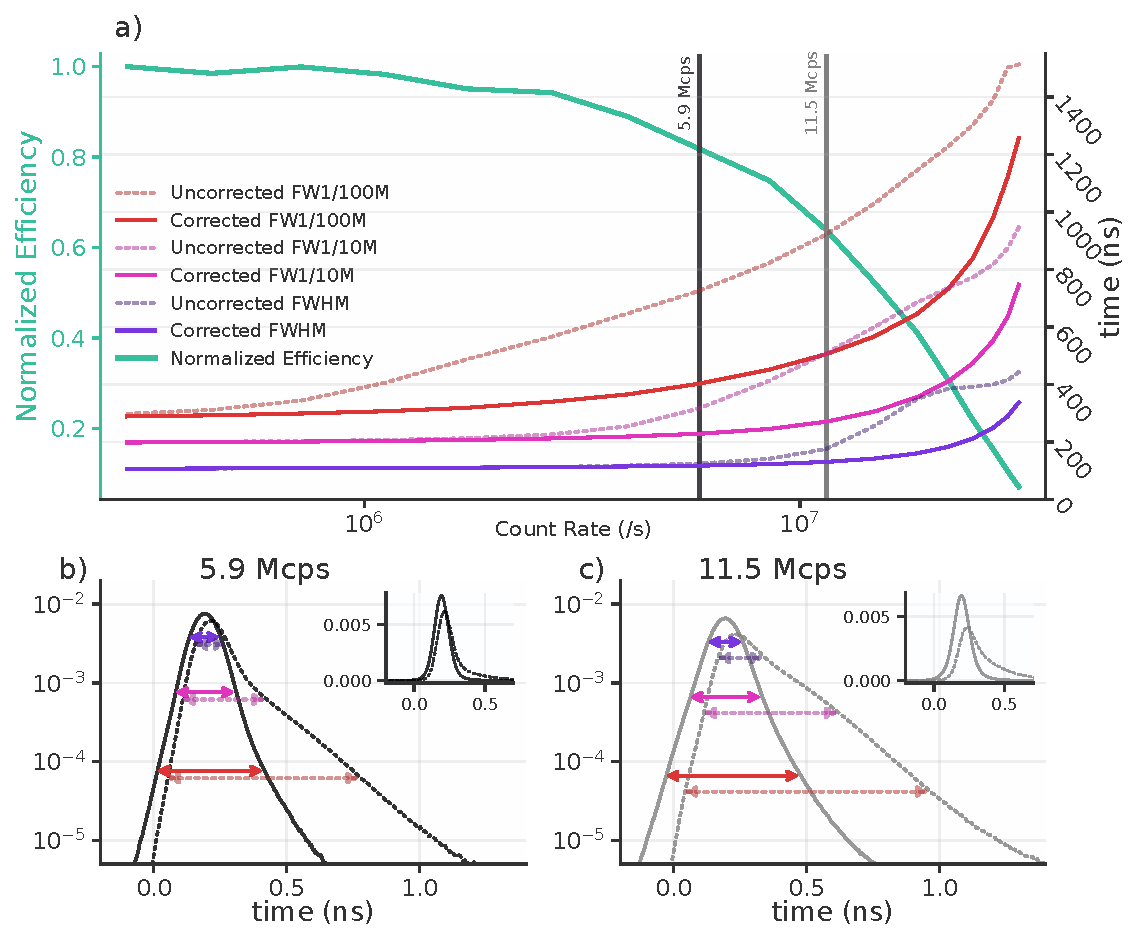
\includegraphics[width=0.9\textwidth,height=\textheight]{./chapter_03/figs/jitterate_data_c_light.pdf}
\caption[{Jitters metrics across incident powers}]{\textbf{Jitters metrics across incident powers} (a) Effect of the correction on measurements of system jitter over a range of rates approaching the maximum count rate. (b) Corrected (solid) and uncorrected (dashed) instrument response functions with color-matched arrows showing the location of the width-statistics plotted above in (a). The black vertical line in (a) is drawn at the count rate of this plot. Inset shows linear scaling. (c) Corrected (solid) and uncorrected (dashed) histogram analogous to (b), but at a higher count rate indicated by the grey line in (a).}
\label{fig:jitterate_results_2}
\end{figure}
}

The correction we perform using the $\tilde{d}$-vs-$t^\prime$ curve in Fig.~\ref{fig:jitterate_results_1} a is applicable to a wide range of count rates and arbitrary modulation patterns; there is no requirement that applications match the repetition rate of the calibration laser. Fig.~\ref{fig:jitterate_results_1} b shows that the correction method, derived from the 537.5 MHz calibration data, significantly reduces jitter when applied to detections from a 2.15~GHz pulse train. A similar jitter reduction can be demonstrated for repetition rates below 537.5~MHz.

To study the effectiveness of our correction method at different count rates, we apply it to data collected at different mean photon numbers per pulse, with the same 537.5 MHz pulse train. As shown in Fig.~\ref{fig:jitterate_results_2} c, the correction improves the FWHM at rates approaching the 3~dB point, and improves FW10\%M and FW1\%M (full width at ten percent/one percent maximum) dramatically, even at count rates significantly below the 3 dB point, where detector efficiency is nearly maximized. This reduction is evident in Fig.~\ref{fig:jitterate_results_2} c, where the correction works to remove a time-walk induced tail in the instrument response function. The ratio of corrected FW1\%M over uncorrected FW1\%M reaches a minimum of 0.55 at a count rate of 11.5 MCounts/s. Therefore if an application sets its repetition rate or bin size based on the FW1\%M metric, the repetition rate can be increased and the bin size decreased by up to 45\% without any increase in event misattribution errors. These improvements are notable for applications including biomedical imaging~\autocite{Sutin16,Bruschini2019}, quantum communication~\autocite{Hadfield2009} and laser ranging~\autocite{McCarthy13} that have stringent timing requirements over a large dynamic range.

\hypertarget{higher-order-correction-the-peacoq-detector}{%
\section{Higher order correction \& the PEACOQ detector}\label{higher-order-correction-the-peacoq-detector}}

The Performance Enhanced Array for Counting Optical Quanta (PEACOQ) is a new fiber-coupled SNSPD design that achieves high count rate by spreading the photon flux across a parallel array of short niobium nitride nanowires. Each wire may acheive count rates as high as 50 MCounts/s, so the 32-wire array as a whole can handle photon rates in excess of 1 GCounts/s. The PEACOQ is described in detail in Reference \autocite{Craiciu23}.

From early tests of the PEACOQ, it became evident that jitter increased dramatically at high single wire count rates. One of the overaching goals the the PEACOQ project was to demonstrate near-100~ps jitter at 1 GCount/s. Therefore, we investigated the possibility of applying time walk correction techniques to this detector. This began with collecting a calibration dataset like that discussed in section \ref{mode-locked-laser-calibration}.

A 1-GHz repetition rate 1550 nm mode locked laser was used (Pritel UOC) for calibration. The 1~GHz repetition rate was chosen so that uncorrected jitter even at the highest count rates (approaching 400 ps at the FW1\%M), was smaller than the laser period. Then, each time tag may be matched to the timing of the original optical pulse. A dataset with a count rate of 20 MCounts/s was used for calibration. At this rate, there is a good balance of statistics available for $t'$ ranging between 5 and 150 ns.

The calibration process for the PEACOQ showed that high-rate pulse distortions are primarily due to amplifier effects and the overlap of RF pulses with the overshoot or ringing effects of previous RF pulses. This is because the nanowire design and fabrication of the PEACOQ seeks to minimize the intrinsic reset time of the nanowire. The time it takes for bias current to re-saturate in the device is generally faster than the time for all amplifier effects to disappear following a previous RF pulse. Fig.~\ref{fig:order_1st} b is the delay vs.~$t’$ curve derived from the calibration process. Unlike the in Fig. \ref{fig:jitterate_results_1}, the delay vs.~$t’$ curve for the PEACOQ shows features that are closely related to the falling edge of the RF pulse (Fig.~\ref{fig:order_1st} a). In particular, the calibration curve shows a peak near 25 ns that aligns with an undershoot in the RF waveform caused by a reflection off a cryogenic amplifier. Future implementations of the PEACOQ will optimize the amplification chain to minimize RF reflections. Though even with such optimizations, it is likely that time-walk correction will improve high rate jitter.

\hypertarget{fig:order_1st}{%
\begin{figure}
\centering
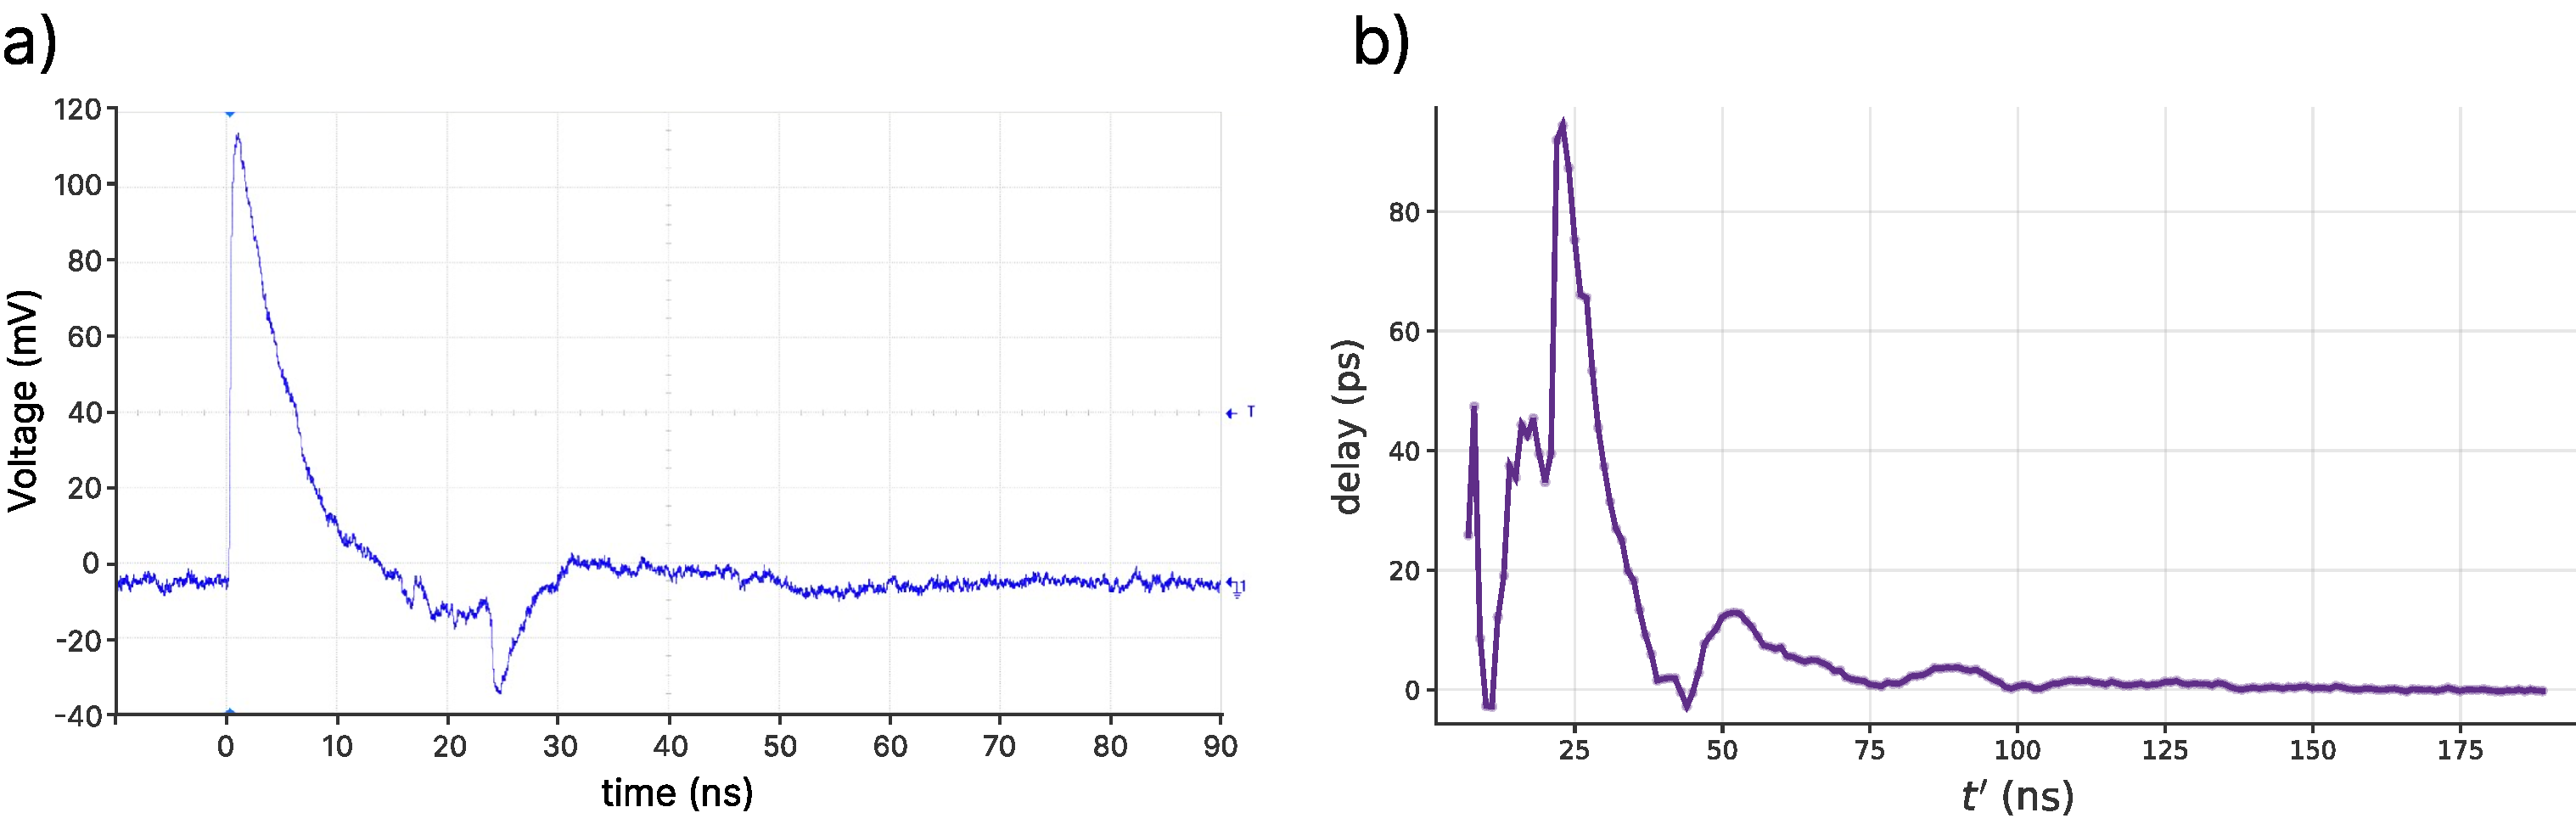
\includegraphics[width=1\textwidth,height=\textheight]{./chapter_03/figs/SOM_Figure_order_1st_v2_light.pdf}
\caption[{PEACOQ RF pulse and calibration curve}]{\textbf{PEACOQ RF pulse and calibration curve} a) The RF pulse of one of the PEACOQ nanowires. The effect of an impedance mismatch reflection is visible at 25~ns. b) The delay vs $t'$ curve for wire 1 of the PEACOQ. The peak at 25~ns lines up in time with the RF reflection visible in (a), and works to correct for the time-walk delays it causes.}
\label{fig:order_1st}
\end{figure}
}

As before with the meandered SNSPD, there is no requirement that the calibration only be used in an application that's based on the same repetition rate of 1 Ghz. As interpolation between points on the delay vs.~$t'$ vslookup curve is possible, delay corrections for arbitrary $t'$ measurements may be found.

\hypertarget{second-order-calibration}{%
\subsubsection{Second Order Calibration}\label{second-order-calibration}}

The 2nd order time-walk correction is a new technique that builds on the methods previously introduced in this chapter. The intrinsic reset time of the PEACOQ nanowires is considerably shorter than the time it takes an RF pulse to return to a steady zero voltage. So multiple pulses can arrive in the time it takes one RF pulse to fully decay as seen by the timing electronics. Therefore, a given RF pulse can be level shifted not only by the presence of a previous pulse a few nanoseconds earlier, but even by the presence of two previous pulses. The calibration and correction process was extended to correct a given pulse timing measurement based on two inter-pulse time measurements $t'$ and $t''$ as shown in Fig.~\ref{fig:order_2nd} a. The calibration process uses the same mode-locked laser derived pulse train as the 1st order calibration. For each $t'$ there is a full range of possible $t''$ times and vice versa, so the result of calibration becomes a 2D grid of delay corrections indexed by $t'$ and $t''$. $t'$ is always less than $t''$ for the parameterization chosen, where both are measured from the latest or `current' time tag (Fig.~\ref{fig:order_2nd} a). Therefore, the space of valid measurements is triangular as shown in Fig.~\ref{fig:order_2nd} b.

\hypertarget{fig:order_2nd}{%
\begin{figure}
\centering
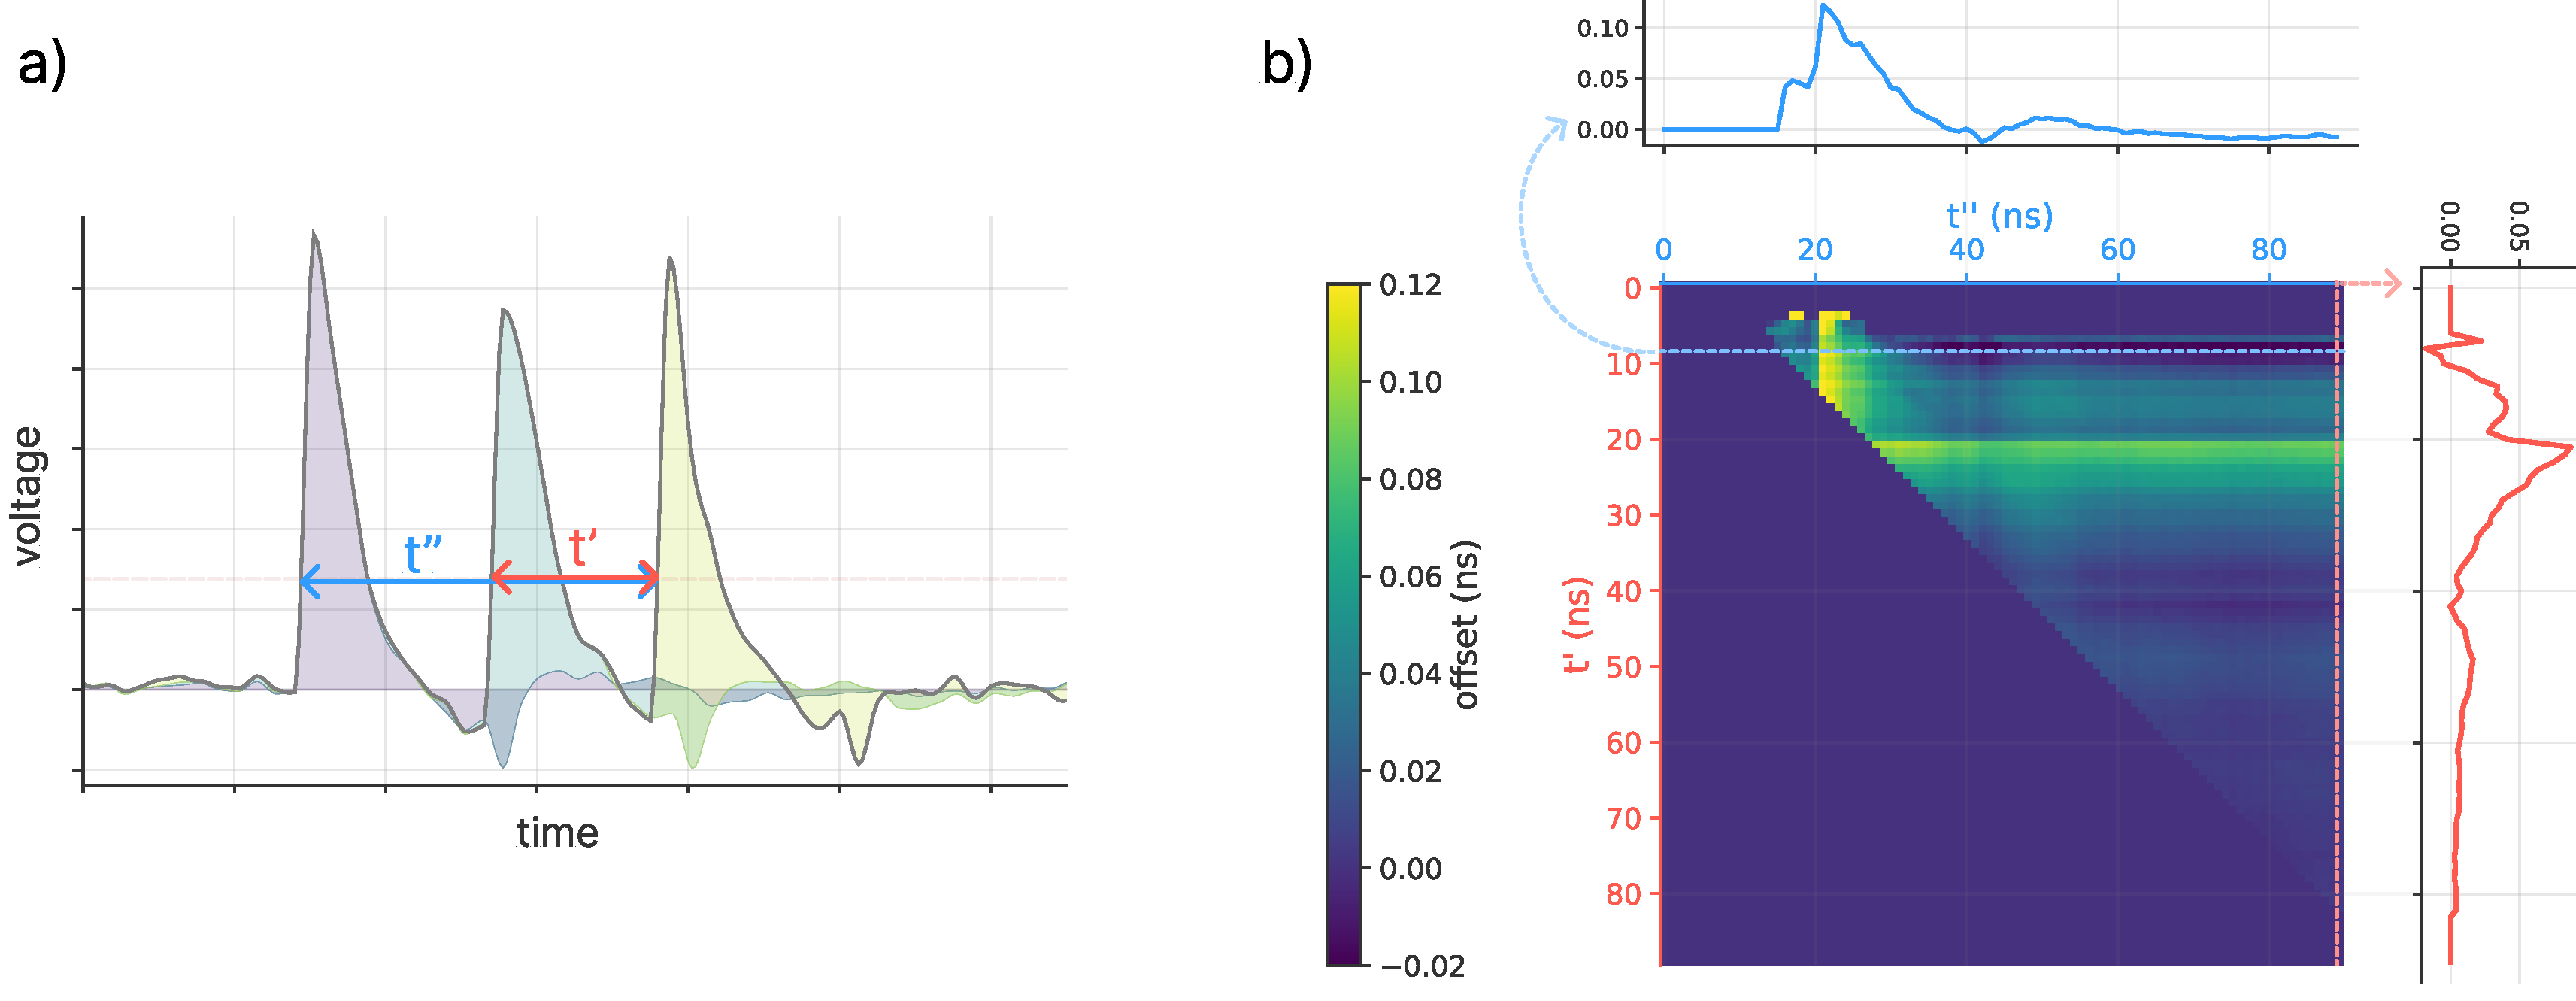
\includegraphics[width=1\textwidth,height=\textheight]{./chapter_03/figs/SOM_Figure_order_2nd_v1_light.pdf}
\caption[{PEACOQ 2D calibration parameterization \& results}]{\textbf{PEACOQ 2D calibration parameterization \& results} a) A diagram showing how RF pulse waveforms can interfere additively, and how $t'$ and $t''$ are parameterized. For illustrative purposes only. b) The result of 2nd order calibration, a grid of delay measurements indexed by $t'$ and $t''$. The blue/red slices and corresponding graphs show how the the effect of varying $t''$ for a given $t'$ is similar to varying $t'$ for a given $t''$.}
\label{fig:order_2nd}
\end{figure}
}

Predominant features of the 2d calibration grid seem to be orthogonal and aligned to the axes. This is a result of the parametrization chosen for $t'$ and $t''$. Features of the calibration that arise due to additive mixing of overlapped RF pulse waveforms which manifest as orthogonal structures in the 2d-calibration grid.

In the limit of large $t''$, a slice of the calibration grid bears close resemblance to the $t'$ vs delay curve used for 1D calibration and correction (Fig.~\ref{fig:order_1st} b). Like in the 1D correction method, a delay correction can be found during real-time acquisition and processing by interpolating on a lookup table. Only now, the lookup table has an extra dependent variable $t''$, and the interpolation is two dimensional.

Proper handling of inter-pulse arrival measurements that fall outside the 2D grid is necessary for good correction performance. When both $t'$ and $t''$ fall outside the 2D grid, no correction is applied. When $t''$ falls outside the grid but $t'$ does not, a 1st order correction is applied to determine what delay must be subtracted to the current tag to correct its distortion. When both $t''$ and $t'$ fall within the 2d grid, a full 2d spline interpolation on the grid in Fig.~\ref{fig:order_2nd} b is applied to find the necessary delay correction.

Like the 1st-order correction, the 2nd-order method makes the assumption that the delays to be corrected are small relative to the inter-pulse times $t’$ and $t’’$.

The codebase supporting our findings with the 1st and 2nd order correction is
available at \href{https://github.com/sansseriff/SNSPD-time-walk-and-jitter-correction}{SNSPD-time-walk-and-jitter-correction}.

{}

\hypertarget{performance-regime-of-the-tungsten-silicide-detector}{%
\subsection{Performance Regime of the Tungsten Silicide detector}\label{performance-regime-of-the-tungsten-silicide-detector}}

When our calibration and correction method is applied to the Tungsten Silicide SNSPD, the walk-cancellation method primarily corrects for pulse height variations. These variations are caused by varying levels of bias current in the device at the time of photo-detection. An oscilloscope trace shows an exponentially decaying increase in SNSPD pulse height following a previous detection. This exponential recovery shape reinforces evidence that this detector operates in this `bias current recovery' regime, rather than the regime where amplifier reset dynamics dominate.

\hypertarget{fig:rise_exp}{%
\begin{figure}
\centering
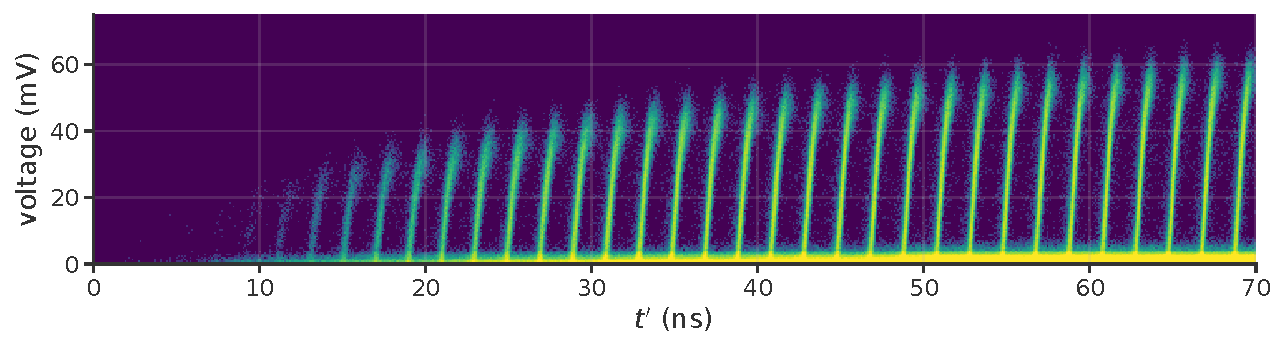
\includegraphics[width=1\textwidth,height=\textheight]{./chapter_03/figs/rise_exp_light.pdf}
\caption[{WSi pulse exponential pulse recovery}]{\textbf{WSi detector pulse recovery} Sweep of trigger levels for pulse rising edges after a previous pulse (not shown). This is similar to a scope trace in overlay false color mode. The detector is illuminated by a 537.5 MHz pulse train.}
\label{fig:rise_exp}
\end{figure}
}

\hypertarget{software-dead-time-for-high-count-rate-jitter-suppression}{%
\subsection{Software dead time for high count rate jitter suppression}\label{software-dead-time-for-high-count-rate-jitter-suppression}}

In certain cases a software-based dead time is an effective way of reducing jitter at high count rates. SNSPD pulses that arrive soon after a previous pulse are ignored because their timing is assumed to be corrupted due to pulse distortions (Fig. \ref{fig:dead_time}a). With a long software-based dead time, data is filtered to keep only events for which the SNSPD was in a fully reset state prior to detection. This results in low jitter measurements even at high rate as shown in Fig. \ref{fig:dead_time}d where the dashed and solid (red, orange) lines are response functions of unfiltered and filtered data respectively. However, the use of software-based dead times can severely limit usable count rate. This paradoxically contrasts with the main intended goal, which is to operate an SNSPD at the highest possible count rates. As shown in the Fig. 3b, adding a 100 ns software dead time to our WSi single pixel SNSPD limits its usable maximum count rate to about 4 MHz, while the raw count rate exceeds 10 MHz. Furthermore, the usable count rate drops to zero for higher incident photon rates, as the dead time starts to reject most events. This behavior can be unexpected and problematic for any applications that occasionally over-saturate the detector.

\hypertarget{fig:dead_time}{%
\begin{figure}
\centering
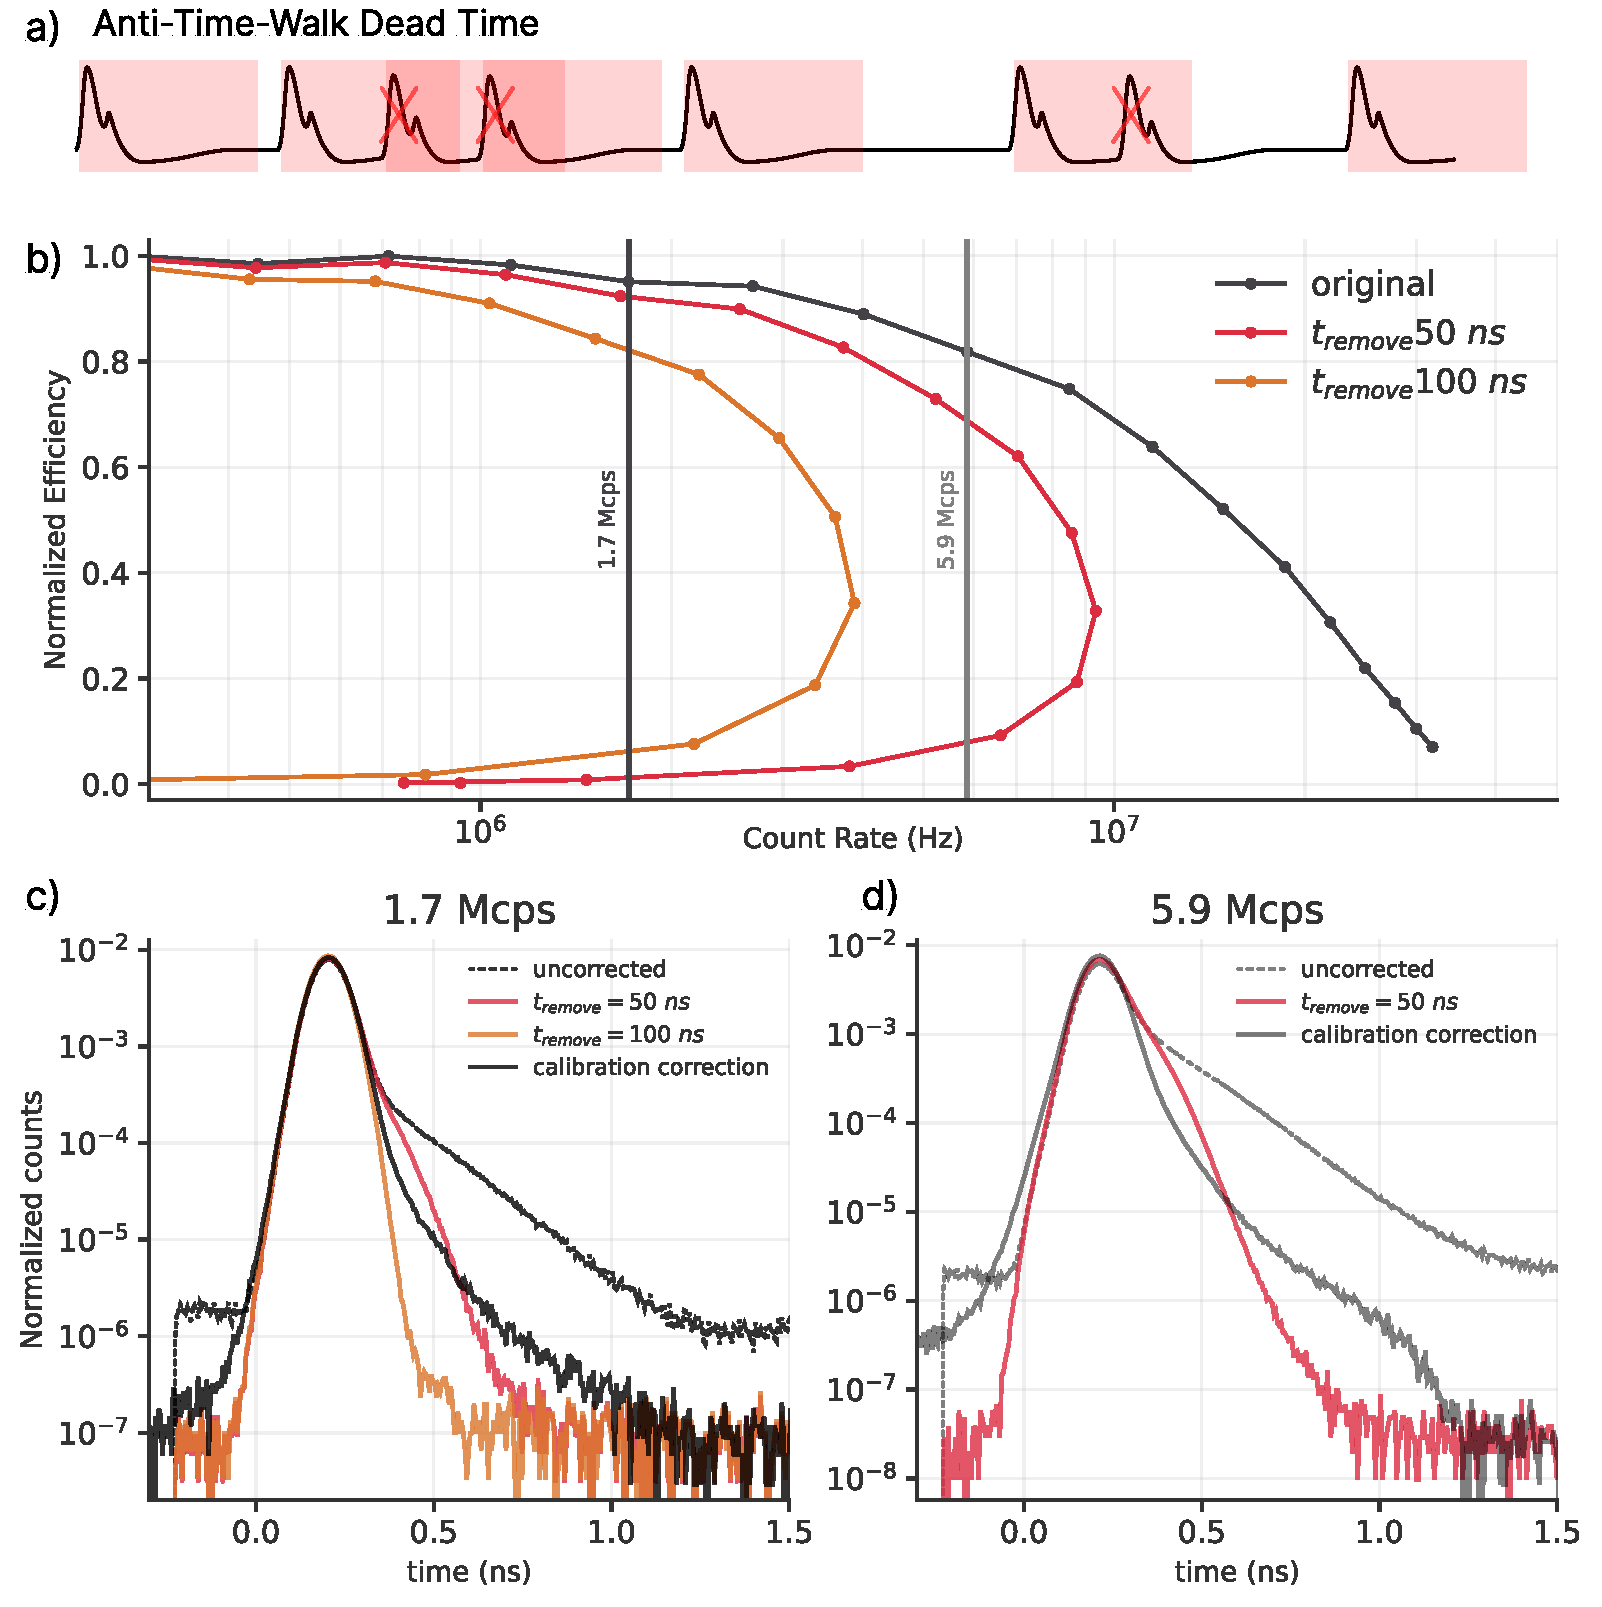
\includegraphics[width=0.8\textwidth,height=\textheight]{./chapter_03/figs/cut_count_rate_v2_light.pdf}
\caption[{Removing time walk with dead time}]{\textbf{Removing time walk with dead time} a) Illustration of the RF signal out of an SNSPD with red highlighted regions signifying a software-based dead time that rejects some events. b) Count rate vs normalized efficiency, similar to the curve in green in Fig.~\ref{fig:jitterate_results_2}. (c) \& (d) Response functions for timetaggs at two count rates denoted by the vertical lines in (b), similar to Fig.~\ref{fig:jitterate_results_2} (b) and (c). The dark grey solid lines show response functions from the calibration and correction method which does not limit count rate. The 100 ns dead time filtered data does not reach the 5.9 Mcps of figure (d) and is therefore not shown in (d).}
\label{fig:dead_time}
\end{figure}
}

\hypertarget{conclusion-outlook}{%
\section{Conclusion \& Outlook}\label{conclusion-outlook}}

The original research paper on time walk analysis \autocite{Mueller2023} included comments on the potential for time walk correction in situations where the reset reset time of the nanowire is considerably shorter than the reset dynamics of the amplifier chain:

\begin{quote}
To optimally correct for this, higher-order correction techniques are needed based on higher-dimensional lookup tables. There is an avenue for exploring such methods for unique use-cases. \autocite{Mueller2023}
\end{quote}

This potential for higher order correction methods turned out to be fruitful, which is why the prior section about \href{section_05_peacoq_2nd_order.md\#second-order-calibration}{higher corder correction} adapted from the PEACOQ paper \autocite{Craiciu23} is included. The original paper went on to claim that there are avenues for exploring time walk correction for pulses measured at multiple voltage levels, or even fully digitized pulses captured with high speed ADCs and FPGAs. These more rigorous readout techniques may be needed to deconvolve photon timing and Photon Number Resolution (PNR) effects from the same nanowire at high count rates~\autocite{Hao2021}. While drafting this thesis, methods for simultaneous time walk correction and PNR correction have not been demonstrated in the literature. However, I believe there is imminent potential to extend the gaussian mixture model methods introduced in the next section for these purposes.

There are other types of extensions and modifications to the presented time walk correction method that may prove to be useful. However, the single-$\Delta t$ measurement approach primarily detailed in this chapter is broadly applicable and straightforward to implement. For insight into developing a streamlined calibration process and in-situ time walk correction as part of larger quantum communication experiments, see the section \ref{time-walk-correction}.

As applications like LIDAR and quantum communication demand ever higher data rates, multiple techniques for increasing photon and data throughput of SNSPD systems are being explored. Arrays or multi-channel SNSPD systems will play a role in satisfying that demand. However, compared to multiple lower count rate SNSPDs operating in parallel, a single detector operating at high rate has certain advantages. First, it makes more efficient use of the extensive bandwidth of the RF readout channel. Second, the single detector with single readout line puts less thermal load on the cooling system than multiple detectors with multiple readout lines. Therefore, paths toward operating individual SNSPDs at the limits of their count rate performance should be explored before extending to multi-pixel systems. This work is a step towards unlocking all available performance and timing precision of SNSPDs operated at high count rates.

\hypertarget{data-recovery-and-pulse-position-modulation-with-a-photon-number-resolving-snspd}{%
\chapter{Data Recovery and Pulse Position Modulation with a Photon Number Resolving SNSPD}\label{data-recovery-and-pulse-position-modulation-with-a-photon-number-resolving-snspd}}

A version of this chapter will be submitted the the journal optics express. A preprint is released as \textbf{\hl{arxiv citation here}}

\hypertarget{abstract-2}{%
\section{Abstract}\label{abstract-2}}

Superconducting Nanowire Single Photon Detectors are a type of time-correlated photon detector with low jitter performance especially in the mid-infrared. They are useful for classical communication over high loss channels --such as across deep space-- and for quantum communication for which signals are restricted to the few-photon level. For classical communication, high photon information efficiency communication may be achieved with Pulse Position Modulation (PPM) whereby data is encoded in the arrival time of an optical pulse with respect to a clock. In the process of demonstrating PPM on a 20~Ghz clock, we study the effects of Photon Number Resolution (PNR) in new low-jitter types of SNSPDs. These PNR effects complicate fixed-threshold triggering of RF pulses from the SNSPD, and corrupt arrival time measurements if not properly managed. We demonstrate methods for simultaneous arrival time and photon number measurement which enables high clock rate PPM for space applications as well as high rate quantum communication and computing applications that benefit from photon number resolution.

\hypertarget{introduction-3}{%
\section{Introduction}\label{introduction-3}}

Deep space optical communication has been a growing field of study in recent years, as space agencies look for ways to increase data rates to and from deep space missions. A key challenge in the development of this technology is closing the communication link over extremely large distances and high loss. This must be done given a restricted power budget available on the spacecraft, and therefore requires the use of photon efficient communication protocols that optimize the number of bits sent per unit of energy.

In this article, we demonstrate high rate Pulse Position Modulation (PPM) applicable to future deep space communication. This starts with a transmitter that sends an optical pulse in one of $2^M$ possible time slots measured with respect to a clock. At a receiver, the arrival time of this pulse is measured to recover $M$ bits of encoded data. Each successive set of $2^M$ time slots following by a dead time constitute a PPM frame.

The Deep Space Optical Communicaiton (DSOC) project managed by the Jet Propulsion Laboratory (JPL) aims to demonstrate optical communication using PPM with the Psyche spacecraft from distances of 0.06 to 2.7 Au \autocite{Srinivasan2023GroundReceiver}.

For larger M, more data may be sent with a single optical pulse, thereby allowing a power limited spacecraft to send more data over a high loss optical channel back to earth. This is quantified through the photon information efficiency $c_p = C/E$ where $C$ is the link capacity and $E$ is the photon cost per optical pulse

The DSOC project uses M at least as high as 5, meaning 5 bits of data are send using 32 time slots per frame. M values as high as 19 have been demonstrated in the lab~\autocite{essiambre2023record}, but the number of time bins needed per frame scales exponentially with the number of bits transmitted per pulse. Therefore, for a given fixed clock rate and time bin duration, the PPM data rate decreases dramatically for higher M values.

We demonstrate a high clock rate PPM protocol in the lab based on modulating a mode-locked laser and receiving pulses with a low jitter superconducting nanowire single photon detector (SNSPD) (Fig.~\ref{fig:intro} (a)).We focus on demonstrating moderately large PIE, while also increasing the clock rate of the sytem by an order of magnitude relative to the DSOC platform (2~GHz). By operating at both higher clock rate and PIE than DSOC, this system exemplifies how future iterations of DSOC may send data more quickly but also over greater distances with the same power budget.

The rate increase is possible due to recent advancements in Niobium Nitride SNSPDs~\autocite{Colangelo2023}. These achieve low jitter performance by incorporating impedance matching tapers for efficient RF coupling, resulting in higher slew rate pulses, and by enabling RF pulse readout from both ends of the nanowire. The dual-ended readout allows for the cancellation of jitter caused by the variable location of photon arrival along the meander when the differential signals are recombined with a balun. These detectors achieve jitter as low as 50 ps at the FW(1/100)M level, making them suitable for the demonstration of PPM with 50 ps slot widths and a 20 GHz clock.

\hypertarget{fig:intro}{%
\begin{figure}
\centering
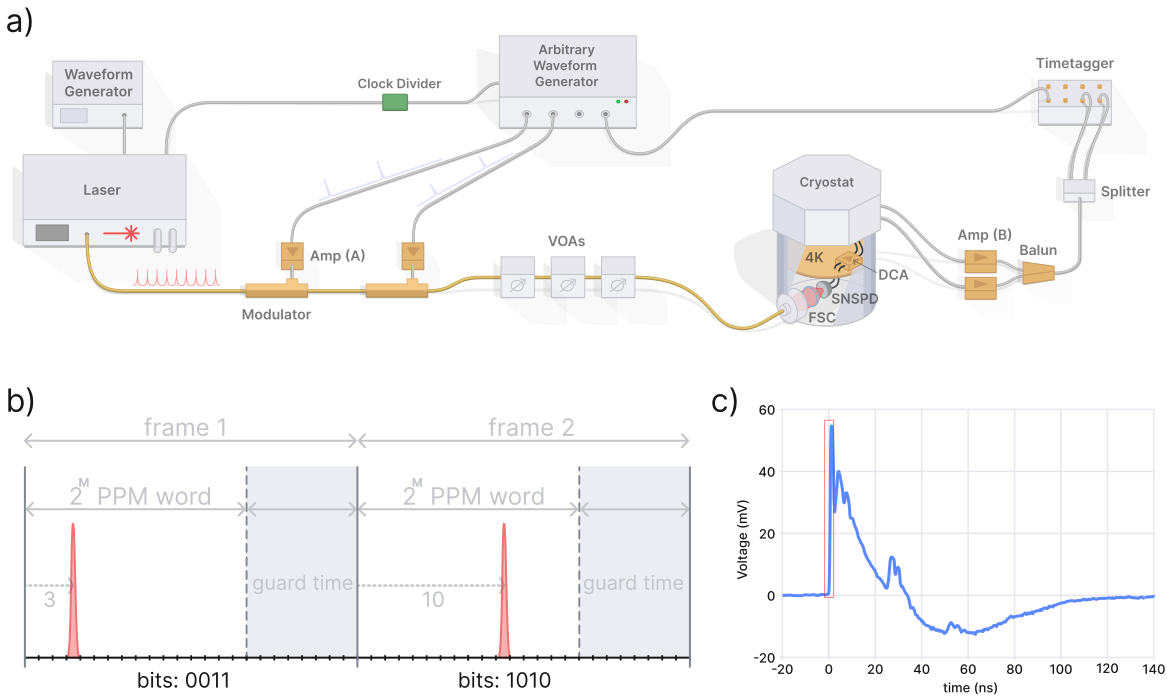
\includegraphics[width=1\textwidth,height=\textheight]{./chapter_04/figs/fig_intro_2_light.pdf}
\caption[{PPM modulation and experiment setup}]{\textbf{PPM modulation and experiment setup} a) Diagram of the expiremental setup. WG: wave generator, CD: clock divider board, AWG: Arbitrary Waveform Generator, MLL: Mode Locked Laser (Pritel UAC), IM: Intensity Modulator, BC: Bias Controller, FSC: Free Space Coupling System, DCA: DC Coupled Cryo-amp b) How bits are transmitted in M=16 PPM modulation. An optical pulse is transmitted with a clock-referenced integer delay which encodes 4 bits of data. c) Scope trace of the RF pulse produced by the differential-readout tapered SNSPD. Fig.~\ref{fig:waveform} zooms in on the rising edge outlined in red here}
\label{fig:intro}
\end{figure}
}

However, these detectors exhibit photon number number dependent responses that affect the time-correlated measurements needed for high-rate PPM. This behavior, shown in Fig.~\ref{fig:waveform} is also known as photon number resolution (PNR) -- a property that is desirable in certain applications including quantum communication and quantum computing. The SNSPD generates RF pulses with greater amplitude and slew rate when detecting optical pulses with multiple photons. Photon number effects are especially evident in this lower jitter variety of SNSPD due to the use of impedance matching tapers which more efficiently couple energy out of the nanowire and into the readout circuit. With high resolution time tagging equipment, photon number dependent effects have even been observed in SNSPDs not necessarily designed to exhibit it \autocite{schapeler2023superconducting,sauer2023resolving} like those without tapers \autocite{Cahall2017SlewRatePNR}. Therefore it is increasingly likely that future research involving low-jitter SNSPDs and multiphoton pulsed sources will have to explicitly manage the PNR response for accurate time-correlated measurements -- whether the effect it is desired or not.

For the tapered differential detectors, the PNR response affects timing of fixed threshold timetaggs at any trigger level (Fig.~\ref{fig:waveform}). However, at higher trigger levels the PNR response is less pronounced and the timing measurements are less affected. Therefore, we divide a single SNSPD readout line using an RF splitter and trigger on the RF pulse at a high and low level as shwon by the red lines in Fig.~\ref{fig:waveform}. This allows us to extract the somewhat conjugate information of pulse arrival time and photon number. From these measurements we study the PNR response in detail and present two methods for managing it. We demonstrate how the photon number information may be deconvolved from the arrival time information, and how both de-correlated degrees of freedom can be extracted simultaneously. This enables the original goal of high rate PPM, but also informs how low-jitter photon number resolving SNSPDs can be used in other classical communication and quantum applications.

\hypertarget{fig:waveform}{%
\begin{figure}
\centering
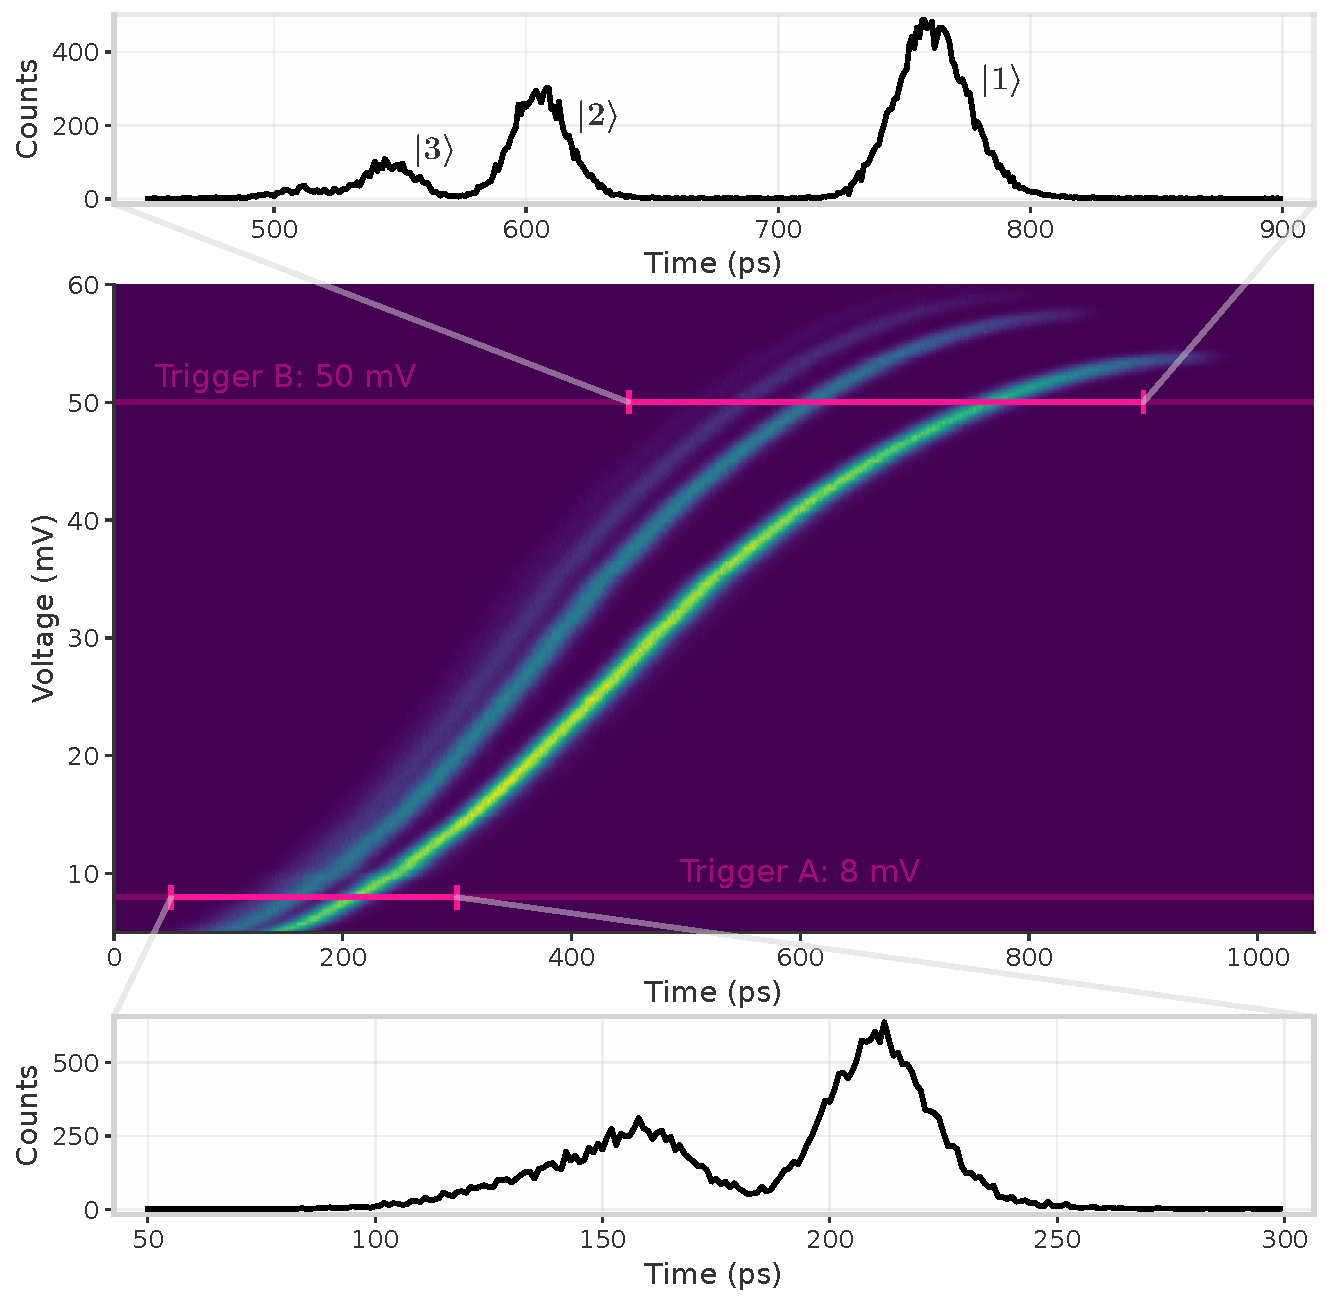
\includegraphics[width=0.8\textwidth,height=\textheight]{./chapter_04/figs/waveform_light.pdf}
\caption[{PNR-sensitive Pulse Waveform}]{\textbf{PNR-sensitive Pulse Waveform} The rising edge of the differential SNSPD's RF pulses exhibit variations in height, slew rate, and arrival time due to photon-number dependent dynamics. The slopes of the 1-photon and 2-photon pulses significantly differ, and as the photon number increases, the alterations to the pulse shape become progressively smaller. Trigger levels A (8~mV) and B (50~mV) were used to extract as much information about pulse slope and arrival time as possible}
\label{fig:waveform}
\end{figure}
}

\hypertarget{detector-figure-of-merit}{%
\section{Detector Figure of Merit}\label{detector-figure-of-merit}}

The work here highlights the application of low jitter single-photon detectors for optical communication, which is impactful for deep-space optical communication as well as classical communication in quantum networks. Although single-photon counting is well estanblished for deep-space optical communication~\autocite{Srinivasan2023GroundReceiver} so far it has not been ulitized in quantum networks, mainly due to the use of SFP modules and DWDMs. However, with the eachievement of high data rates recently achieved with photon-counting classical communication, these approaches can now be seriously considered for quantum networks. The main driver is the reduction of optical power in neighbouring DWDM channels, which ultimately lowers the Raman scattered photons into the quantum channel \autocite{EraerdsRaman}
\textbf{\hl{Calculate reduction in power from state of the art SFP modules}}

To access the applicability of different detectors, here we compare some of the recent near infrared detectors.

A useful figure of merit that includes all of the revelant detector metrics for photon timing was introduced by Bronzi and co-authors \autocite{Bronzi2016}

$$FoM_T = \frac{\eta  (1 - P_{ap})\Phi_{-3 \text{dB}}}{J} \sqrt{\frac{A}{D}},$$

where $\eta$ is the single photon detection efficiency, $\Phi_{-3 \text{dB}}$ is the photon flux at which the system detection efficiency drops by 3~dB, $P_{ap}$ is the afterpulsing probability, $J$ is the detector jitter evaluated as the FWHM, $T_d$ is the deadtime, $A$ is the active area and $D$ is the dark count rate. Here we have defined the maximum photon flux as the 3~dB point, for ease of standardization.

In this work:

\begin{itemize}
\tightlist
\item
  Efficiency = 0.84
\item
  Afterpulsing = 0 \%
\item
  Jitter = 15 ps
\item
  Deadtime = 30 ns \textbf{\hl{measure 3dB flux}}
\item
  Area = 330 $\mu m^2$
\item
  Dark count rate = 20~Hz
\end{itemize}

$FoM_T = 7.58 \times 10^{12}$ at 1550 nm.

The deadtime is calculated as the 1/MCR, which is the 3 dB point of the nominal efficiency. This is only a factor of 3.7 less than the state of the art visible Silicon SPADs (peak efficiency at 480~nm) \autocite{Gramuglia2022}

In the future, the performance of the optical communication system could be improved by using, high count rate SNSPD arrays. Recently published high-count rate arrays have figures of merit of \textbf{\hl{$FoM_T$ for Peacoq and Resta2023 results}}. This would result in a proportinal increase in the data rate.
\textbf{\hl{$FoM_T$ for fastest InGaAs/InP gated detector}}
These devices are ideal for fiber-based optical communication. In free-space, the active area is especially important, whithout the use of an adaptive optics system.
\textbf{\hl{$FoM_T$ for DSOC array}}

\hypertarget{development-of-a-modulation-source}{%
\subsection{Development of a modulation source}\label{development-of-a-modulation-source}}

DSOC relies on modulation of a CW seed laser to generate the communication signal on the spacecraft. This signal is then amplified by an Erbium Doped Fiber Amplifier (EDFA) to increase its transmission power to Earth. As the EDFA amplifies the pre-generated pulses and uses most of the power of the spacecraft optical transmission system, power consumption scales with the number of optical pulses.

We produce our PPM signal signal by carving a high rate mode locked laser with lithium niobate modulators. This way, the jitter of the optical pulses themselves are not limited by the modulators or slew slew rate of the RF signal that drives them. We do two PPM demonstrations, with the source mode locked laser operating at 10.75 and 20 GHz. THe 10.75 GHz demonstration uses a M value of 10, thereby making frames with 1024 time slots of 93 ps width each. The 20 GHz demonstration uses M=11, giving 2048 time slots of 50 ps width per frame. Each frame ends with a dead time of approximately 150 ns to allow the SNSPD to fully recover before the next frame.

Several modern free running time taggers support the averaging of multiple input channels to create fewer higher resolution channels. This implies a tradeoff between jitter or timing resolution and number of channels for a given time tagging device. Therefore, it is important to consider readout methods like that presented here that make use of 2 lower-resolution channels in place of a single higher resolution channel, as these two configurations are similarly resource efficient.

\hypertarget{methods}{%
\section{Methods}\label{methods}}

Prior to the PPM demosntration, we collected data with multi-photon optical pulses repeatedly impinging on the detector at the same time with respect to a clock. This way, we study how the PNR effect in isolation is manifest in the timing measurements recorded at the low and high trigger levels. We label the measurements from the low (8~mV) and high (50~mV) trigger levels as $t_A$ and $t_B$ respectively. As shown in Fig.~\ref{fig:waveform}, histograms of these arrival events are multimodal due to the PNR response. We first present a method for recovering a symmetric arrival time response function using the the slope measurement $\Delta t_{BA} = t_B - t_A$.

\hypertarget{slope-based-correction}{%
\subsection{Slope-Based Correction}\label{slope-based-correction}}

\hypertarget{fig:slope_correction}{%
\begin{figure}
\centering
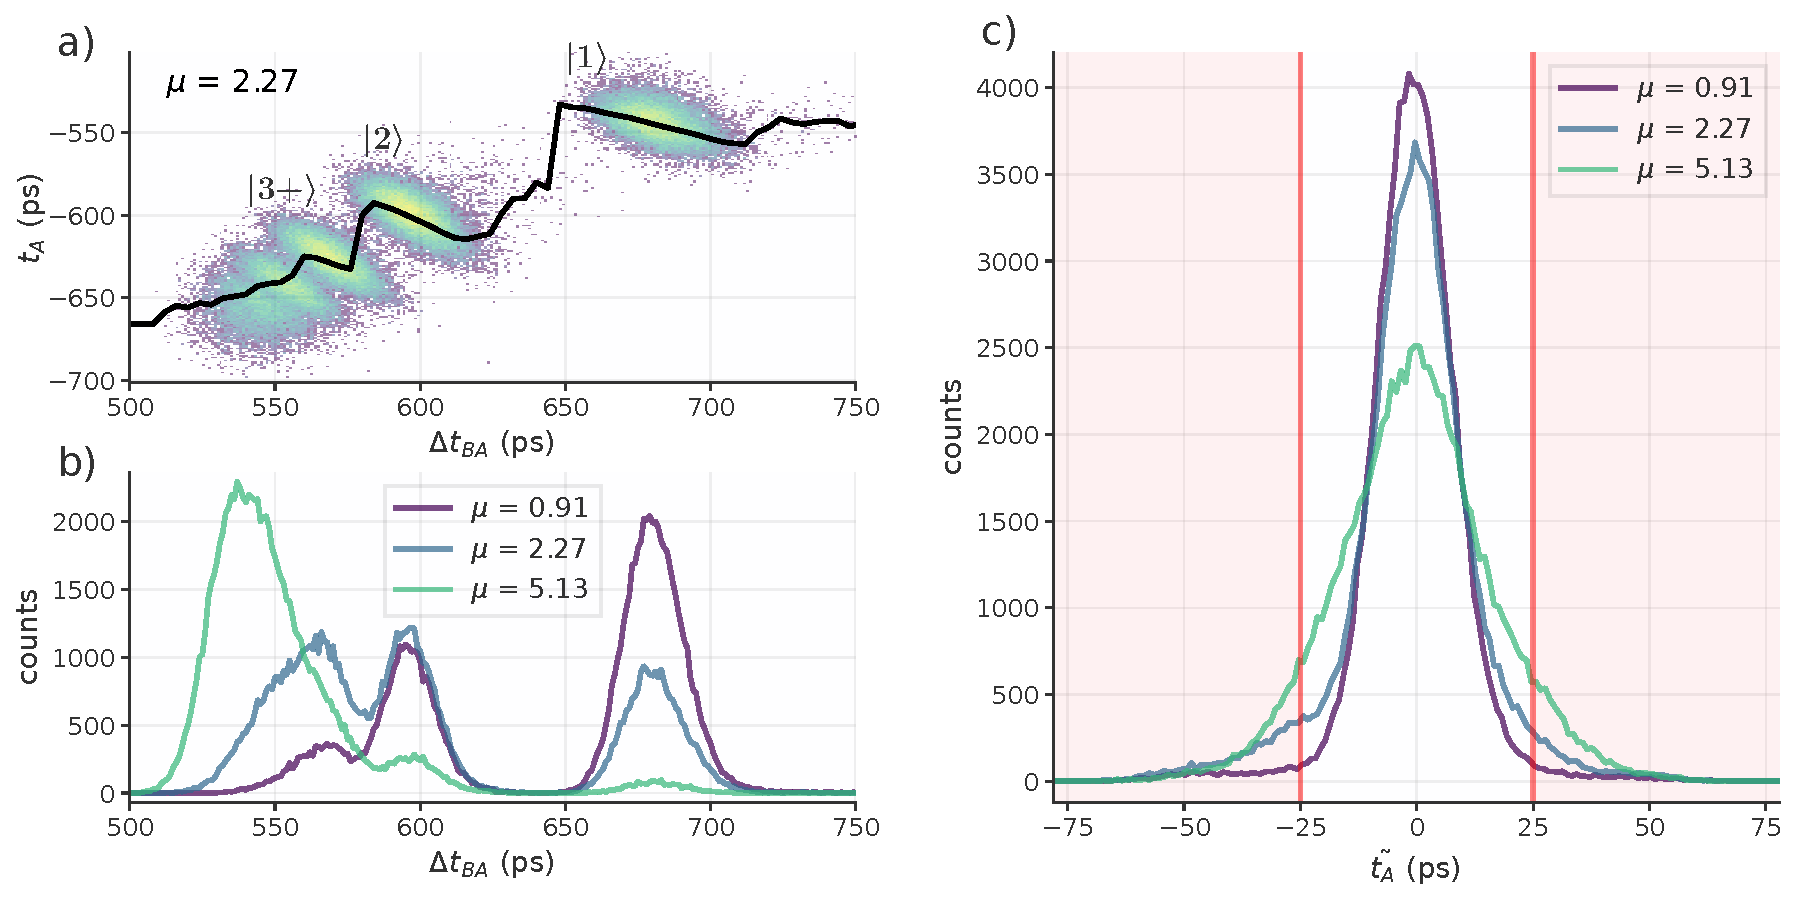
\includegraphics[width=1\textwidth,height=\textheight]{./chapter_04/figs/slope_cancellation_light.pdf}
\caption[{PNR Slope Variation Analysis and Cancellation}]{\textbf{PNR Slope Variation Analysis and Cancellation} a) 2D histogram of RF pulse measurements. Through graphing slope $\Delta t_{BA}$ on the x-axis and arrival time $t_A$ on the y-axis, a series of groupings are visible that identify the discrete photon numbers detected.}
\label{fig:slope_correction}
\end{figure}
}

Pairs of pulse measurements $t_A$ and $t_B$ may be graphed on a 2D plane parametrized by $\Delta t_{BA}$ on the x-axis and $t_A$. Fig.~\ref{fig:slope_correction} a shows how this protection exhibits multiple groupings that correspond the the photon number character of the impinging optical mode. The 1 and 2-photon events are clearly identifiable and seperated from other events, with $|3\rangle$, $|4\rangle$, and $|5\rangle$ events also visible with less mutual separation. While Fig.~\ref{fig:slope_correction} a is shown here for just one mean photon number $\mu$, these grouplings are collected for a full range of attenuations and corresponding $\mu$. Fig.~\ref{fig:slope_correction} a shows histograms from projecting 3 such groupings down onto the $\Delta t_{BA}$ axis.

Thee slope correction method involves the measurement and creation of a slope-versus-arrival time line, one of which is shown in Fig.~\ref{fig:slope_correction} a. This is produced by averaging all $t_A$ measurements for a given slope $\Delta t_{BA}$. That is, the values along vertical slices of the 2D density plot in Fig.~\ref{fig:slope_correction} a are averaged to produce the y-coordinates of the slope-versus-arrival time line shown in black. By interpolating new $\Delta t_{BA}$ measurements on this curve and using it like a lookup table, PNR corrections $C_A$ are found. These may be subtracted off from $t_A$ producting $\tilde{t_A} = t_A - C_A(\Delta t_{BA})$ where $\tilde{t_A}$ is a constructed timing measurement that exhibits a symmetric arrival time response function and shown in Fig.~\ref{fig:slope_correction} c.~

The data representation and calibration curve shown in Fig.~\ref{fig:slope_correction} a may be constructed with $t_B$ on the y-axis as well. Then the PNR corrections are applied the the $t_B$ measurements instead. However, the resulting histograms $\tilde{t_B}$ are virtual identical to $\tilde{t_A}$.

\hypertarget{cluster-analysis}{%
\subsection{Cluster Analysis}\label{cluster-analysis}}

\hypertarget{results}{%
\section{Results}\label{results}}

results here

{}

\hypertarget{discussion}{%
\section{Discussion}\label{discussion}}

We have shown that measurement of the slew rate or slope of SNSPD RF pulses may be useful for both photon number and arrival time discrimination. This is a fairly practical method that limited assumptions about the underlying modulation pattern of the optical signal. We show it allows for the measurement of pulse position modulation signals based on 10 and 20 Ghz clocks for which each optical pulse contains anywhere from 1 to 5 or more photons.

We also present a 2-dimensional gaussian mixture model of the SNSPD response to the two trigger levels in an effort to model the available data as accurately and faithfully as possible. This may be used for photon number and arrival time discrimination as well. Assigning SNSPD detection events to photon number or PPM bins generalizes to assigning points in a 2-dimensional space to probability distributions built from gaussian mixtures. We show the gaussian mixture method moderately improves the accuracy of arrival time discrimination relative to the slope-based method.

The full 2D treatment of photon number discrimination based on community detection of gaussian mixture groups is undeniably more complex than principle component analysis methods demonstrated in previous research\autocite{sauer2023resolving,schapeler2023superconducting}. However, it's generality may be advantageous for future SNSPD systems that gather added data about the transient state of the SNSPD and readout circuitry. For example, more than two timing measurements from each SNSPD pulse may prove to be useful. Recent research has demonstrated that photon number information is present in the falling edge of the pulse \autocite{sauer2023resolving,schapeler2023superconducting}, and, as shown here, timing measurements from two trigger levels on the rising edge are also useful. Therefore, the use of three or more unique time-correlated measurements may be advantageous. Digitizing the RF pulse with a high speed ADC or oscilloscope extends this thinking to many more measurements. Ultimately, photon number discrimination becomes a higher dimensional problem, for which gaussian mixture methods may outperform principle component analysis.

Finally, higher dimensional analysis may be necessary when pulse overlap or time walk effects \autocite{Mueller2023} complicate the nuanced photon number response characteristics of each SNSPD pulse. This is important in future SNSPD systems that are designed to exhibit both high maximum count rates \autocite{Craiciu23} and photon number resolution.

\hypertarget{synchronization-with-a-software-phase-locked-loop-pll}{%
\section{Synchronization with a Software Phase Locked Loop (PLL)}\label{synchronization-with-a-software-phase-locked-loop-pll}}

\textbf{Todo}
\emph{This will be the first place in the thesis that I introduce the use of my software based phase locked loop (PLL). The software PLL has been useful in several later projects. I will either fully explain the PLL here, or I will only introduce and motivate it here. And a full description will go in an appendix. }
1. For sending many PPM symbols, I needed a synchronization clock that was (A) always running, and (B) extremely low jitter.
2. Sending an output from the AWG to the Swabian timetagger in another room resulted in a less-than-ideal clock source. The signal was low amplitude, and triggering on it's rising edge did not make for a very low jitter clock signal.
3. I had some sense that that should be a way of `averaging' past clock cycles in some way to cancel jitter. After some research and failed tests toward developing my own averaging method, I learned a software based Phase Locked Loop is just what I needed.
4. Initial version was adapted from a Matlab code on the Phase Locked Loop wikipedia page. That code was written for a sampled sign wave, but I adapted to take in just one data point per period. For our non-coherent and time-resolved types of measurements with SNSPDs, we typically only have clocks of this type. Where the clock is expressed by some type of optical or RF pulse that arrives on a regular period.
5. More recently Rahaf Youssef and I have worked on updating our software PLL tools so that its easier to understand and reason about, and easier to lock to a given signal.

\hypertarget{high-rate-entanglement-generation}{%
\chapter{High Rate Entanglement Generation}\label{high-rate-entanglement-generation}}

A version of this chapter is currently under review. A preprint is released as:

Andrew Mueller, Samantha Davis, Boris Korzh, Raju Valivarthi, Andrew D. Beyer, Rahaf Youssef, Neil Sinclair, Matthew D. Shaw, \& Maria Spiropulu. (2023). \href{https://arxiv.org/abs/2310.01804}{High-rate multiplexed entanglement source based on time-bin qubits for advanced quantum networks}.

\hypertarget{abstract-3}{%
\section{Abstract}\label{abstract-3}}

Entanglement distribution based on time-bin qubits is an attractive option for emerging quantum networks. We demonstrate a 4.09 GHz repetition rate source of photon pairs entangled across early and late time bins separated by 80 ps. Simultaneous high rates and high visibilities are achieved through frequency multiplexing the spontaneous parametric down conversion output into 8 time-bin entangled channel pairs. We demonstrate entanglement visibilities as high as 99.4\%, total entanglement rates up to 3.55$\times 10^6$ coincidences/s, and predict a straightforward path towards achieving up to an order of magnitude improvement in rates without compromising visibility. Finally, we resolve the density matrices of the entangled states for each multiplexed channel and express distillable entanglement rates in ebit/s, thereby quantifying the tradeoff between visibility and coincidence rates that contributes to useful entanglement distribution. This source is a fundamental building block for high-rate entanglement-based quantum key distribution systems or advanced quantum networks.

\hypertarget{introduction-4}{%
\section{Introduction}\label{introduction-4}}

\hypertarget{fig:system}{%
\begin{figure}
\centering
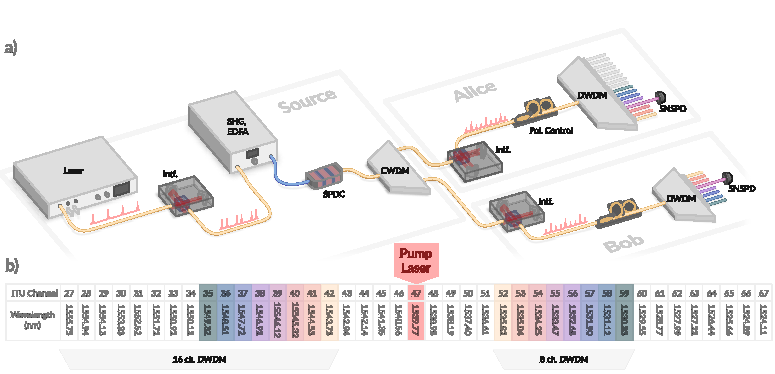
\includegraphics[width=1\textwidth,height=\textheight]{./chapter_05/figs/sys_drawing_light.pdf}
\caption[{Layout of experiment}]{\textbf{Layout of experiment} a) Pulses from a 1539.47 nm mode locked laser (Pritel UOC) are split into two by an 80-ps delay-line interferometer before up-conversion and amplification in a second harmonic generation + erbium doped fiber amplifier (SHG + EDFA) module (Pritel). A short PM fiber from the SHG module connects to a nonlinear crystal generating photon pairs by spontaneous parametric down-conversion (SPDC). The coarse wavelength division multiplexing (CWDM) module separates the photon pair spectrum into eight 13~nm-wide bands around 1530 and 1550 nm, for the signal and idler photon, respectively. The signal and idler are directed to the Bob and Alice stations, respectively. The readout interferometers introduce the same time delay as the source interferometer. Polarization controllers are used to maximize the coincidence rates, as the detection efficiencies of each SNSPD is polarization sensitive ($\pm20\%$). Entanglement visibility is unaffected by readout polarization. 100 GHz spacing Dense wavelength division multiplexer (DWDM) modules are used to direct each frequency channnel into a distinct fiber. Two superconducting nanowire single photon detectors (SNSPDs) are used to measure a specific frequency multiplexed channel pair. Measurements for different multiplexed channels are performed in succession to resolve full system performance. b) ITU channels used in the experiment. Pairs of channels highlighted with the same color obey the phase and pump-energy matching condition for SPDC. To asses the full 16 channels (27-42) of Alice's DWDM multiplexer, Bob's 8-channel DWDM is replaced with a narrowband filter with tunable resonance frequency (not shown in figure).}
\label{fig:system}
\end{figure}
}

Entangled photons play a vital role in the development of quantum information processing and communication systems~\autocite{nielsen2010quantum,ladd2010quantum,gisin2007quantum,pirandola2015advances,briegel1998quantum,kimble2008quantum}. The ability to generate entangled photon pairs at a high rate is essential for establishing reliable and scalable quantum networks with quantum repeaters, as well as for implementing entanglement-based quantum key distribution (QKD) systems~\autocite{Sangouard2011,ma2007quantum,ribordy2000long,yin2017satellite}. Unlike QKD implementations that rely on attenuated lasers~\autocite{sasaki2011field,scarani2009security} entanglement distribution systems may fulfill the objectives of QKD while also serving as the foundation for advanced quantum networks that rely on entanglement as a fundamental resource.

Entanglement distribution and entanglement-based QKD have been demonstrated with impressive performance across a number of metrics. These include 40~kbps data rates in a QKD system deployed over 50~km of fiber~\autocite{Pelet2022} as well as multiple polarization entangled sources that leverage spectral multiplexing. These polarization sources include a demonstration of 181 kebits/s across 150 ITU channel pairs and a high-throughput source potentially capable of gigabit rates with many added channels and detectors \autocite{Alshowkan2022,Neumann2022Entanglement}. Multiple works have highlighted the need to leverage high total brightness, spectral brightness, collection efficiency, and visibility from pair-generating non-linear crystals to realize practical high-rate entanglement distribution~\autocite{Neumann2022Entanglement,atzeni2018integrated,sun2019compact,liu2021device,kaiser2014polarization,anwar2021entangled,neumann2021model}.

A time-bin entangled photon source has certain advantages over a polarization-based system~\autocite{marcikic2002time}. Time-bin entanglement can be measured with no moving hardware and does not require precise polarization tracking to maximize visibility~\autocite{Dong2018PolarizationControll,Fitzke2022TimeBinVsPol}. Also, with suitable equipment, robust time-bin modulation is possible over free space links with turbulence~\autocite{Jin2019}. Therefore, the possibility of simplified fiber-to-free-space interconnects and larger quantum networks based on a shared time-bin protocol motivates development of improved time-bin sources. Furthermore, time-bin encoding is suited for single-polarization light-matter interfaces \autocite[\textcite{lauk2020perspectives}]{simon2010quantum}.

We direct 4.09 GHz mode locked laser light into a nonlinear crystal via 80-ps delay-line interferometers (12.5 GHz free-spectral range) to realize a high-rate entanglement source. The ability to resolve time-bin qubits into 80~ps wide bins is enabled by newly developed low-jitter differential superconducting nanowire single-photon detectors (SNSPDs)~\autocite{Colangelo2023}. Wavelength multiplexing is used to realize multiple high visibility channel pairings which together sum to a high coincidence rate. Each of the pairings can be considered an independent carrier of photonic entanglement~\autocite{Djeylan2016,Wengerowsky2018} and therefore the system as a whole is applicable to flex-grid architectures through the use of wavelength selective switching \autocite{Appas2021,Alshowkan22Switching}. However, we focus on maximizing the rate between two receiving stations, Alice and Bob (Fig. \ref{fig:system}a). Each station is equipped with a DWDM that separates the frequency multiplexed channel into multiple fibers for detection. The SNSPDs are used with a real-time pulse pileup and time-walk correction technique~\autocite{Mueller2023} to keep jitter low even at high count rates.

We quantify per-channel brightness and visibility as a function of pump power, as well as collection efficiencies, coincidence rates across 8 channel pairs, and expected performance of a partially realized 16-channel pair configuration. We show that the 8 channel system achieves visibilities that average to 99.3\% at low mean photon number $\mu_{L} = 5.6{\times} 10^{-5}\,\pm\,9{\times} 10^{-6}$. At a higher power ($\mu_{H} = 5.0{\times} 10^{-3}\,\pm\,3{\times} 10^{-4}$), we demonstrate a total coincidence rate of 3.55 MHz with visibilities that average to 96.6\%. Through quantum state tomography we bound the distillable entanglement rate of the system to between 69\% and 91\% of the $\mu_{H}$ coincidence rate (2.46 - 3.25 Mebits/s).

Quantifying a source's spectral mode purity is important for gauging its utility in advanced quantum networks that rely on interferometric measurements like two-photon interference which enables Bell-state measurements (BSM)~\autocite{Valivarthi2020}.
With Schmidt decomposition we quantify the modal purity of single DWDM channel pairs and derive the inverse Schmidt number which serves as an estimate for two-photon interference visibility between two such sources. Ultimately, we demonstrate that an entanglement generation source of this design makes for a robust and powerful building block for future high-rate quantum networks.

\hypertarget{system}{%
\section{System}\label{system}}

Figure~ Fig.~\ref{fig:system} shows the experimental setup. Pulses from the 4.09 GHz mode-locked laser, with a center wavelength at 1539.47 nm, are sent through an 80 ps delay-line interferometer (Optoplex). This generates the pulses used to encode early/late basis states ($|e\rangle,|l\rangle$), which are subsequently up-converted by a second harmonic generation (SHG) module (Pritel) and down-converted into entangled photon pairs by a type-0 spontaneous parametric down conversion (SPDC) crystal (Covesion)~\autocite{Marcikic2002}. The up-converted pulses at 769 nm have a FWHM bandwidth of 243 GHz (0.48 nm), which along with the phase matching condition of the SPDC waveguide, defines a wide joint spectral intensity (JSI) function~\autocite{kim2005measurement}.

The photon pairs, which are separated by a coarse wavelength division multiplexer (CWDM), are of the form $|\psi\rangle=\frac{1}{\sqrt{2}}\left(|e\rangle_{s}|e\rangle_{i}+e^{i \phi}|l\rangle_{s}|l\rangle_{i}\right)$. Entangled idler and signal photons are sent to the receiving stations labeled Alice and Bob, respectively. One readout interferometer at each station projects all spectral bands into a composite time-phase basis. From here, dense wavelength division multiplexers (DWDM) divide up the energy-time entangled photon pairs into spectral channels.

DWDM outputs are sent to differential niobium nitride (NbN) single pixel SNSPDs~\autocite{Colangelo2023} with 22 × 15~µm active areas formed by meanders of 100-nm-wide and 5-nm-thick niobium nitride (NbN) nanowires on a 500~nm pitch. These measure the arrival time of photons with respect to a clock signal derived from the mode locked laser. Use of the high system repetition rate and compact 80~ps delay interferometers is only possible due to the high timing resolution of these detectors. Low jitter performance is achieved by incorporating impedance matching tapers for efficient RF coupling, resulting in higher slew rate pulses, and by enabling RF pulse readout from both ends of the nanowire. The dual-ended readout allows for the cancellation of jitter caused by the variable location of photon arrival along the meander when the differential signals are recombined with a balun. We use two SNSPDs for this demonstration with efficiencies at 1550~nm of 66\% and 74\%. A full 8-channel implementation of this system would require 16 detectors operating in parallel at both Alice and Bob. To read out both outputs of both interferometers, 4 detectors per channel are required, resulting in 32 detectors total.

A novel time-walk or pulse-pileup correction technique is used to extract accurate measurements of SNSPD pulses that arrive between 23 and 200~ns after a previous detection on the same RF channel. Without special handling of these events, timing jitter will suffer due to RF pulse amplitude variations and pileup effects. As detailed in Supplementary note 3, the correction method works by subtracting off predicable timing distortions based on the inter-arrival time that precedes them~\autocite{Mueller2023,Craiciu23}. An in-situ calibration process is used to build a lookup table that relates corrections and inter-arrival time. At the highest achievable pump power, this correction method leads to 320\% higher coincidence rates compared to a data filtering method that rejects all distorted events arriving within $\simeq$ 200~ns of a previous pulse.

\hypertarget{results-1}{%
\section{Results}\label{results-1}}

By pairing up particular 100~GHz DWDM channels and recording coincidence rates, a discretized form of the JSI of our pair source is measured (Fig.~\ref{fig:figure_2nd_1} a). Due to the wide pump bandwidth, the spectrum of signal photons spans several ITU channels for a given idler photon wavelength. Pairs along the main diagonal are optimized for maximum coincidence rates by tuning the pump laser frequency, and are therefore used for all remaining measurements. In Fig.~\ref{fig:system} b, these pairs are highlighted with matching colors. Coupling efficiencies $\eta$ shown in Fig.~\ref{fig:figure_2nd_1} a are derived from a JSI fitting analysis \textbf{\hl{(see Supplementary note 6)}} and include all losses between the generation of entangled pairs in the SPDC and final photo-detection.

A joint spectral analysis of the 100~GHz fiters applied to the wide-bandwidth pumped JSI shows only a fraction of idler (signal) photons that pass though one filter will be detected with their corresponding signal (idler) photon. This is true even for ideal filters that are 100\% transmissive within their passbands, which demonstrates a geometrical limit on the ratio of coincidence rates to singles rates in this regime of large bandwidth JSI and narrowband filters. For calculations of $\mu$ in terms of coincidence rate $C_{AB}$, repetition rate $R$, and singles rates $S_A, S_B$, we account for this by adding a geometric compensation factor $\delta$ to the commonly used equation:

\begin{align}
\mu =  \frac{\delta S_A S_B}{R C_{AB}}.
\end{align}

This gives a definition of $\mu$ for the JSI region where signal and idler filters overlap according to energy conservation, and the probability of transmitting entangled pairs to both Alice and Bob is non-negligible. It is valid in the low $\mu$ regime where generation of higher order photon number states from the SPDC are rare. For filter pairings along the main diagonal in Fig.~\ref{fig:figure_2nd_1} a, values for $\delta$ are fairly consistent and average to $\delta = 0.393 \pm 0.012$. The derivation of $\delta$ is detailed in \textbf{\hl{Supplementary note 7}}.

\hypertarget{fig:figure_2nd_1}{%
\begin{figure}
\centering
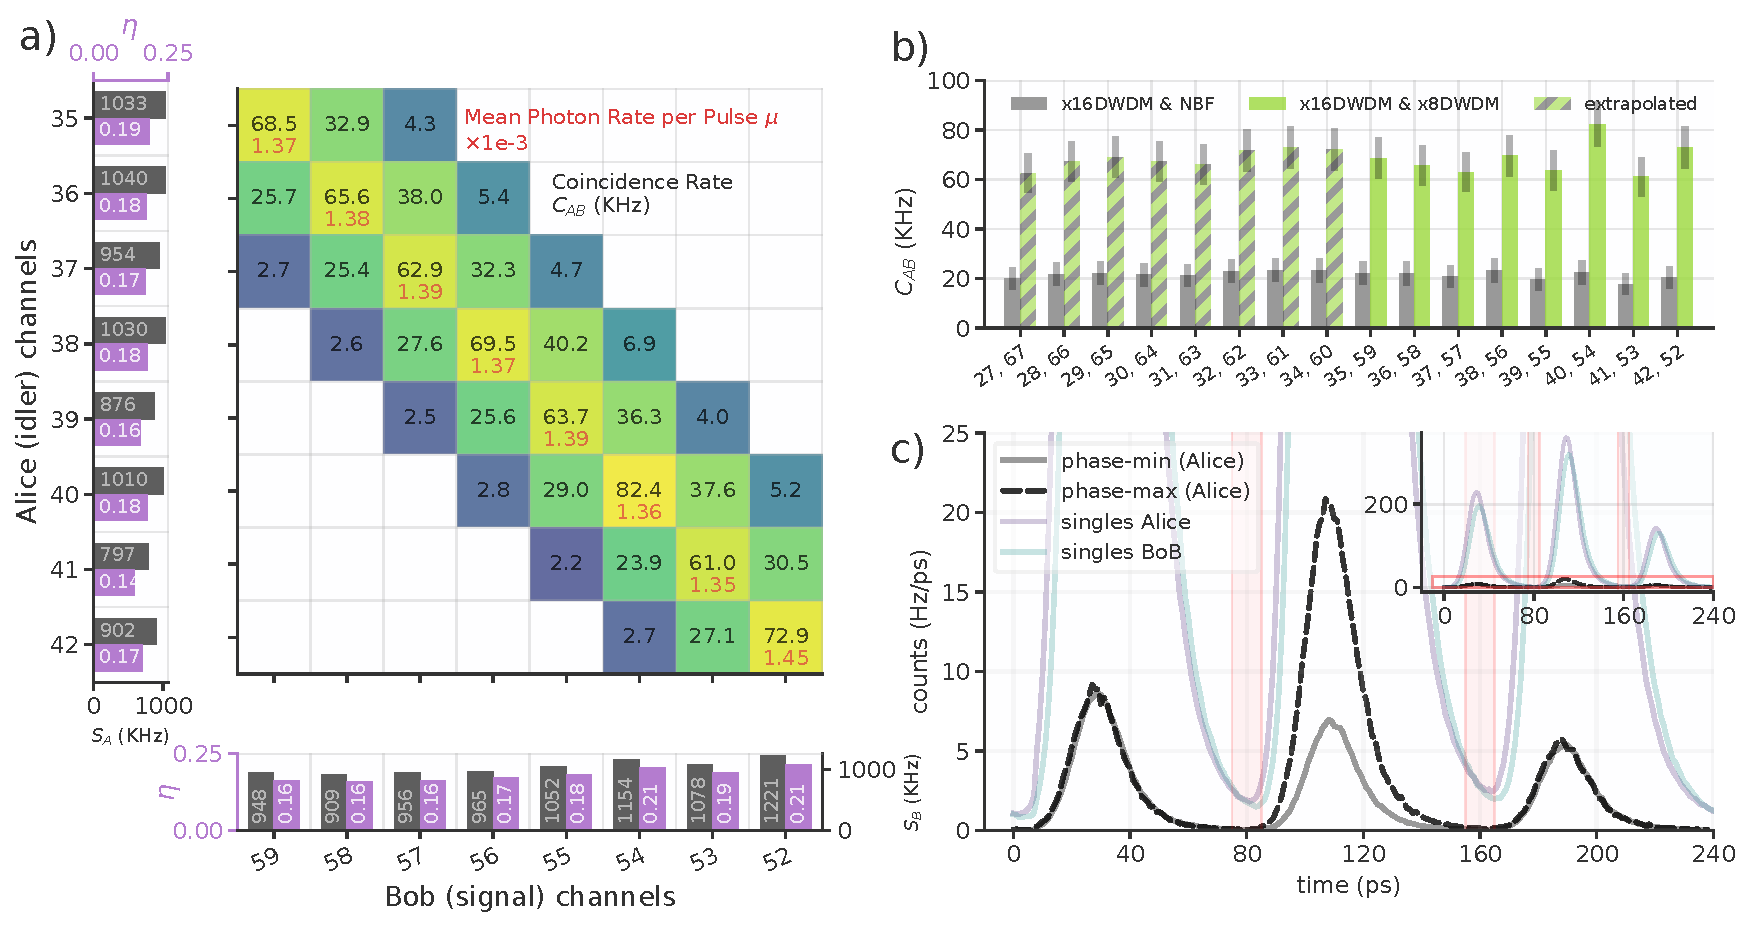
\includegraphics[width=1\textwidth,height=\textheight]{./chapter_05/figs/jsi_figure_light.pdf}
\caption[{Joint spectral intensity measurements and histogram}]{\textbf{Joint spectral intensity measurements and histogram}a) The singles rates at Alice $S_A$ and Bob $S_B$ (grey bars), path coupling efficiencies (purple bars), and coincidence rates $C_{AB}$ (black text in colored boxes) for different DWDM channel pairings. All measurements are recorded at a SHG pump power of 14.6~mW, for which $\mu$ of the channel pairs along the main diagonal are shown in red text. The joint spectral intensity envelop spans several 100 GHz channels. As detailed in Supplement note 2, the coincidence rates (kHz, black) are scaled to represent two branches of the total wavefunction, so that they are consistent with the coupling efficiencies $\eta$ (purple bars) and the singles rates (grey bars). There are four branches for each pairing of the four interferometer output ports. In practice, one output each of Alice and Bob's interferometers is measured, thereby capturing one branch. See Supplement 1 for details of the scaling method, and the fitting method used to solve for the coupling efficiencies $\eta$. b) Coincidence rates for energy-matched channel pairings. The light green bars depict the main diagonal in (a). Grey bars are measured with x16 DWDM at Alice and a tunable narrowband filter at Bob. Dashed bars predict the rates for a system with x16 DWDMs at both Alice and Bob c) Histogram of photon arrival events with respect to the 4.09 GHz clock. Dashed black and grey lines show the response functions for coincidence events. Red bars represent guard regions where coincidence events are ignored. Events within 10~ps guard regions centered at 80 and 160~ps (shaded red) are discarded for analysis of coincidences between individual bins. This is done to maximize visibility in the presence of some minor overlap of the pulses (see \textbf{\hl{Supplementary note 5}} for discussion).}
\label{fig:figure_2nd_1}
\end{figure}
}

In the following, rigorous tests of entanglement are primarily done with the 8 ITU 100 GHz channel pairings: Ch. 35-42 at Alice and Ch. 52-49 at Bob. However, in Fig.~\ref{fig:figure_2nd_1} b we investigate rates across 16 pairs by using all 16 channels available on the DWDM at Alice (24 - 34) and a tunable narrowband filter in place of the DWDM at Bob. As the narrowband filter has higher loss and 45~GHz FWHM passband (see Supplementary note 4 for measurements), the coincidence rates are lower (grey bars in Fig.~\ref{fig:figure_2nd_1} b). But the uniformity of coincidence rates across 16 channels implies that the use of 16-channel DWDMs at both Alice and Bob would roughly double the total coincidence rate.

Signals from the SNSPDs are directed to a free-running time tagger (Swabian) and processed with custom software. The resulting histograms, referenced from a shared clock (Fig.~\ref{fig:figure_2nd_1} c), depict three peaks, which are caused by the sequential delays of the source and readout interferometers. Some intensity imbalance between long and short paths is present in these interferometers, which explains the asymmetry between early and late peaks in Fig.~\ref{fig:figure_2nd_1} c.~Such imbalances are present in both the source and readout interferometers to varying degrees. The interferometer used for the source exhibits an early/late intensity balance ratio of 1.13. Alice and Bob's interferometers exhibit early/late imbalances of 1.24 and 1.15 respectively. An analysis of how this type of imbalance affects entanglement visibility is included in Supplementary note 10.

The coincidence rate across Alice and Bob's middle bins varies sinusoidally with respect to the combined phase relationship of the source and readout interferometers (see Supplementary note 1)~\autocite{Inagaki2013,Marcikic2002}. In Fig.~\ref{fig:figure_2nd_1} c the coincidences shown are for any combination of early, middle, or late bins. For tomography and visibility measurements, coincidence detections across specific bin pairings are considered.\\

\hypertarget{fig:shg_scan}{%
\begin{figure}
\centering
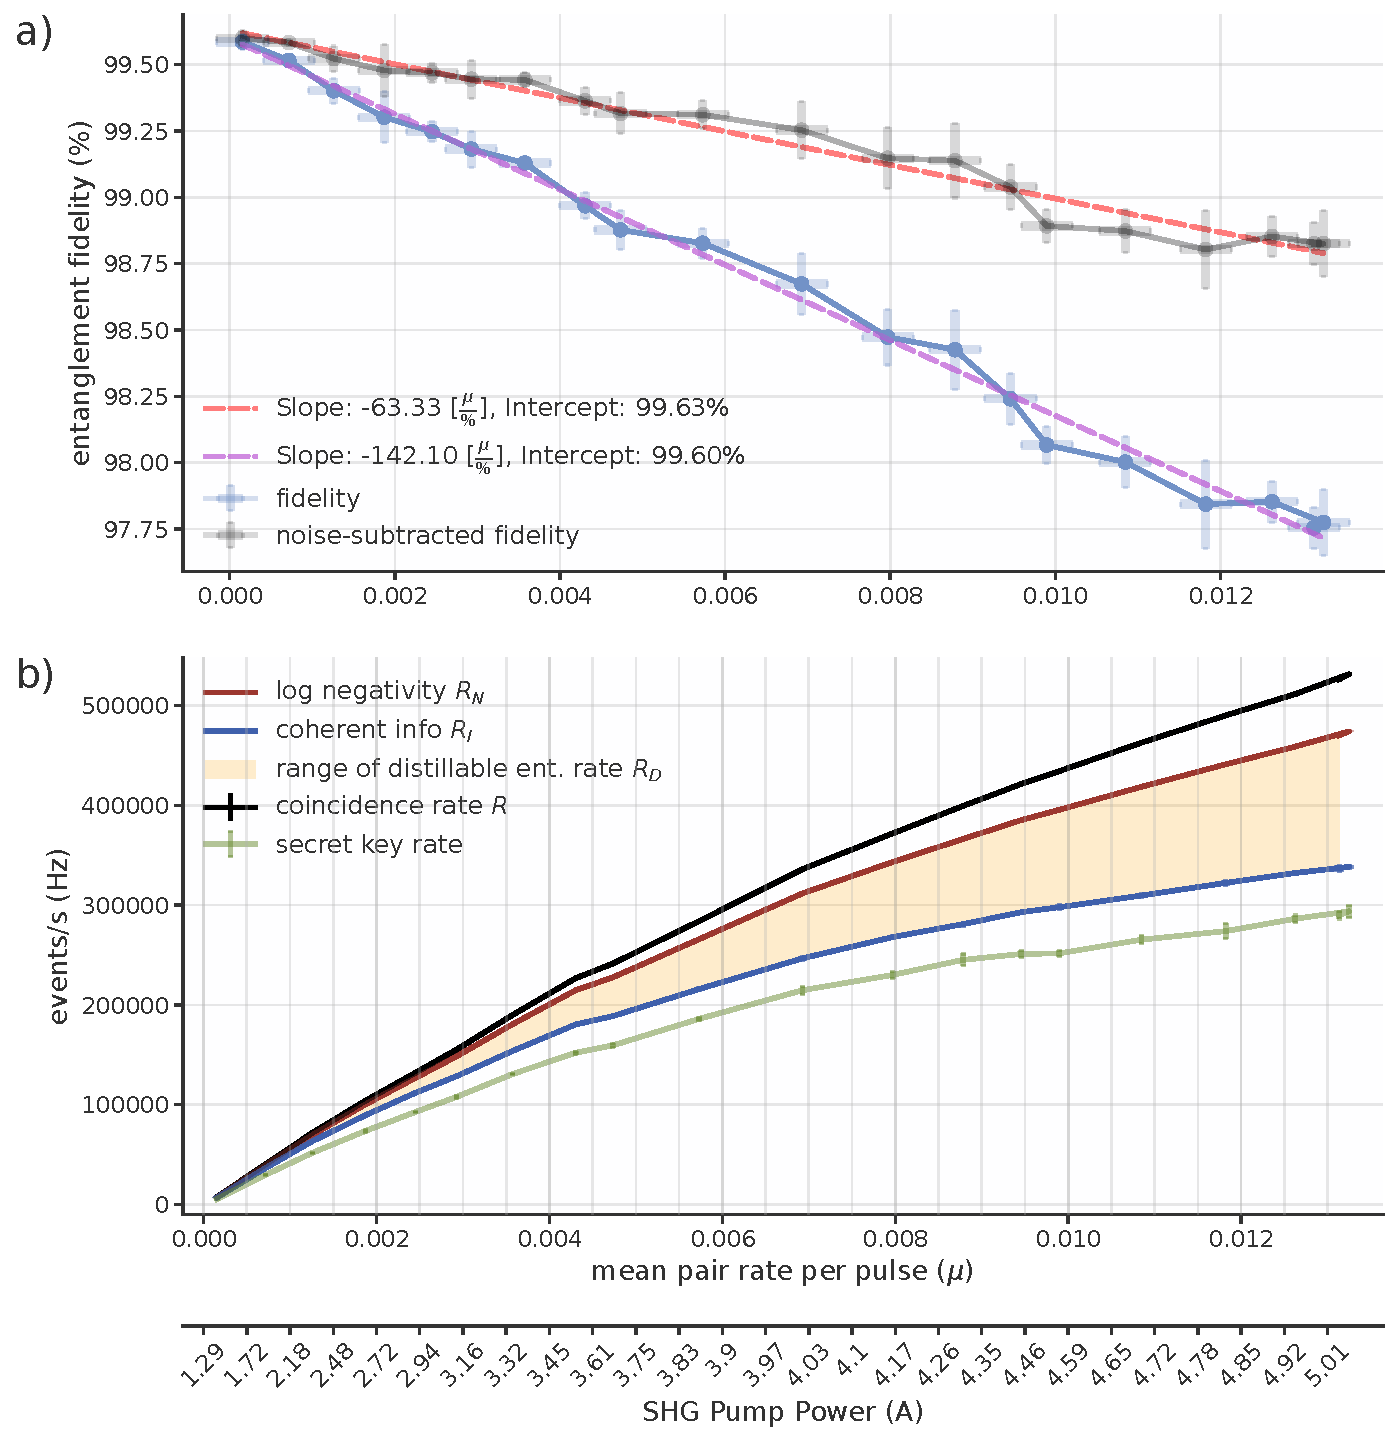
\includegraphics[width=0.8\textwidth,height=\textheight]{./chapter_05/figs/shg_scan_light.pdf}
\caption[{Entanglement visibility and rates vs pump power}]{\textbf{Entanglement visibility and rates vs pump power} a) Visibility versus pump power. Error bars are calculated by taking multiple measurements of the center bin coincidence rate over some integration time. These measurements span small ranges of interferometer phase, as the extremum-finding algorithm jitters the interferometer voltage. b) Bounded distillable entanglement rate versus pump power. Multiple such measurements are made for all the tomographic measurements. These are used to calculate standard deviations for visibility, log negativity, and coherent information. Error bars for the log negativity and coherent information are smaller than the line width shown. Rates shown assume readout of all 4 available interferometer ports, based on data measured using one port each at Alice and Bob.}
\label{fig:shg_scan}
\end{figure}
}

Due to the small size and temperature insensitivity of the interferometers, minimal temporal phase drift is observed over multiple hours. Nevertheless, software is used to lock the phase at a minimum or maximum with a simple hill-climbing algorithm. This varies the phase by small amounts over several minutes to search for or maintain an extremum.

Channels 35 and 59 are chosen for an analysis of entanglement visibility and rates versus pump power. Visibility with respect to pump power or mean entangled pair rate is shown in Fig.~\ref{fig:shg_scan} a. We define the entanglement visibility as $V = 100\%*(C_{max} - C_{min})/(C_{max} + C_{min})$ where $C_{min}$ and $C_{max}$ are the minimum and maximum coincidence rates in the middle bin for varied phase. As this coincidence rate depends on the total phase across the source and readout interferometers, only Bob's interferometer is actively controlled to scan the full state space.

The raw visibility versus $\mu$ is shown in blue in Fig.~\ref{fig:shg_scan} a. Relative to similar measurements \autocite{Kim2022}, this drops quickly with increasing $\mu$, and one reason is the presence of accidental coincidences across mutually incompatible spectral modes. The presence of these unwanted coincidences is a consequence of the narrowband filtering regime, and depends on factors included the singles rates $S_A$ and $S_B$, and the geometric compensation factor $\delta$ \textbf{\hl{(see Supplementary note 9 for derivation)}}. We model this type of accidental coincidence rate $C_{Acc}$ versus $\mu$, and subtract it off from coincidence measurements to produce the grey data in Fig.~\ref{fig:shg_scan} a. This simulated visibility's more gradual drop with increasing $\mu$ highlights the detrimental effect of our high single-to-coincidence rates $S_A/C_{AB}$, $S_B/C_{AB}$. As detailed in the discussion section below, this motivates special source engineering techniques for future systems.

\hypertarget{fig:channel_data}{%
\begin{figure}
\centering
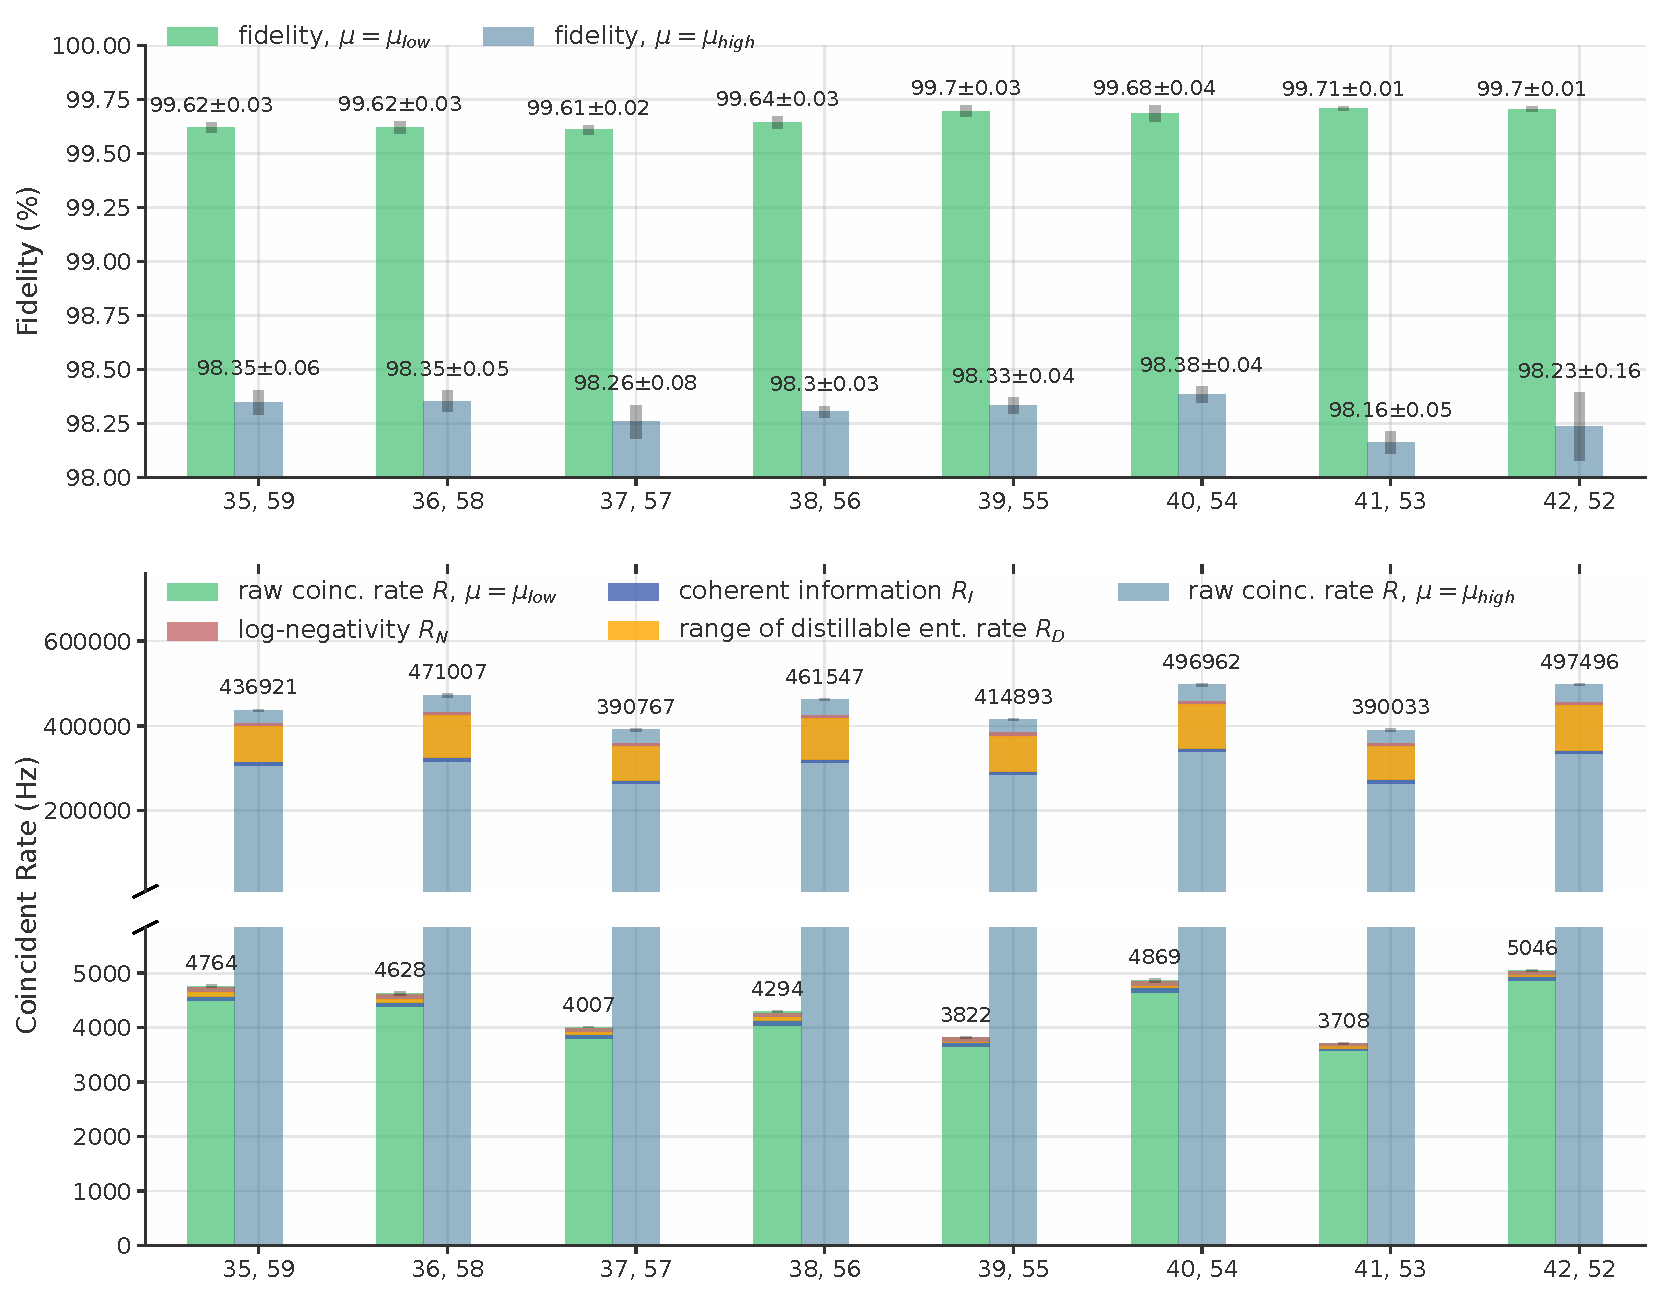
\includegraphics[width=0.8\textwidth,height=\textheight]{./chapter_05/figs/8ch_bar_graph_high_power_light.pdf}
\caption[{Visibilities and rates for 8 channel pairs}]{\textbf{Visibilities and rates for 8 channel pairs} a) Visibility for the main 8 channel pairs, measured at a high (22.9~mW) and a low (0.21~mW) SHG pump power setting. Each power setting results in similar $\mu$ for all channels: $\mu_L = 5.6{\times}10^{-5} \pm 9{\times}10^{-6}$ and $\mu_H = 5.0{\times}10^{-3} \pm 3{\times}10^{-4}$. b) Rate metrics for the 8 channel pairs at the same high and low power settings. The range of possible values for distillable entanglement rate is spanned by the yellow regions, bounded above by log-negativity and below by coherent information. Rates shown assume readout of all 4 available interferometer ports, based on data measured using one port each at Alice and Bob}
\label{fig:channel_data}
\end{figure}
}

We quantify the rate of useful entanglement by supplying bounds for the distillable entanglement rate $C_D$. Measured in ebits/s, $C_D$ is the maximal asymptotic rate of Bell-pair production per coincidence using only local operations and classical communications \autocite{Alshowkan2022,Bennett1996}. It is bounded above by log-negativity $C_N = C_{AB} E_N$ and below by coherent information $C_I = C_{AB} E_I$ \autocite{Alshowkan2022}. For each pump power setting in Fig.~\ref{fig:shg_scan}, a series of tomographic measurements is performed and density matrices are calculated. The values of $E_I$ and $E_N$ are calculated from the density matrices as detailed in \textbf{\hl{Supplementary note 8}}.

Figure Fig.~\ref{fig:channel_data} shows visibilities, raw coincidence rates, and bounded distillable entanglement rates for two pump powers and all 8 channel pairings. The highest pump power is currently limited by our EDFA-amplified SHG module. The pump power in principle could be increased until the SNSPD efficiency drops due to saturation, and the net coincidence rate plateaus. Without the time-walk correction, high-rate jitter becomes an issue well before the gradual drop of SNSPD efficiency. At the $\mu_H$ (22.9~mW) power, the singles rates $S_A, S_B$ average to 3.84 MHz, for which SNSPD efficiencies are about 78\% of nominal.

Using the data in Fig.~\ref{fig:figure_2nd_1} a, we model the JSI of our pair source as a product of pump envelope and phase matching condition functions

$$
|f(\omega_s, \omega_i)|^2 = |\psi_{\mathrm{ph}}\left(\omega_s, \omega_i\right)|^2 *|\psi_p\left(\omega_s, \omega_i\right)|^2,
$$

which depends on the wavelength (769.78 nm) and bandwidth (243 GHz FWHM) of up-converted light out of the SHG, measured with a spectrum analyzer. The path efficiencies from SPDC to detectors are also fitted based on integrations over the JSI that model the DWDM transmission passbands (\textbf{\hl{see Supplementary note 6}}).

We calculate the Schmidt decomposition of the pair source JSI, taking into account the DWDM filters at Alice and Bob, and derive an average inverse Schmidt number $1/K$ of $0.87$. This value quantifies the spectral purity of the entangled photon source, and is theoretically equivalent to the visibility of a two-source HOM (Hong-Ou-Mandel) interferogram~\autocite{mandel1995optical}. If 50 GHz ITU channels are used instead, the resulting filtered JSI better approximates a single mode, and the model predicts $1/K = 0.96$.

\hypertarget{discussion-1}{%
\section{Discussion}\label{discussion-1}}

\begin{table}
\begin{tabular}{ |p{3.5cm}||p{2.5cm}|p{2.5cm}|p{2.5cm}|p{2.5cm}|}
 \hline
 \multicolumn{5}{|c|}{Extrapolated rates (MHz)} \\
 \hline
 \makecell[l]{rate metric \\ ($\mu$ at max)}   &  1 Channel & 8 Channels & 16 Channels & 60 Channels \label{table:max_rates}\\
 \hline
 \makecell[l]{coincidence rate, $C_{AB}$ \\(0.014)} & 0.755 & 5.41    &  11.6  &  34.9     \\
 \hline
 \makecell[l]{log negativity, $C_N$ \\(0.010)}& 0.600 & 4.30    &  9.19  &  27.7   \\
 \hline
 \makecell[l]{coherent info., $C_I$ \\(0.006)}& 0.345 & 2.47 &  5.28  &  15.9 \\
 \hline
 \makecell[l]{secret key rate, $SKR$ \\(0.007)}& 0.309 & 2.21 &  4.73  &  14.3 \\
 \hline
\end{tabular}
\caption[{Extrapolating entanglement rates to more channels}]{Per-channel predicted maximum values for the 4 rate metrics are shown in the column labeled `1 Channel'. Depending on the metric, the maxima are achieved for different pump powers $\mu$ (See supplemental note 11). The $\mu$ value that maximizes each metric is shown in parenthesis on the left.}
\label{table:maximum_rates}
\end{table}

We have demonstrated that a time-bin entanglement source based on a mode-locked laser, spectral multiplexing and low-jitter detectors produces high entangled photon rates suitable for QKD or advanced quantum networks. Still, there is potential to increase rates beyond those measured here with some straightforward changes to the setup. First, a higher power EDFA-amplified SHG module or tapered amplifier may be used. With this, we predict a single channel pair could sustain rates up to those specified in the first column of Table 1. Our measurements of 8 channel and 16 channel configurations imply the approximately multiplicative scalings in columns 2 and 3, as coincidence rates of these channels pairs are all withing 27\% of each other. From measurements of the SPDC spectrum, it is also possible to extrapolate rates to a 60-channel 100 GHz DWDM configuration that includes channels spanning the L, C, and S ITU bands. This configuration could sustain 34.9 MHz total coincidence rate, and a distillable entanglement rate between 27.7 ($C_N$) and 15.9 Mebits/s ($C_I$). These rates are impressive considering they are achievable with existing SNSPDs and other technology. The SPDC spectrum and extrapolation details are found in \textbf{\hl{Supplementary note 11}}.

The ratio of singles rates $S_A, S_B$ to coincidence rates $C_{AB}$ are high in this system due to the relatively wide-band JSI and narrow filters. Each DWDM channel at Alice picks up a large fraction of photons that can't be matched with pairs passing though the corresponding channel passband at Bob, a feature quantified by the $\delta$ factor. The high singles rates lead to accidental coincidences from mutually incompatible spectral modes that lower visibility and load the detectors with useless counts. However, there is potential to mitigate these extra counts by embedding the nonlinear crystal undergoing SPDC in a cavity that enhances emission at the center frequencies of multiple DWDM channels~\autocite{Pomarico2009,Brydges2023,slattery2019background}. Also, there are other approaches to achieving such intensity islands that require dispersion engineering~\autocite{morrison2022frequency,xin2022spectrally}. With such periodically enhanced emission, the resulting JSI would exhibit a series of intensity islands lying along the energy-matching anti-diagonal, easily separable with DWDMs at Alice and Bob. The photon flux for each each channel would originate primarily from these islands covered by both signal and idler DWDM passbands, resulting in a higher ratio of coincidences to singles. The probability of accidental coincidences $C_{Acc}$ would be lower, and therefore bring the decrease of visibility with $\mu$ more in line with the modeled $V_C$ data in Fig.~\ref{fig:shg_scan}. Furthermore, this would enable substantially higher maximum rate metrics than those in table \ref{table:maximum_rates}.

This source is a fundamental building block for future space-to-ground and ground-based quantum networks. It leverages the strengths of the latest SNSPD developments -- namely simultaneous high count rates, low jitter and high efficiency -- and in doing so adopts interferometers and DWDM systems that are compact, stable and accessible. By elevating the system clock rate to 4.09 GHz and shrinking the time bin size to 80~ps, we have demonstrated a new state of the art in quantum communication that enables adoption of mature and extensively developed technologies from classical optical networks. Also, the spectral multiplexing methods used here are potentially compatible with those demonstrated in broadband quantum memories~\autocite{Sinclair2014} and optical quantum computing~\autocite{lukens2017frequency}.

\hypertarget{acknowledgements}{%
\subsubsection{Acknowledgements}\label{acknowledgements}}

Part of the research was carried out at the Jet Propulsion Laboratory, California Institute of Technology, under a contract with the National Aeronautics and Space Administration (NASA) (No.~80 NM0018D0004). Support for this work was provided in part by the Defense Advanced Research Projects Agency (DARPA) Defense Sciences Office (DSO) Invisible Headlights program, NASA SCaN, Alliance for Quantum Technologies' (AQT) Intelligent Quantum Networks and Technologies (INQNET) program, and the Caltech/JPL PDRDF program. A. M. is supported in part by the Brinson Foundation and the Fermilab Quantum Institute. M.S. is in part supported by the Department of Energy under Grant Nos. SC0019219 and SC002376. We are grateful to Si Xie (Caltech/Fermilab) and Cristi\{\textquotesingle{} a\}n Pe\{~ n\}a (Fermilab) for supporting this work in terms of sharing equipment and facilities. The authors acknowledge Prathwiraj Umesh for assistance in reviewing the manuscript.

\hypertarget{data-availability}{%
\subsubsection{Data availability}\label{data-availability}}

Data underlying the results presented in this paper are available in \autocite{mueller2023code,mueller2023data}.

\hypertarget{phase-basis-readout}{%
\section{Phase basis readout}\label{phase-basis-readout}}

This section uses numbers in kets to signify time delays, such that the notation from the main text transforms as $|e\rangle, |l\rangle \longrightarrow |0\rangle, |1\rangle$. Following the creation of the bell pair $\frac{1}{\sqrt{2}}(|00\rangle + e^{i \phi}|11\rangle)$ with the source interferometer, the readout interferometers at Alice and Bob transform each member of the entangled pair according to the operation \autocite{Marcikic2002}:

$$|k\rangle \rightarrow \frac{1}{2}\left(|k\rangle_{(A/B)+}+e^{i \phi_{s / i} \mid}|k+1\rangle_{(A/B)+}+i|k\rangle_{(A/B)-}-i e^{i \phi_{s / i}}|k+1\rangle_{(A/B)-}\right)$$

Where $(A/B)+$ and $(A/B)-$ denote the output ports of Alice ($A$) or Bob's ($B$) interferometer. The full state is a 28-term expression made of four so-called `branches' indexed by the four combinations of interferometer output ports: $A+ B+, A+ B- A- B+$ and $A- B-$. Each branch has a term in the following form, with amplitude dependent on the phase relationship between the interferometers:

$$p\left(e^{i \phi}+qe^{i\left(\phi_s+\phi_i\right)}\right)|2\rangle_{Au}|2\rangle_{Bv} $$

Where $p, q, u, v \in \{\{+1,+1, +, +\}, \{i,-1, +, -\}, \{i,-1, -, +\}, \{-1,+1, -, -\}\}$ for the four terms. These terms define the probability amplitude of the quantum state in the so-called phase basis. The modulous squared of these terms gives the phase-dependent probability of coincidences across the center time bins, as measured at interferometer outputs of Alice and Bob.

All the phase terms can be grouped into one variable $\theta = \phi_s + \phi_i - \phi$, and the four $|2\rangle|2\rangle$ terms can be re-expressed in terms of the the cosine function \autocite{Marcikic2002,Kim2022}:

\hypertarget{eq:cosines}{}{ 
\begin{align}
P_{A+ B+} &= |\langle 2|2\rangle|^2_{A+ B+} = 2(1 + v \cos(\theta)) \label{eq:cosines}\\
P_{A+ B-} &= |\langle 2|2\rangle|^2_{A+ B-} = 2(1 - v \cos(\theta)) \notag \\
P_{A- B+} &= |\langle 2|2\rangle|^2_{A- B+} = 2(1 - v \cos(\theta)) \notag \\
P_{A- B-} &= |\langle 2|2\rangle|^2_{A- B-} = 2(1 + v \cos(\theta)) \notag \\ \notag
\end{align}
}

where $v$ was added to denote the visibility of the phase basis. Scanning the phase of the system and measuring coincidence rate across the center bins produces sinusoidal fringes as shown in Fig.~\ref{fig:fringes}.

\hypertarget{coincidence-rate-interferometer-output-ports}{%
\section{Coincidence Rate \& Interferometer Output Ports}\label{coincidence-rate-interferometer-output-ports}}

As each readout interferometer has two output ports, the full output state observed at Alice and Bob cannot be fully measured with two SNSPDs. We label the output ports of Alice (A) and Bob's (B) interferometers with plus ($+$) and minus ($-$). The plus ports are used for most measurements. By measuring the relative loss between the plus and minus ports, all singles rates $S_i$ and coincidence rates $C_{ij}, i,j \in \{A+, A-, B+, B-\}$ across different detectors can be estimated.

$R_A$ is the ratio of transmissions $t_{A-}$ over $t_{A+}$, where $t_{A-}$ is the transmission through the input to output $A-$ and $t_{A+}$ is the transmission through the input to output $A-$. $R_B$ is defined analogously. We measure values for $R_A$ and $R_B$ by sending a pulsed laser into the input and measuring the ratio of power transmitted across the output ports:

$$R_A = 0.99 \pm 0.03, ~~~~~~ R_B = 1.04 \pm 0.03$$

\hypertarget{fig:branches}{%
\begin{figure}
\centering
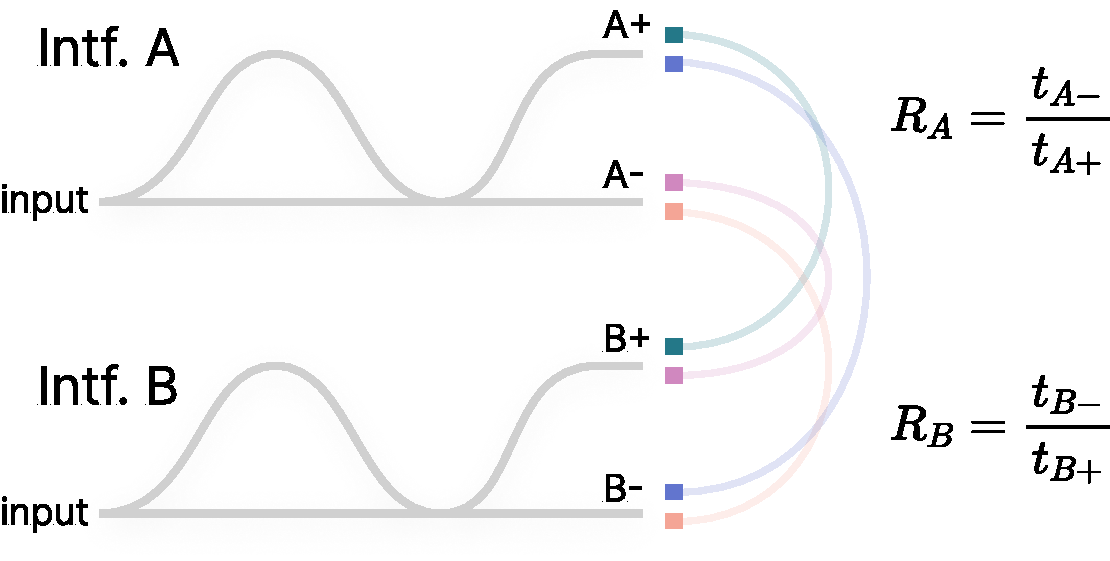
\includegraphics[width=0.7\textwidth,height=\textheight]{./chapter_05/figs/branches_light.pdf}
\caption[{Wavefunction branches}]{\textbf{Wavefunction branches} Different pairings of interferometer output ports collect different wavefunction branches}
\label{fig:branches}
\end{figure}
}

The coincidence rates for all wavefunction branches are the same if $\theta$ in Eq.~\ref{eq:cosines} is set to zero. With this phase state rate $C_{A+ B+, \theta=0}$ measured directly (labeled B in Fig.~\ref{fig:fringes}), it's straightforward to estimate the full wavefunction coincidence rate across all interferometer outputs. As shown in table \textcite{table:rates}, the rate is $C_{A+ B+}(1 + R_A + R_B + R_AR_B)$. This estimate is used to express a full coincidence rate for figures 3 and 4 in the main text.

\definecolor{color1}{HTML}{38A5BA}
\definecolor{color2}{HTML}{6275CE}
\definecolor{color3}{HTML}{D088BF}
\definecolor{color4}{HTML}{F4A596}
\begin{table}
\label{table:branches}
\begin{tabular}{ |p{2.5cm}||p{1.3cm}|p{2.9cm}|p{2.9cm}|p{3.4cm}|  }
\hline
\multicolumn{5}{|c|}{Predicted Singles and Coincidence Rates for Full Wavefunction} \\
\hline
rate metrics     &  Branch 1 & Branch 2 & Branch 3 & Branch 4 \label{table:rates}\\
\hline
singles rate 1  & $S_{A+}$ &$S_{A-}=R_A S_{A+}$    &$S_{A+}$               &$S_{A-}=R_A S_{A+}$        \\
singles rate 2  & $S_{B+}$ &$S_{B+}$               &$S_{B-} = R_B S_{B+}$  &$S_{B-} = R_B S_{B+}$      \\
coincidence rate&\textcolor{color1}{$C_{A+B+}$}&\textcolor{color3}{$C_{A-B+}=R_A C_{A+B+}$}&\textcolor{color2}{$C_{A+B-}=R_B C_{A+B+}$}&\textcolor{color4}{$C_{A-B-}=R_B R_A C_{A+B+}$}\\
\hline
\end{tabular}
\caption[{Rates for wavefunction branches}]{Singles and coincidence rates for wavefunction branches. The $A+, B+$ branch was measured, and the rates of other branches are predicted using relative transmission factors $R_A, R_B$}
\end{table}

For main-text figure 2 in particular, coincidences were measured with the center bin rate tuned to a minimum $\theta=-\frac{\pi}{2}$ (grey solid line in main-text figure 2c). The rate therefore captures the contribution from the 6 phase-independent terms for the $A\!\!+\!\!B\!+\!$ wavefunction branch. This can be extrapolated to the $\theta=0$ state by multiplying by $\frac{4}{3}$. For the rate displayed to be consistent with the measures of coupling efficiency $\eta$ (and so the interferometers aren't thought of as a source of $\sim$ 50\% loss), this rate is multiplied again by $(1 + R_AR_B)$ to represent two wavefunction branches. This results in a total scaling of:

$$C_{fig. 2} = \frac{4}{3}(1 + R_AR_B)C_{measured}$$

\hypertarget{joint-spectral-intensity-analysis}{%
\section{Joint Spectral Intensity Analysis}\label{joint-spectral-intensity-analysis}}

This entanglement source is potentially useful for future quantum communication systems that make use of two-photon interference, such as teleportation or entanglement swapping. These require the generation of highly pure and indistinguishable photons. The type-0 SPDC crystal used in this source shows strong spectral correlations that make it inappropriate for two-photon interference demonstrations by itself. However, with the application of the DWDM filtering, we create a series of spectral channel pairings that are potentially good individual sources of fairly pure single mode photons. To investigate this, we model the joint spectral intensity function (JSI) produced by the SPDC and fit it to data. Then we and apply a Schmidt decomposition to the spectral modes produced when pairs of DWDM filter channels are applied to the modeled JSI. We derive an inverse Shmidt number which is equal to single photon purity $P$ as well as visibility $V$ of Hong-Ou-Mandel (HOM) interference. An inverse Schmidt number approaching 1 indicates that the source is effective for two-photon interference measurements like HOM and Bell State measurements.

\hypertarget{jsi-modelling}{%
\subsection{JSI modelling}\label{jsi-modelling}}

We follow an analysis for co-linear quasi-phase matching inside a waveguide packaged SPDC crystal \autocite{Davis2022,ZielnickiKwiat2018SPDCmodel}. The joint spectral intensity $|f(\omega_s, \omega_i)|^2$ is modelled as a product of phase matching and pump envelope intensities \textbar{}$\psi_{\mathrm{ph}}\left(\omega_s, \omega_i\right)|^2$ and $|\psi_p\left(\omega_s, \omega_i\right)|^2$, where $\omega_s$ and $\omega_i$ are the frequencies of the signal and idler models respectively. The phase matching envelope intensity takes the form:

$$
\left|\psi_{\mathrm{ph}}\left(\omega_s, \omega_i\right)\right|^2=\operatorname{sinc}^2\left(\frac{\Delta k L}{2}\right),\;\;\;\;\;\; \Delta k=2 \pi\left(\frac{n\left(\lambda_p\right)}{\lambda_p}-\frac{n\left(\lambda_s\right)}{\lambda_s}-\frac{n\left(\lambda_i\right)}{\lambda_i}-\Gamma\right)
$$

where $L$ is the length of the crystal, $\Delta K$ is a wave-vector mismatch term, and $n_{p(s)(i)}$ is the refractive index of the crystal at the wavelengths of pump $\lambda_p$, signal $\lambda_s$ and idler $\lambda_i$. $\Gamma = 1/\Lambda$ where $\Lambda$ is the polling period of the crystal. The refractive indices $n(\{\lambda_p, \lambda_s, \lambda_i\})$ are computed from an MgO-doped PPLN Sellmeier equation \autocite{Gayer2008}. In the expression for $\Delta K$, $\lambda_p$ is the function of $\lambda_s$ and $\lambda_i$ that imposes energy conservation: $1/\lambda_p = 1/\lambda_s + 1/\lambda_i$.

The pump envelope intensity is modeled as

$$|\psi_p\left(\omega_s, \omega_i\right)|^2=\exp \left(-\frac{\left(\omega_p-\omega_s-\omega_i\right)^2}{\sigma_p^2}\right)$$

where $\omega_p$ and $\sigma_p$ are the center frequency and bandwidth of the pump signal out of the EDFA/SHG module. Unlike $\lambda_p$ in the phase matching expression above, $\omega_p$ and $\sigma_p$ are fixed to known values or chosen as floating fitting parameters.

\hypertarget{jsi-fitting}{%
\subsection{JSI fitting}\label{jsi-fitting}}

The JSI model is fitted to the the 8x8 DWDM data from Fig.\textasciitilde2a in the main text. The transmission spectrum of one DWDM channel was measured and used to estimate the transmission properties for all pairs of 8 channels. For each measurement of coincidence rate from Fig.\textasciitilde2a we define an integration over the joint spectral intensity and the corresponding filter passbands:

\hypertarget{eq:c_uv}{}{
\begin{align}
    C_{u,v} = \int_{s}\int_{i}T_u(\lambda_s)T_v(\lambda_i)|f(\omega_s, \omega_i)|^2 d\lambda_s d\lambda_i \label{eq:c_uv}
\end{align}
}

where $T_{u(v)}$ is the transmission spectrum for filter with ITU channel $u (v)$, and the integrations are over the signal and idler wavelengths. Efficiency parameters $\eta_i$ scale the DWDM filter spectrums, and are used to model all loss between pair generation in the SPDC crystal and detection in the SNSPDs. To fit the $\eta_i$ values, the singles rates from Fig.\textasciitilde2a were also included, and fitted to single-filter integrations:

$$S_{u} = \int_{s}\int_{i}T_{u}(\lambda_a)|f(\omega_s, \omega_i)|^2 d\lambda_s d\lambda_i$$

Where $a \in \{i, s\}$. Parameters of model for $|f(\omega_s, \omega_i)|^2$ were optimized to minimize the error between estimates $C_{u,v}$ and $S_u$ and the measured coincidence and singles rates. The following parameters were either set explicitly based on measurements and known constants (black), or optimized in the fitting process (blue):

\hypertarget{fig:parameters}{%
\begin{figure}
\centering
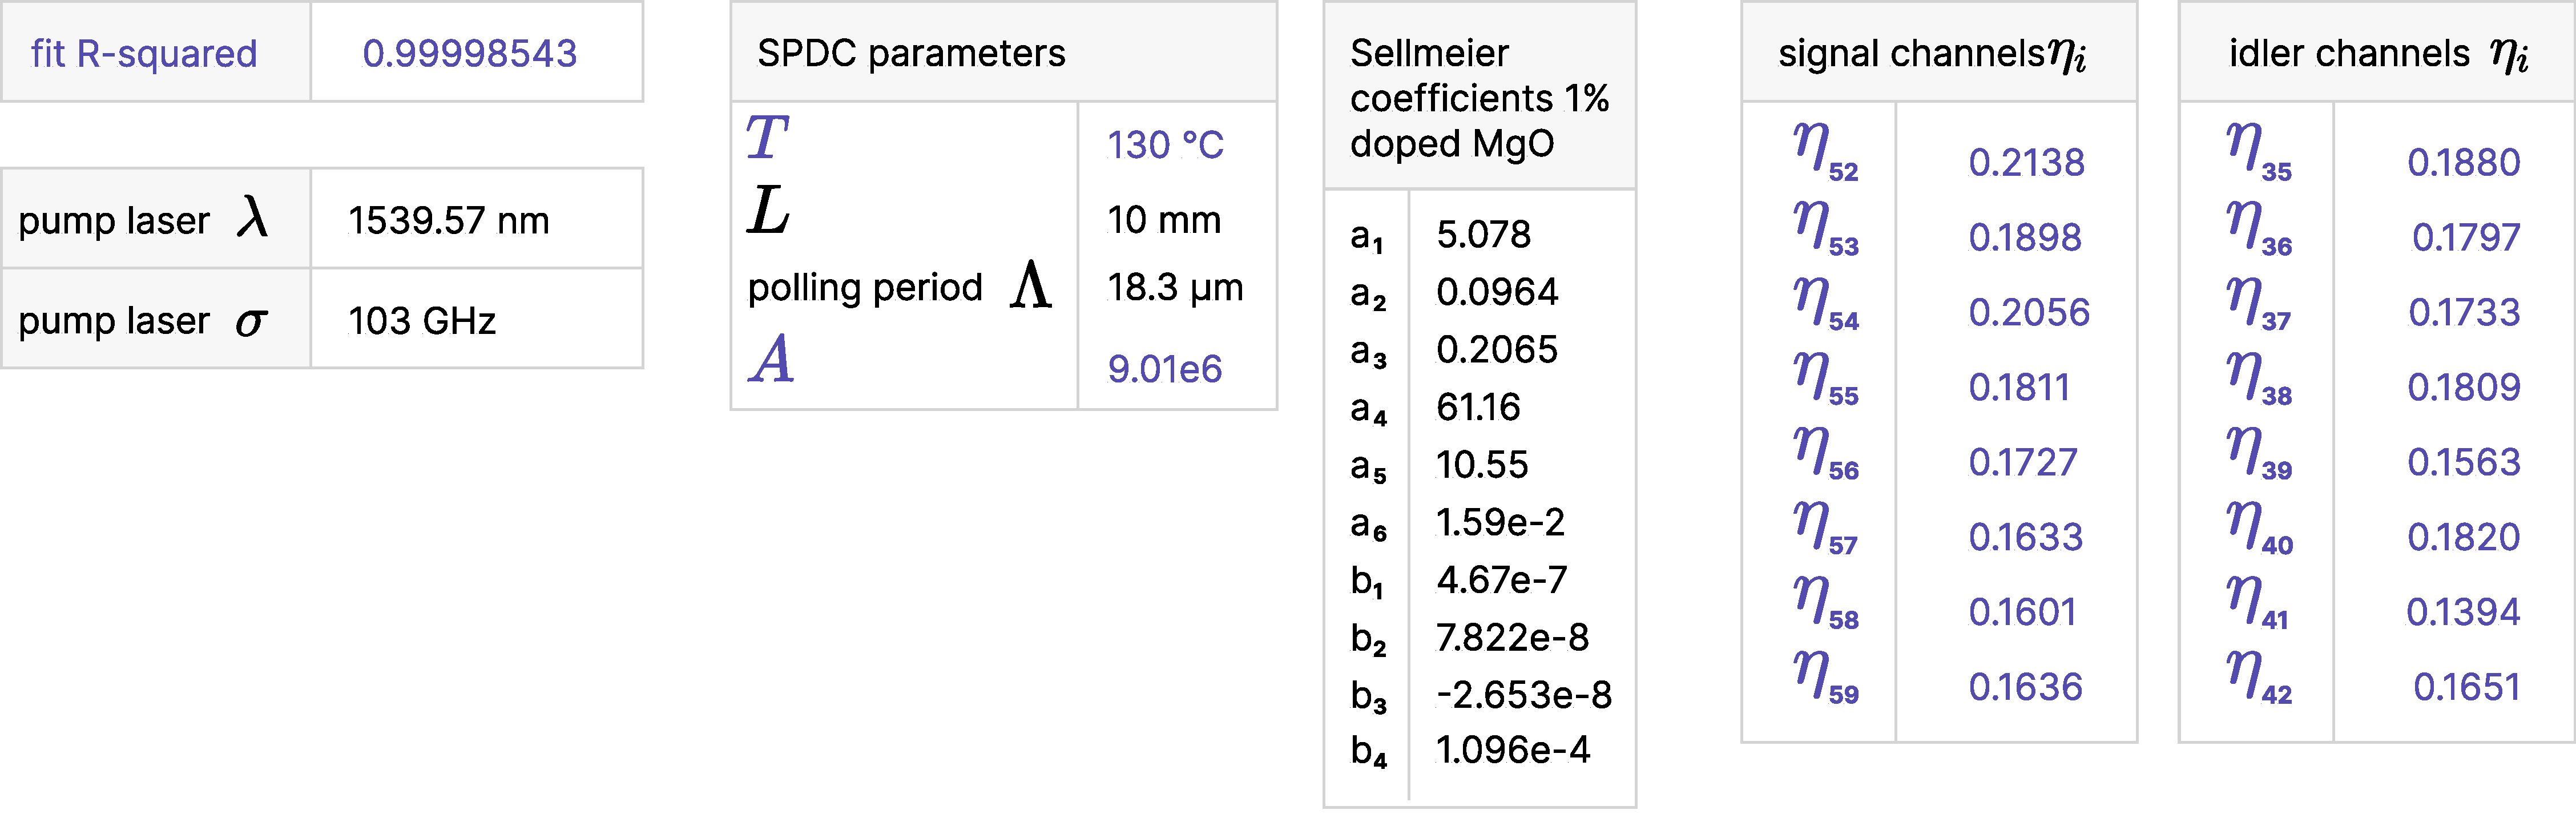
\includegraphics[width=1\textwidth,height=\textheight]{./chapter_05/figs/fitting_parameters_light.pdf}
\caption[{JSI fitting parameters}]{\textbf{JSI fitting parameters} Pump laser $\lambda$ and $sigma$ were found by measuring the output of the SHG module with a spectrum analyzer.}
\label{fig:parameters}
\end{figure}
}

Varying MgO doping percentage and varying crystal temperature affect the Sellmeier equations in similar ways \autocite{Gayer2008,Jundt1997}. Therefore, crystal temperature $T$ was used as a fitting parameter, to stand in the unknown MgO doping percentage. The true crystal temperature during all measurements was $50.0^{\circ}~\mathrm{C}$, which was optimized to maximize coincidence rates.

\hypertarget{fig:jsi_sim}{%
\begin{figure}
\centering
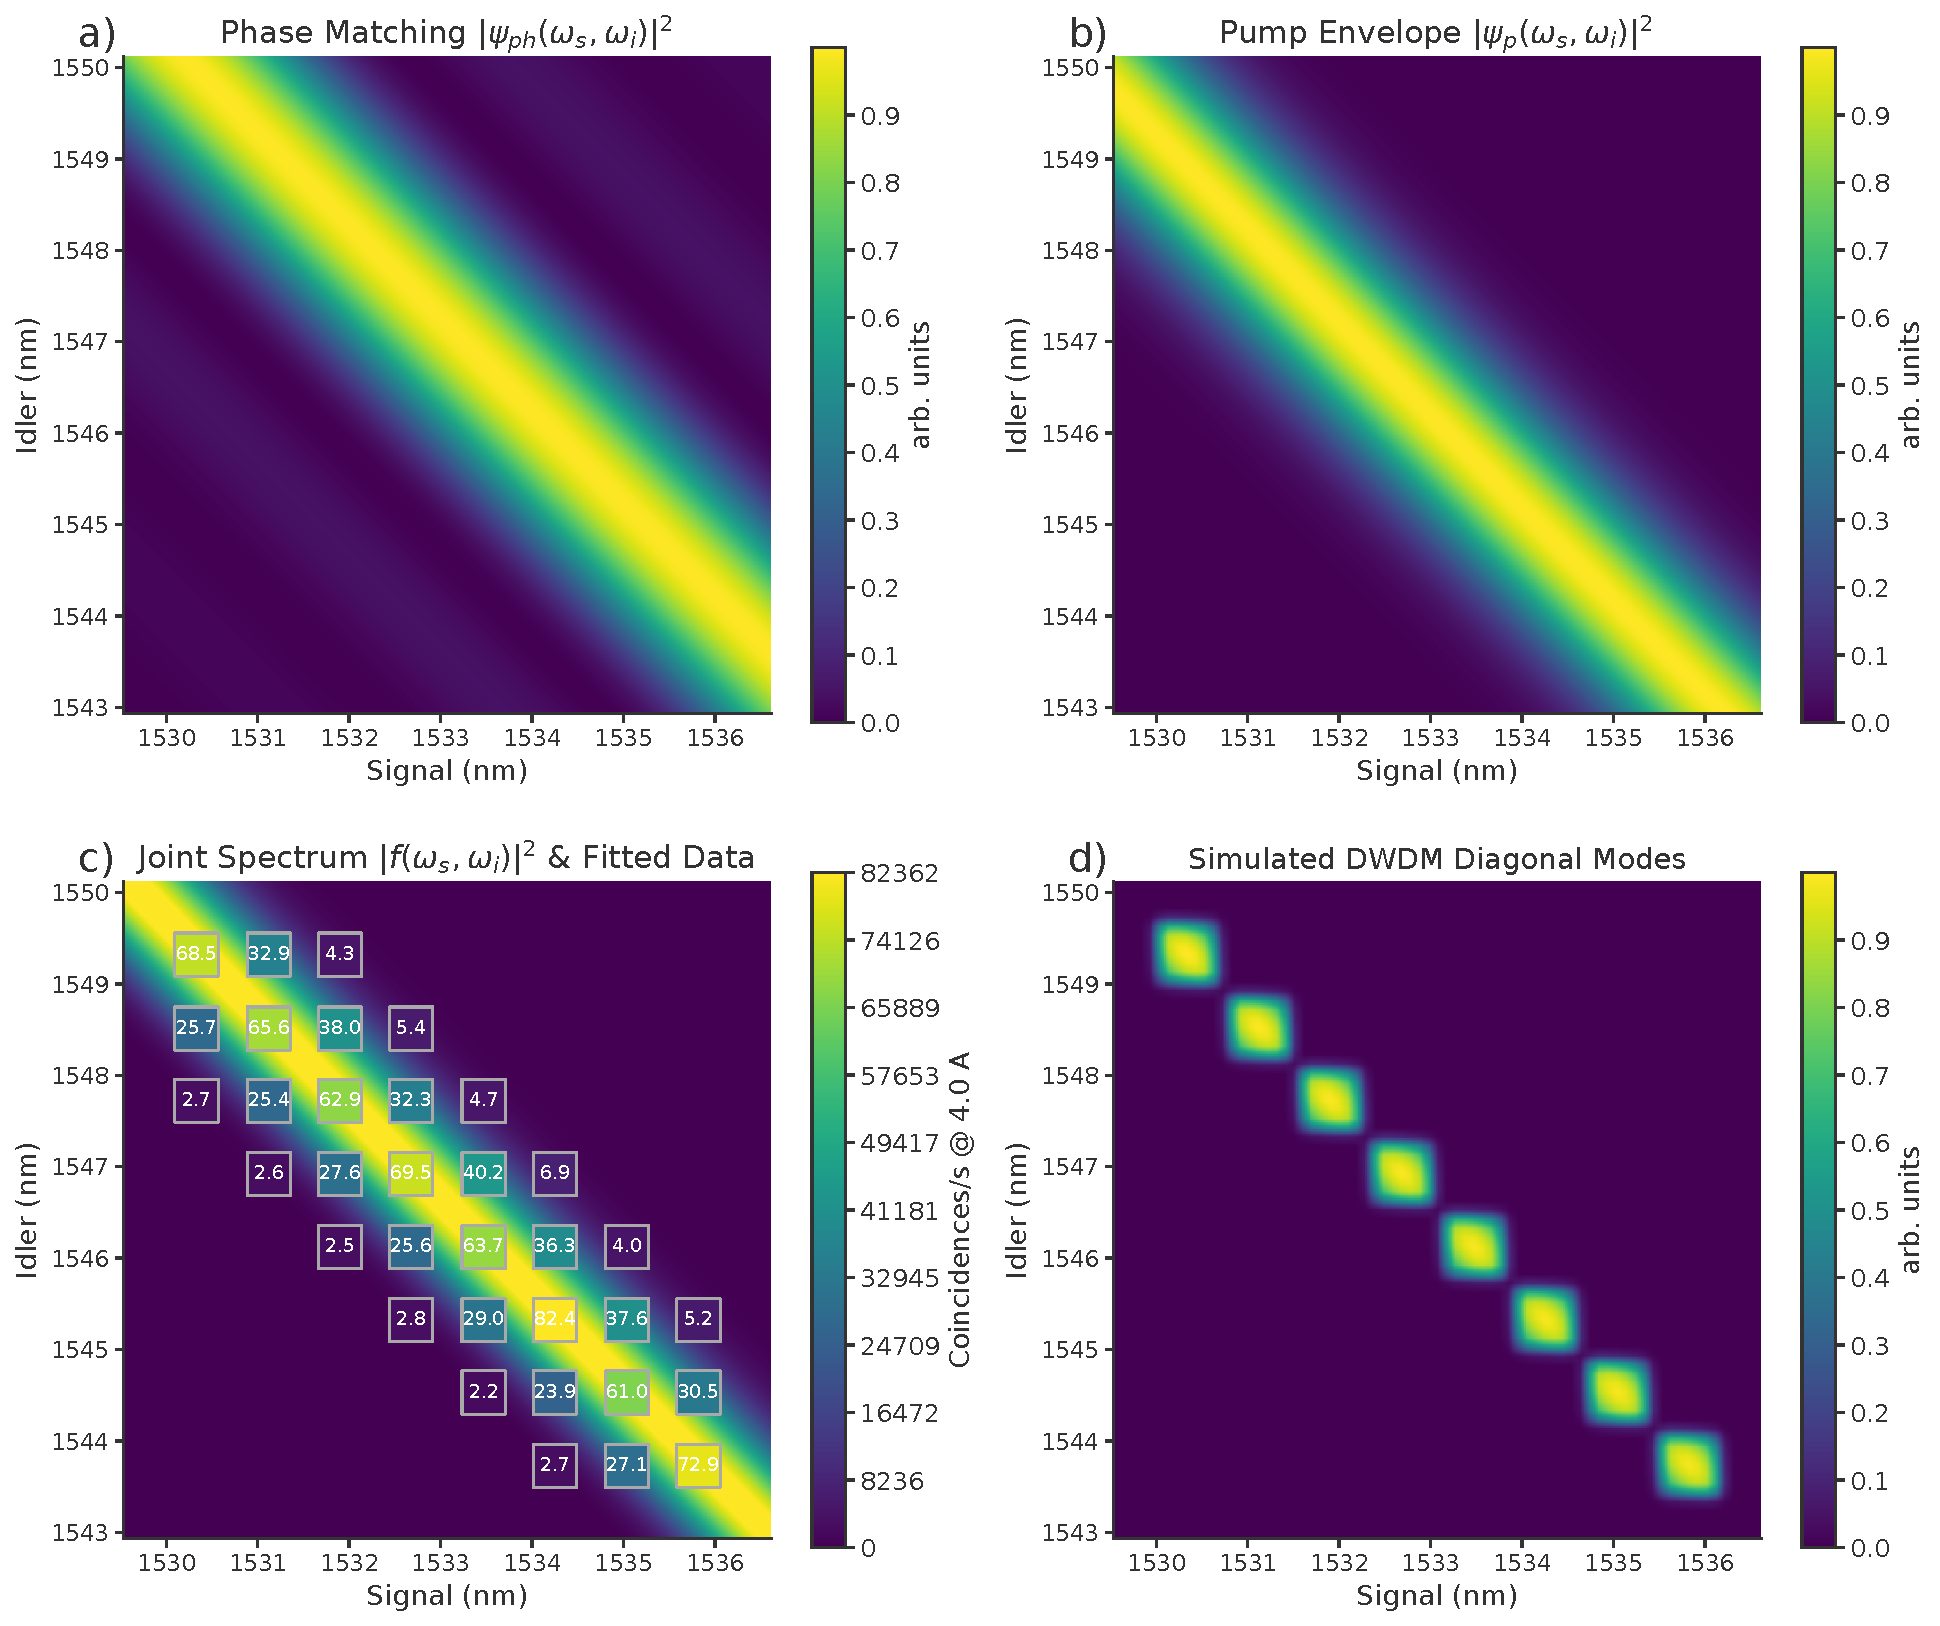
\includegraphics[width=1\textwidth,height=\textheight]{./chapter_05/figs/JSI_sim_results_light.pdf}
\caption[{JSI simulation results}]{\textbf{JSI simulation results} a) \& b) For type-0 SPDC, the relationship between refractive indices of pump and down-converted wavelengths produces an intensity profile roughly parallel with the pump envelope. This is responsible for the broad output spectrum of these crystals. c) the coincidence rates in Kcounts/s that are fit to filter-defined integrations of the JSI. d) Joint spectral distributions of coincidences expected from the filter pairings that correspond to the main diagonal. Here the joint spectrums of 8 DWDM channels pairs are shown summed together, where each component of the sum is an expression like the integrand of $C_{u,v}$ above.}
\label{fig:jsi_sim}
\end{figure}
}

An ideal photon pair source for scalable optical quantum information processing would not exhibit joint spectral correlations between the signal and idler photons. The Schmidt decomposition, which is equivalent to the singular value decomposition in our computational model, can be used to quantify these correlations \autocite{ZielnickiKwiat2018SPDCmodel}. We apply the Schmidt decomposition to the filtered JSIs for filter pairings along the main diagonal in Fig.\textasciitilde2a in the main text, and derive the inverse Schmidt number for these modes

$$1/K = \sum_i \lambda_i^2$$

where $\lambda_i$ are the Schmidt coefficients \autocite{ZielnickiKwiat2018SPDCmodel}. The inverse Schmidt numbers for all 8 channel pairs are similar, and are not expected for vary due to any phenomena beyond inaccuracies of the model. Therefore, we quote single values for $1/K$ in the main text.

\hypertarget{consequences-of-narroband-filtering}{%
\section{Consequences of Narroband Filtering}\label{consequences-of-narroband-filtering}}

\hypertarget{calculation-of-mean-photon-number-per-pulse-ux3bc}{%
\subsection{\texorpdfstring{Calculation of mean photon number per pulse \texorpdfstring{$\mu$}{mu}}{Calculation of mean photon number per pulse }}\label{calculation-of-mean-photon-number-per-pulse-ux3bc}}

\hypertarget{fig:narroband}{%
\begin{figure}
\centering
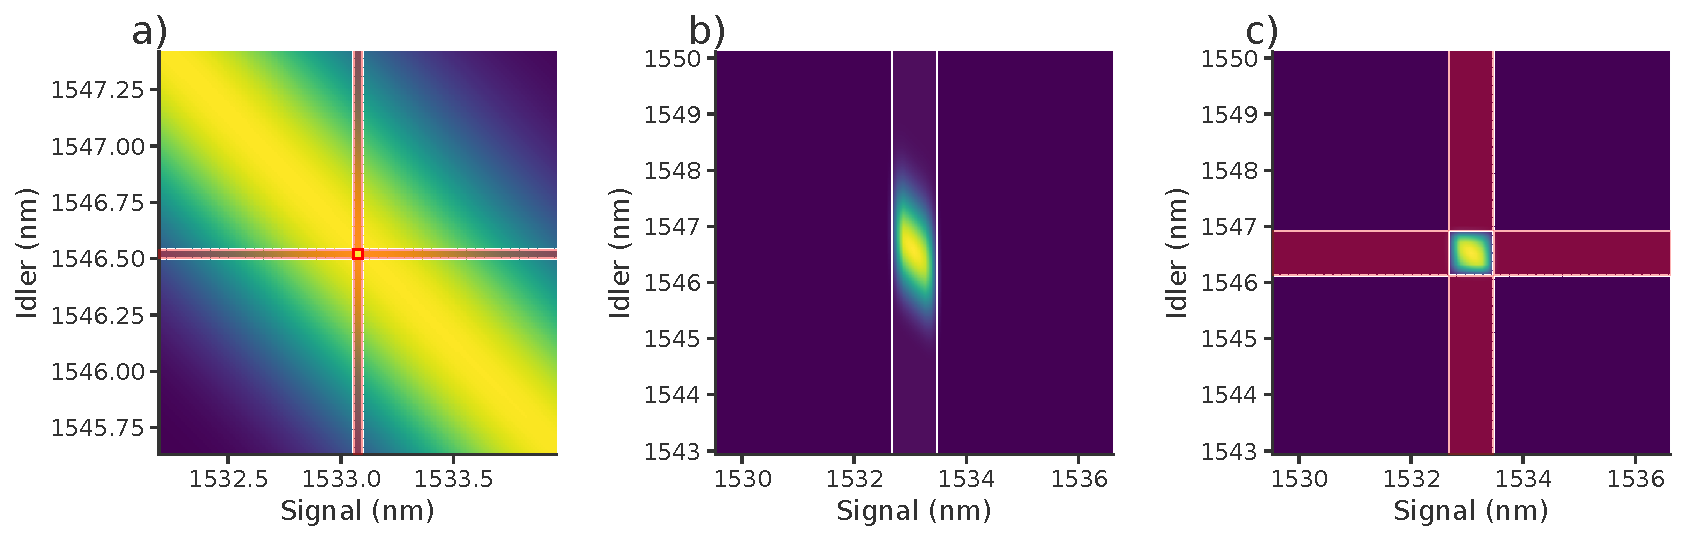
\includegraphics[width=1\textwidth,height=\textheight]{./chapter_05/figs/filter_considerations_light.pdf}
\caption[{JSI filtering considerations}]{\textbf{JSI filtering considerations} a) Two filters with bandwidth approximately 0.04 nm are applied to the JSI model. True coincidences are expected only from the region inside the small red square. b) The shape of the JSI with one 100 GHz DWDM filter applied c) the JSI a 100 GHz DWDM filter applied on both signal and idler arms.}
\label{fig:narroband}
\end{figure}
}

It is common in the literature to calculate signal and idler arm efficiencies with equations of the form:

\hypertarget{eq:regular_eff}{}{
\begin{align}
\eta_{s(i)}=\frac{C_{s i}}{S_{i(s)}} \label{eq:regular_eff}
\end{align}
}

Where $\eta_{s(i)}$ is coupling efficiency of the signal (idler) arm, $C_{s i}$ is the coincidence rate, and $S_{i(s)}$ is the singles rate on the idler (signal) arm. $\mu$, the mean pair rate per period or cycle, may also be defined in terms of the repetition rate $R$ as $R \mu \eta_{s(i)}=S_{s(i)}$. With these, one can define $\mu$ in terms of coincidence rate $C_{s i}$ and singles rates $S_s$ and $S_i$:

\hypertarget{eq:colorless}{}{
\begin{align}
    \mu=\frac{S_s S_i}{C_{s i} R} \label{eq:colorless}
\end{align}
}

However, this definition breaks down in the limit of narroband filtering, or when the losses on the signal and ider arm cannot be thought of as `colorless'. Consider the situation of two very-narroband filters, as illustrated in figure Fig.~\ref{fig:narroband} a. This situation can be simulated using the JSI model. We set signal and idler filter bandwidth to 5\% of the 100 GHz DWDM bandwidths. Pump power is scaled by 200x. Transmission of the filters at their maximum is set to 100\%. This results in $S_s = 58.0~\mathrm{MHz}$, $S_i = 57.6~\mathrm{MHz}$, and $C_{s i} = 567~\mathrm{KHz}$. With these values, Eq.~\ref{eq:colorless} suggests a $\mu$ value of 1.47. This is misleading because it's unreasonable to expect the red outlined region at the intersection of the filters in Fig.~\ref{fig:narroband} a --which is responsible for all true detections of entangled pairs-- to be the source of more than one entangled pair per pulse. Rather, the high singles rates $S_s$ and $S_i$ are having an adverse effect on the $\mu$ calculation. Most of the singles detections are from mutually incompatible spectral modes -- the 4 regions that form a cross shape above, below, and to the sides of the red outlined square.

We propose a definition of $\mu$ similar to the form of Eq.~\ref{eq:c_uv}:

\hypertarget{eq:newmu}{}{
\begin{align}
    \mu_{u,v} = \frac{1}{R}\int_{s}\int_{i}W_u(\lambda_s)W_v(\lambda_i)|f(\omega_s, \omega_i)|^2 d\lambda_s d\lambda_i \label{eq:newmu}
\end{align}
}

where $W_u$ and $W_v$ have the spectrums of filters $T_u$ and $T_v$ but maximum transmissions of 100\%. This is an integration of $|f(\omega_s, \omega_i)|^2$ over the bipartite spectral region where filter transmission is non-negligible. As the JSI model is defined, $|f(\omega_s, \omega_i)|^2$ has units of entangled pairs per $\mathrm{nm}^2$.

Going forward, we use the Eq.~\ref{eq:newmu} definition of $\mu$ in the main text, and do a separate analysis of the effect of the mutually incompatible spectral modes when necessary. Note that in the main text, Alice receives idler photons and Bob receives signal photons, so variables transform as $C_{is} \rightarrow C_{AB}$, $S_{i} \rightarrow S_{A}$, and $S_{s} \rightarrow S_{B}$

\hypertarget{estimating-ux3bc-from-coincidence-and-singles-rates}{%
\subsection{\texorpdfstring{Estimating \texorpdfstring{$\mu$}{mu} from coincidence and singles rates}{Estimating  from coincidence and singles rates}}\label{estimating-ux3bc-from-coincidence-and-singles-rates}}

As Eq.~\ref{eq:colorless} is problematic for the narroband filtering regime, a conversion is needed that maps this type of expression to the more implicitly defined Eq.~\ref{eq:newmu}. Luckily, the influence of narroband filtering as a sort of pseudo-loss can be rolled into a new geometric factor $\delta$. This is the ratio of the JSI captured by two narroband spectral filters $W_u(\lambda_s)*W_v(\lambda_i)$ to that captured by one $W_v(\lambda_i)$, as illustrated in Fig.~\ref{fig:narroband} b and c.~Consider an expression for $\delta$ in terms of measured and fitted quantities:

\hypertarget{eq:new_eff}{}{
\begin{align} 
\delta_{i(s)} = \frac{C_{is}}{\eta_{i(s)}S_{s(i)}} \label{eq:new_eff}
\end{align}
}

Here, $S_{s(i)}$ is the singles rate through a signal (idler) narrowband filter. $\eta_{i(s)}S_{s(i)}$ would be the coincidence rate if the idler (signal) filter was wide-band (or just colorless loss), but maintained the same efficiency as measured ($\eta_{i(s)}$). Therefore the fraction can be thought of as the ratio of a coincidence rate measurement with two narroband filters $[C_{is}]$ to a coincidence rate measurement with one narro-band and one wide-band filter $[\eta_{i(s)}S_{s(i)}]$. As we use the same bandwidth filters on the signal and idler arms, the $\delta_i$ and $\delta_s$ calculated from the measured data and JSI fitting results are similar. We use an averaged single $\delta$ value for all further analysis, unique to our JSI bandwidth and 100 GHz DWDM filters.

$$\delta = 0.393 \pm 0.012$$

This is averaged from 8 $\delta_i$ and 8 $\delta_s$ values, for the 8 DWDM channel pairs along the main diagonal of the JSI.

We see Eq.~\ref{eq:new_eff} is a modified form of Eq.~\ref{eq:regular_eff} that includes $\delta$. With $R \mu \eta_{s(i)}=S_{s(i)}$ again, we can define a new expression for $\mu$ using singles $S_{s(i)}$ and coincidence $C_{is}$ rates.

\hypertarget{eq:new_mu}{}{
\begin{align}
    \mu = \frac{\delta S_s S_i }{R C_{is}} \label{new_mu}
\end{align}
}

This is used to compute $\mu$ in the main text.

\hypertarget{quantum-state-tomography}{%
\section{Quantum State Tomography}\label{quantum-state-tomography}}

We perform quantum state tomography of individual channel pairs in order to resolve the full density matrix and calculate bounding terms for the distillable entanglement rate.

Established methods for tomography of time-bin entangled photon pairs involve independent phase control of the two readout interferometers. However, the center bin coincidence rate depends on an overall phase which is the sum of source and readout interferometer phases (see Eq.~\ref{eq:cosines}). By manipulating the overall phase through control of only one interferometer, we assume that the full phase-dependent behavior of the system is captured. The data for the tomography is captured with Alice's interferometer in 3 phase settings. That which minimizes coincidence rate of the center bin (labelled A in Fig.~\ref{fig:fringes}), that which maximizes coincidences in the center bin (C), and a state halfway between in phase (B). The (B) state is chosen by setting the interferometer power to a value halfway between the power settings for states A and C. We therefore assume phase scales linearly with power, which is supported by the good agreement in Fig.~\ref{fig:fringes} between the phase fringes and a cosine fit.

\hypertarget{fig:fringes}{%
\begin{figure}
\centering
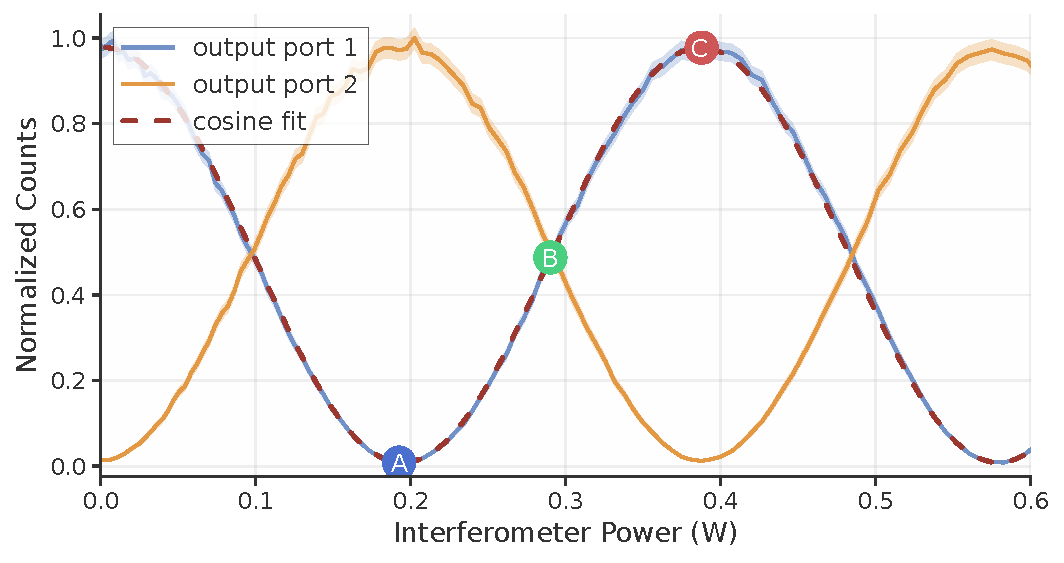
\includegraphics[width=0.9\textwidth,height=\textheight]{./chapter_05/figs/fringes_light.pdf}
\caption[{Center bin fringe measurement}]{\textbf{Center bin fringe measurement} Coincidence rate across center time bin with respect to interferometer power. The fringe data was measured for the two output ports of Alice's interferometer. The output port 1 data was fitted to a cosine curve using linear least squares.}
\label{fig:fringes}
\end{figure}
}

Multiple measurements involving all three time bins are performed with the phase set in these 3 states. The columns labeled A, B, and C in Fig.~\ref{fig:counts_chart} correspond to these 3 measurement conditions, where the measurements for the 90 degree phase measurements are repeated in columns 2 and 3. We organize the coincidence data in this format to show how it relates to more canonical constructions of tomography data where the phases of the two readout stations are controlled independently \autocite{Zhang2021Tomography,Takesue09Tomography}. Summing the counts in each row yeilds a 16-element vector which is sufficient to calculate a density matrix using a maximum likelyhood method \autocite{tomography2023}.

\hypertarget{fig:counts_chart}{%
\begin{figure}
\centering
\includegraphics[width=1\textwidth,height=\textheight]{./chapter_05/figs/chart_1_light.pdf}
\caption[{Quantum state tomography measurements}]{\textbf{Quantum state tomography measurements} Quantum state tomography data for one low-power (SHG at 1.2 Amps) measurement of channels 35 and 59. The numbers are coincidences per second. Dashes (-) indicate projections that cannot be measured for the particular pairing of time-bin choice (row) and interferometer phase setting (column).}
\label{fig:counts_chart}
\end{figure}
}

We use a density matrix to calculate bounds on $E_D$, the distillable entanglement rate. $E_D$ quantifies the rate of maximally entangled Bell pairs which may be created from the received state with local operations and classical communication. $E_D$ is bounded above by log-negativity $E_N$ and below by coherent information ($E_I = \mathrm{max}\{I_{A\rightarrow B}$, $I_{B\rightarrow A}\}$) \autocite{Alshowkan2022,Eisert2000} both of which may be calculated from the density matrix:

$$E_N = \mathrm{log_2}||\rho^{A}|| \quad\quad\quad I_{A\rightarrow B} = H\left(\rho^\mathrm{B}\right)-H\left(\rho^{\mathrm{AB}}\right)$$

Where $||\rho^{T_A}||$ is the trace norm of the partial transpose of $\rho$, the calculated bipartite density matrix. $H$ is the base-2 von Neumann entropy \autocite{Vidal2002negativity,Devetak2004coherent}.

The entanglement rate of the experiment in ebits/s is the coincidence rate $C_{AB}$ times $E_D$. We therefore plot $C_{AB}E_N = C_N$ and $C_{AB}E_I = C_I$ in the main text as the upper and lower bounds on entangled bit rate $C_{AB}E_D = C_D$. Multiple integrations are performed at each phase and power setting, so that multiple density matrices and multiple measures of coherent information and log-negativity may be derived. The averages and standard deviations of these sets of measurements are used to define the values and error bars for figures 3 and 4 in the main text.

Figure 3 in the main text also shows a lower bound on secret key rate (SKR) given reasonable assumptions for a slightly different implementation of the entanglement source. This is calculated with a key generation rate formula \autocite{ma2007quantum}:

\begin{align}
C_{SKR} &= C_{AB} E_S \\
C_{SKR} &= q C_{AB}[1-f(\mathcal{E}) H_2(\mathcal{E})-H_2(\mathcal{E})]
\end{align}

Where $E_S$ is the secret key fraction, $C_{AB}$ is the raw coincidence rate, $q$ is a basis reconciliation factor, $\mathcal{E}$ is the quantum bit error rate, and $f(x)$ is the bidirectional error correction efficiency. Quantum bit error rate $\mathcal{E}$ is $(1-V)/2$ where $V$ is visibility~\autocite{Kim2022}. We choose a constant realistic value for $f(\mathcal{E})$ of 1.1 \autocite{ElkoussReconciliation2010}. $H_2(x)$ is the binary entropy formula defined as

$$\mathrm{H}_2(x)=-x \log _2(x)-(1-x) \log _2(1-x).$$

We use a basis reconciliation factor of 0.81, thereby assuming a readout configuration at both Alice and Bob where 90\% of each channel's flux is directed to a z-basis measurement and may be used to build the shared key. The other 10\% is used for phase-basis measurements with the interferometers.

\hypertarget{fig:density_matrix}{%
\begin{figure}
\centering
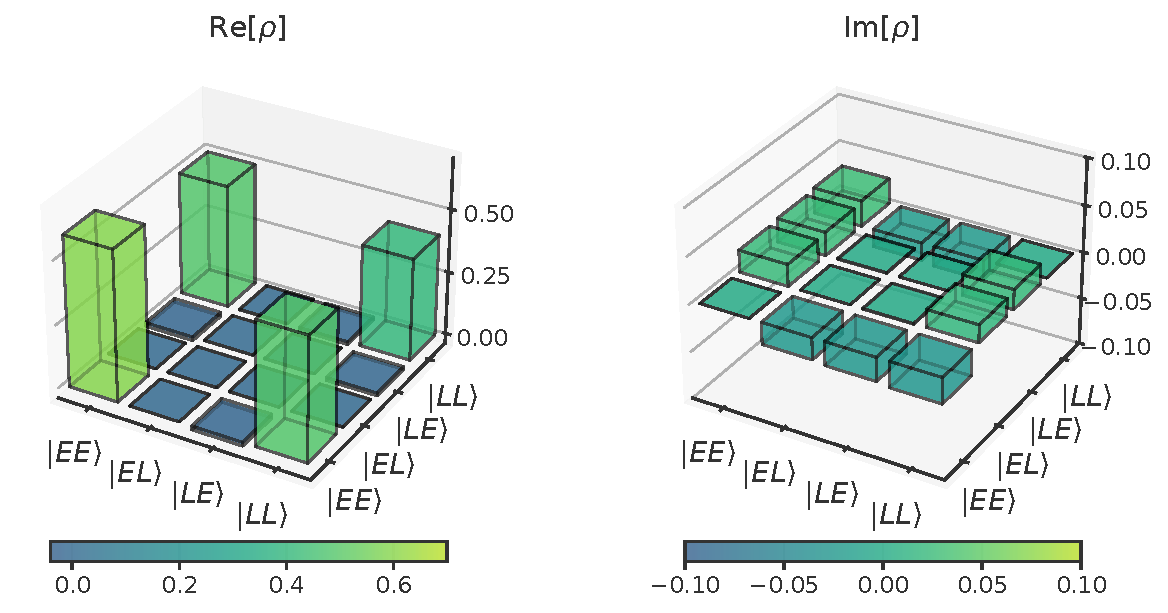
\includegraphics[width=0.9\textwidth,height=\textheight]{./chapter_05/figs/density_matrix_light.pdf}
\caption[{Density matrix at low \(\mu\)}]{\textbf{Density matrix at low $\mu$} Density matrix data from channels 35 and 59 at 1.2 A SHG pump power. The $|ee\rangle$ state is higher than all other states due to the interferometer imbalances. For the matrix shown here, $E_N = 0.971$ and $I_{A\rightarrow B} = 0.904$}
\label{fig:density_matrix}
\end{figure}
}

\hypertarget{impact-of-experimental-imperfections-on-entanglement-visibility}{%
\section{Impact of experimental imperfections on entanglement visibility}\label{impact-of-experimental-imperfections-on-entanglement-visibility}}

\textbf{\emph{Note: the following section is primary written by Samamtha Davis, the second author for the paper on which this chapter is based. It is included here for completeness.}}

The experiment employs three Michaelson interferometers with a path-length delay of 80 ps: one at the source to generate the early and late time-bins, and one prior to each detector to control the measurement basis. To determine the effect of interferometric imperfections on the entanglement visibility, we model the interferometers as equivalent Mach-Zehnder interferometers as shown in Fig.~\ref{fig:interf_model}. Imperfections in the interferometer are captured by the transmittance $t$ of the beamsplitter and internal path (mirror) efficiencies $|\alpha|^2$ and $|\beta|^2$. An ideal Michaelson interferometer has $t = 1/\sqrt{2}$ and $|\alpha|^2 = |\beta|^2 = 1$.

\begin{figure}[h!]
    \centering
    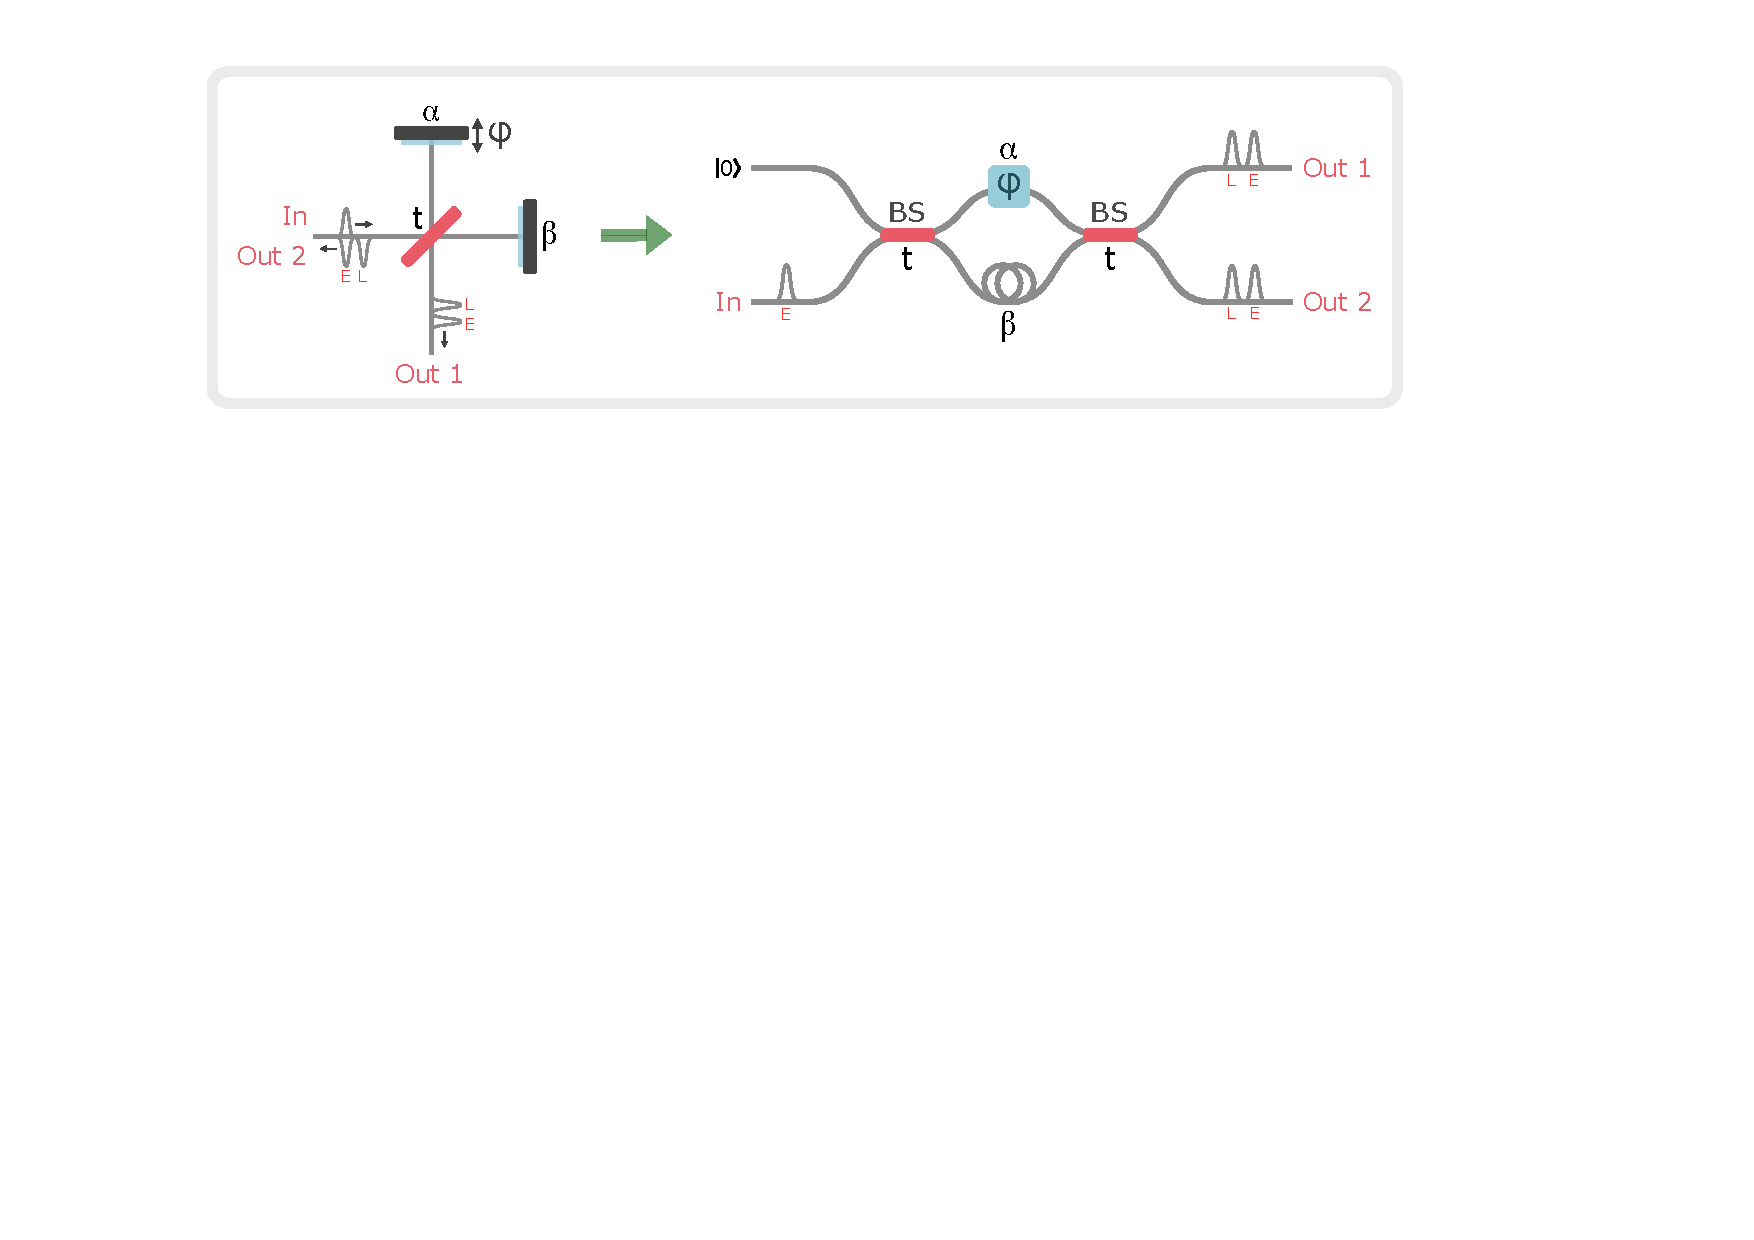
\includegraphics[width=\textwidth]{interf_model.pdf}
    \caption{Model for Michaelson interferometers employed in the experiment. The interfomerter contains a beamsplitter with transmittance $t$ and two mirrors with efficiencies $\alpha$ and $\beta$.}
    \label{fig:interf_model}
\end{figure}

\hypertarget{source-interferometer-imperfections}{%
\subsection{Source Interferometer Imperfections}\label{source-interferometer-imperfections}}

In the experiment, pulses of coherent light from a mode-locked laser (MLL) are injected into the input of the source interferometer. A field $\hat{E}$ at the input of the source interferometer transforms as

\begin{align}
    \hat{E}_{\text{in}}  \rightarrow rt \alpha e^{i\varphi} \hat{E}_{E,1} +  r^2 \alpha e^{i\varphi}\hat{E}_{E,2} + rt\beta \hat{E}_{L,1} + t^2\beta \hat{E}_{L,2} + ir\sqrt{1-|\alpha|^2}\hat{E}_{\text{vac}_1} +it\sqrt{1-|\beta|^2}\hat{E}_{\text{vac}_2} \label{eq:source_field_transform}
\end{align}

where the early and late temporal modes are denoted by subscripts ``E'' and ``L'', the input and output modes are denoted by subscripts ``in'', ``1'' and ``2'', and $r = i\sqrt{1-|t|^2}$. Due to imperfect path efficiencies, part of the light leaks into the vacuum field mode $\hat{E}_{\text{vac}}$, which corresponds to the last term in Eq.~\ref{eq:source_field_transform}. It follows that the power of the early and late output pulses in terms of the power of the input pulse are

\hypertarget{eq:powers}{}{
\begin{align}
    &P_{E,1} = |r|^2|t|^2|\alpha|^2 P_{in},&P_{E,2} = |r|^4 |\alpha|^2 P_{in} \label{eq:powers}\\
    &P_{L,1} = |r|^2|t|^2|\beta|^2 P_{in} ,&P_{L,2} = |t|^4 |\beta|^2 P_{in}.\nonumber 
\end{align}
}

\%The splitting ratio $|t|^2$ and internal path efficiencies $|\alpha|^2$ and $|\beta|^2$ can be solved from ( Eq.~\ref{eq:powers} ).

To generate the entangled photon pairs, one of the output ports of the source interferometer is up-converted by second harmonic generation (SHG) then down-converted via spontaneous parametric down conversion (SPDC), resulting in two-mode squeezed vacuum states (TMSVs) in early and late temporal modes with mean photon numbers $\mu_E$ and $\mu_L$, respectively. The ratio of $\mu_E$ to $\mu_L$ depends on which output port of the source interferometer is used. Note that the definition of $\mu$ used in the main text is per source laser period or per experiment cycle (4.09 GHz). Therefore $\mu$ from the main text is equal to $\mu_E + \mu_L$.
The output power of SHG ($P_{SHG}$) as a function of the SHG pump power ($P_p$) is \autocite{parameswaran2002observation},

\begin{align}
    P_{SHG} = P_{p}\tanh^2{\sqrt{\eta_{SHG}P_{p}}} \approx \eta_{SHG}P_{p}^2
\end{align}

where $\eta_{SHG}$ is the conversion efficiency of the SHG crystal.
After SPDC, the squeezing parameter ($\xi$) of the TMSVs in terms of the SPDC pump power ($P_{SHG}$) is $\xi = \lambda \sqrt{P_{SHG}} \approx \lambda \sqrt{\eta_{SHG}}P_p$, where $\lambda$ is proportional to the SPDC crystal length and nonlinear interaction strength \autocite{kaiser2016fully}.
The mean photon number in terms of the squeezing parameter is $\mu = \sinh^2{\xi}\approx \xi^2$. Therefore, the mean photon numbers of the TMSVs as a function of the output pulses of the source interferometer are,

\begin{align}
    &\mu_E \approx \lambda^2 \eta_{SHG} P_{E,i}^2 &\mu_L\approx \lambda^2 \eta_{SHG} P_{L,i}^2
\end{align}

where $i = 1(2)$ corresponds to output port 1(2) of the source interferometer.

If output port 1 is used, $$\mu_E/\mu_L \approx P_{E,1}^2/P_{L,1}^2 = |\alpha|^4/|\beta|^4,$$ whereas if output port 2 is used, $$\mu_E/\mu_L \approx P_{E,2}^2/P_{L,2}^2 = |r|^8|\alpha|^4/|t|^8|\beta|^4.$$
When output port 1 of the source interferometer is used, if the internal path efficiencies of the source interferometer are different, there is an imbalance in the early and late mean photon numbers. When output port 2 is used, the effect of the imbalance in the internal path efficiencies on the ratio of early and late mean photon numbers can be compensated by imperfect transmittance: $\mu_E/\mu_L = 1$ when $|t|^2/|r|^2 = |\alpha|/|\beta|$.

\hypertarget{measurement-interferometer-imperfections}{%
\subsection{Measurement Interferometer Imperfections}\label{measurement-interferometer-imperfections}}

\begin{figure}[h!]
    \centering
    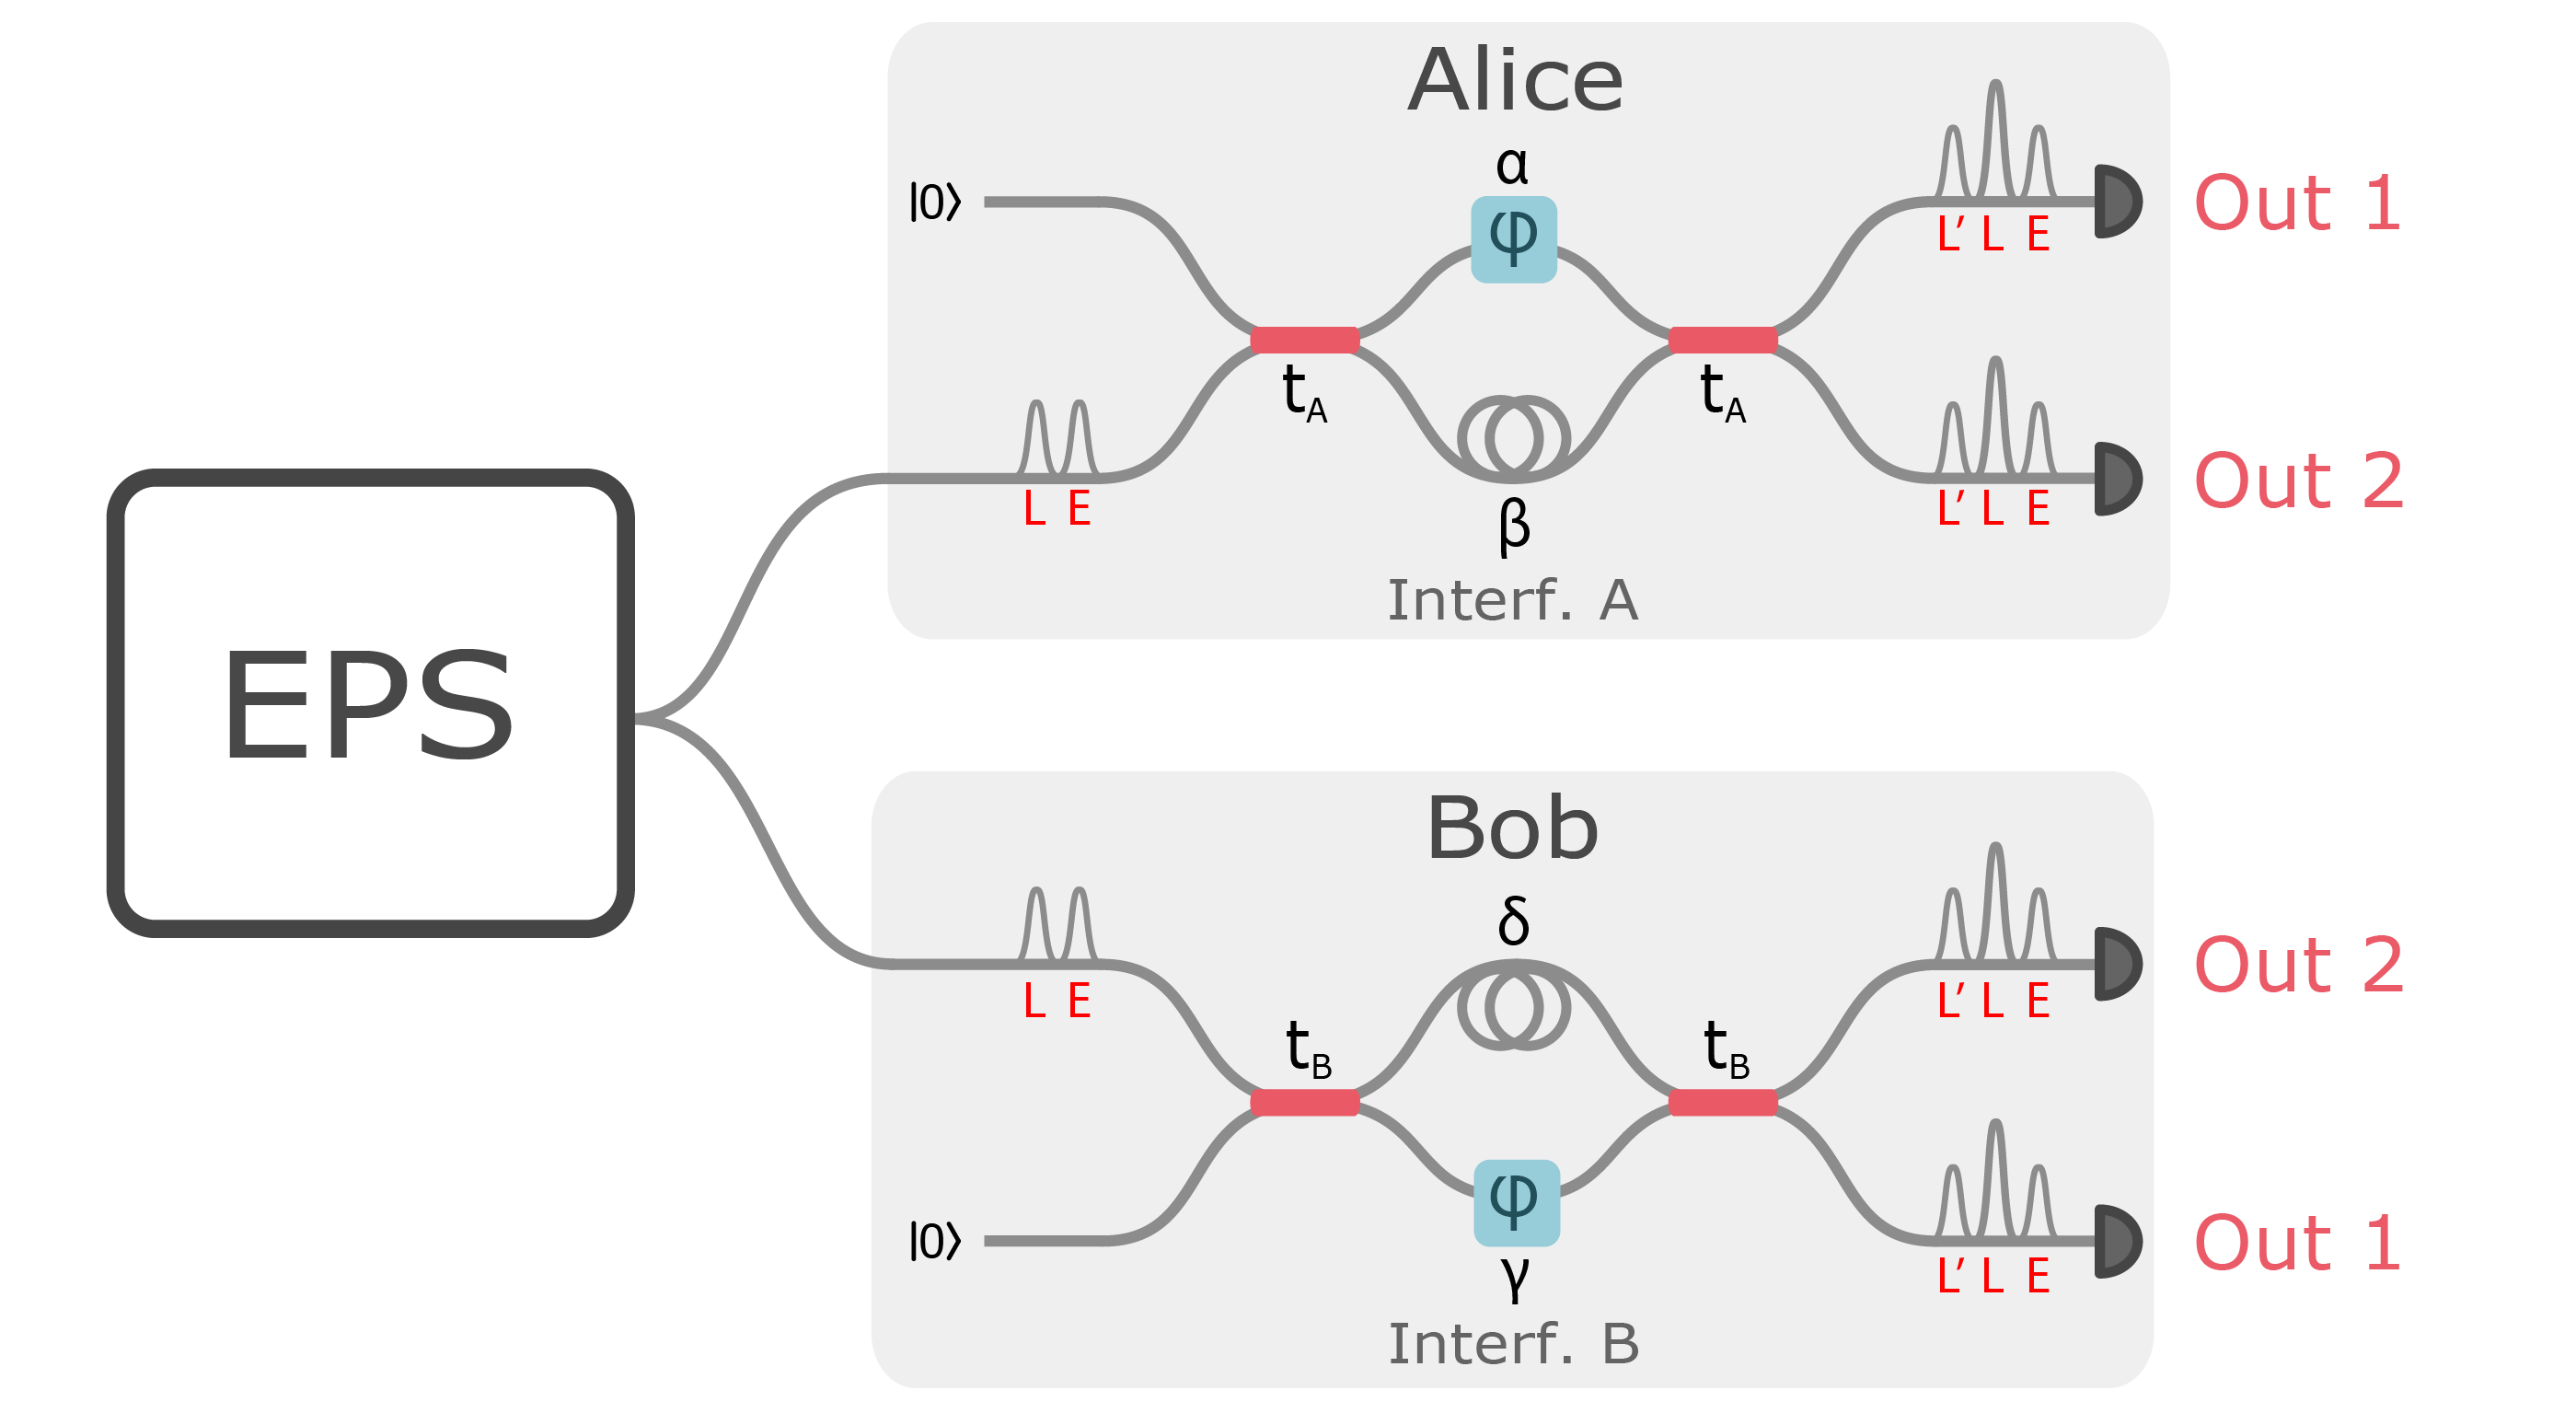
\includegraphics[width=0.8\textwidth]{ent_visib_model.pdf}
    \caption{Setup for theoretical model of entanglement visibility experiment}
    \label{fig:ent_visib_model}
\end{figure}

Imperfections in the measurement interferometers limit the entanglement visibility of the experiment. As described in the previous section, early and late TMSVs are generated by pumping the SPDC with early and late pulses. Each half of each TMSV is sent to a measurement interferometer (see Fig.~\ref{fig:ent_visib_model}). Let $\ket{\xi}$ denote the TMSV state,

\begin{align}
    \ket{\xi} = \sum_{n=0}^{\infty}(-1)^n \sqrt{\frac{\mu^n}{(1+\mu)^{n+1}}}\ket{n_A,n_B}
\end{align}

where $\ket{n_A,n_B}$ denotes the state with $n_A$ photons at the input of interferometer A and $n_B$ photons at the input port of interferometer B. \%As in the previous section, $\mu = \sinh^2{\xi}$ is the mean photon number where $\xi$ is the squeezing parameter.
We model the input state to the measurement interferometers as a product state of TMSV in early and late temporal modes, to lowest order in $\mu_E$ and $\mu_L$:

\hypertarget{eq:input_state}{}{
\begin{align}
    \ket{\Psi_{in}} =& \ket{\xi}_E\otimes \ket{\xi}_L \nonumber \\
    = &\left(\frac{1}{\sqrt{1+\mu_E}}\ket{0,0}_E -\sqrt{\frac{\mu_E}{(1+\mu_E)^2}}\ket{1,1}_E +\cdots\right)
    \otimes \left(\frac{1}{\sqrt{1+\mu_L}}\ket{0,0}_L -\sqrt{\frac{\mu_L}{(1+\mu_L)^2}}\ket{1,1}_L +\cdots\right)\nonumber\\
    \approx& \sqrt{1-(\mu_E +\mu_L)}\ket{0,0}_E \ket{0,0}_L -\sqrt{\mu_E}\ket{1,1}_E  \ket{0,0}_L  -\sqrt{\mu_L}\ket{0,0}_E  \ket{1,1}_L\label{eq:input_state}
\end{align}
}

We can express Eq.~\ref{eq:input_state} in terms of the creation operators $\hat{a}^\dagger$ and $\hat{b}^\dagger$ of the field modes at the inputs of interferometers A and B, respectively:

\hypertarget{eq:input_state_fields}{}{
\begin{align}
    \ket{\Psi_{in}} =\Big(\sqrt{1-(\mu_E+\mu_L)}-\sqrt{\mu_E} \hat{a}_{E}^{\dagger}\hat{b}_{E}^{\dagger} - \sqrt{\mu_L} \hat{a}_{L}^{\dagger}\hat{b}_{L}^{\dagger} \Big)\ket{0,0}_E\ket{0,0}_L \label{eq:input_state_fields}
\end{align}
}

Since the measurement interferometers are also Michaelson interferometers, the transformation relations are,

\hypertarget{eq:aE_transform}{}{
\begin{align}
    &\hat{a}_{E} \mapsto r_At_A \alpha e^{i\varphi} \hat{a}_{E,1} + r_A^2 \alpha e^{i\varphi}\hat{a}_{E,2} + r_At_A\beta \hat{a}_{L,1} + t_A^2\beta \hat{a}_{L,2}+c_A\hat{a}_{\text{vac}_1}+d_A\hat{a}_{\text{vac}_2},\label{eq:aE_transform} 
\end{align}
}

\hypertarget{eq:bE_transform}{}{
\begin{align}
    &\hat{b}_{E}  \mapsto r_Bt_B \gamma e^{i\varphi} \hat{b}_{E,1} + r_B^2 \gamma e^{i\varphi}\hat{b}_{E,2} + r_Bt_B\delta \hat{b}_{L,1} + t_B^2\delta \hat{b}_{L,2}+c_B\hat{b}_{\text{vac}_1}+d_B\hat{b}_{\text{vac}_2},\label{eq:bE_transform}
\end{align}
}

\hypertarget{eq:aL_transform}{}{
\begin{align}
    &\hat{a}_{L} \mapsto  r_A t_A \alpha e^{i\varphi} \hat{a}_{L,1}  + r_A^2 \alpha e^{i\varphi}\hat{a}_{L,2} + r_A t_A\beta \hat{a}_{L^\prime,1}+ t_A^2\beta \hat{a}_{L^\prime,2}+c_A\hat{a}_{\text{vac}_1}+d_A\hat{a}_{\text{vac}_2},\label{eq:aL_transform}
\end{align}
}

\hypertarget{eq:bL_transform}{}{
\begin{align}
    &\hat{b}_{L}  \mapsto r_B t_B \gamma e^{i\varphi} \hat{b}_{L,1} + r_B^2 \gamma e^{i\varphi}\hat{b}_{L,2}  + r_B t_B\delta \hat{b}_{L^\prime,1}+ t_B^2\delta \hat{b}_{L^\prime,2}+c_B\hat{b}_{\text{vac}_1}+d_B\hat{b}_{\text{vac}_2},\label{eq:bL_transform}
\end{align}
}

\begin{align}
    &c_A =ir_A\sqrt{1-|\alpha|^2}, \quad d_A=it_A\sqrt{1-|\beta|^2},\quad
    c_B =ir_B\sqrt{1-|\delta|^2},\quad\ d_B = it_B\sqrt{1-|\gamma|^2},\nonumber
\end{align}

where $L^\prime$ denotes the temporal mode obtained by sending a photon in the late ($L$) mode through the long arm of an interferometer, and $\hat{a}_{\text{vac}_i}$, $\hat{b}_{\text{vac}_i}$ correspond to vacuum modes. To find the state at the output of the interferometers, we combine Eq.~\ref{eq:input_state_fields} with Eq.~\ref{eq:aE_transform} - Eq.~\ref{eq:bL_transform}, and consider only terms relevant to post-selection on coincidences of the middle bins (L) of different interferometer outputs, to lowest order in $\mu_E$, $\mu_L$,

\hypertarget{eq:output_state}{}{
\begin{align}
    \ket{\Psi_{\text{out}}}= %&\sqrt{1-(\mu_E+\mu_L)}\ket{0,0;0,0}_E\ket{0,0;0,0}_L\ket{0,0;0,0}_{L^\prime} \\
    \cdots&+r_A^*t_A r_B^*t_B\Big(\beta \delta\sqrt{\mu_E}+\alpha \gamma \sqrt{\mu_L} e^{-2i\varphi}  \Big)\ket{0,0;0,0}_E\ket{1,0;1,0}_L\ket{0,0;0,0}_{L^\prime}\label{eq: output_state}\\
    &+r_A^*t_A\Big(t_B^2  \beta\delta \sqrt{\mu_E} + (r_B^*)^2  \alpha \gamma \sqrt{\mu_L} e^{-2i\varphi}\Big)\ket{0,0;0,0}_E\ket{1,0;0,1}_L\ket{0,0;0,0}_{L^\prime} \nonumber\\
    &+r_B^*t_B\Big(t_A^2\beta \delta\sqrt{\mu_E}  +(r_A^*)^2 \alpha \gamma  \sqrt{\mu_L} e^{-2i\varphi}\Big)\ket{0,0;0,0}_E\ket{0,1;1,0}_L\ket{0,0;0,0}_{L^\prime} \nonumber\\
    &+\Big(t_A^2 t_B^2\beta \delta\sqrt{\mu_E} + (r_A^*)^2 (r_B^*)^2 \alpha \gamma \sqrt{\mu_L} e^{-2i\varphi}\Big)\ket{0,0;0,0}_E\ket{0,1;0,1}_L\ket{0,0;0,0}_{L^\prime} + \cdots \nonumber 
\end{align}
}

where $\ket{n_{A,1},n_{A_2};n_{B_1}, n_{B,2}}$ denotes the state with $n_{A,1}$ photons at output 1 of interferometer A, $n_{A,2}$ photons at output 2 of interferometer A, $n_{B,1}$ photons at output 1 of interferometer B, and $n_{B,2}$ photons at output 2 of interferometer B. We define the following parameters to simplify notation:

\begin{align}
    x \equiv \frac{\mu_E}{\mu_L},\quad\quad\quad
    \kappa_A \equiv \frac{|\beta|^2}{|\alpha|^2}, \quad\quad\quad \kappa_B \equiv \frac{|\gamma|^2}{|\delta|^2},\quad\quad\quad \epsilon_A = \frac{|t_A|^2}{|r_A|^2}, \quad\quad\quad \epsilon_B \equiv \frac{|t_B|^2}{|r_B|^2}.
\end{align}

From Eq.~\ref{eq:output_state} , it follows that the coincidence probabilities for each combination of output ports are proportional to,

\begin{align}
    &C_{A_1, B_1}(\varphi) \propto \sqrt{\frac{\kappa_B}{\kappa_A}}+\sqrt{\frac{\kappa_A}{\kappa_B}}x+2\sqrt{x}\cos{2\varphi},\\
    &C_{A_1, B_2}(\varphi) \propto \frac{1}{\epsilon_B}\sqrt{\frac{\kappa_B}{\kappa_A}}+\epsilon_B\sqrt{\frac{\kappa_A}{\kappa_B}}x+2\sqrt{x}\cos{2\varphi},\\
    &C_{A_2, B_1}(\varphi) \propto \frac{1}{\epsilon_A}\sqrt{\frac{\kappa_B}{\kappa_A}}+\epsilon_A\sqrt{\frac{\kappa_A}{\kappa_B}}x+2\sqrt{x}\cos{2\varphi},\\
    &C_{A_2, B_2}(\varphi) \propto  \frac{1}{\epsilon_A\epsilon_B}\sqrt{\frac{\kappa_B}{\kappa_A}}+\epsilon_A\epsilon_B\sqrt{\frac{\kappa_A}{\kappa_B}}x+2\sqrt{x}\cos{2\varphi},
\end{align}

where the phase factors in the reflectivities $r_A, r_B$ are absorbed into the definition of $\varphi$. Therefore, the entanglement visibilities, $V = \frac{\text{max}(C(\varphi))-\text{min}(C(\varphi))}{\text{max}(C(\varphi))+\text{min}(C(\varphi))}$, for each combination of output ports are:

\hypertarget{eq:FA1B1}{}{
\begin{align}
    &V_{A_1, B_1} = \frac{2\sqrt{x}}{\sqrt{\frac{\kappa_B}{\kappa_A}}+\sqrt{\frac{\kappa_A}{\kappa_B}}x}, \label{eq:FA1B1}
\end{align}
}

\hypertarget{eq:FA1B2}{}{
\begin{align}
    &V_{A_1, B_2} = \frac{2\sqrt{x}}{\frac{1}{\epsilon_B}\sqrt{\frac{\kappa_B}{\kappa_A}}+\epsilon_B\sqrt{\frac{\kappa_A}{\kappa_B}}x},\label{eq:FA1B2}
\end{align}
}

\hypertarget{eq:FA2B1}{}{
\begin{align}
    &V_{A_2, B_1} =  \frac{2\sqrt{x}}{ \frac{1}{\epsilon_A}\sqrt{\frac{\kappa_B}{\kappa_A}}+\epsilon_A\sqrt{\frac{\kappa_A}{\kappa_B}}x},\label{eq:FA2B1}
\end{align}
}

\hypertarget{eq:FA2B2}{}{
\begin{align}
    &V_{A_2, B_2} = \frac{2\sqrt{x}}{\frac{1}{\epsilon_A\epsilon_B}\sqrt{\frac{\kappa_B}{\kappa_A}}+\epsilon_A\epsilon_B\sqrt{\frac{\kappa_A}{\kappa_B}}x}.\label{eq:FA2B2}
\end{align}
}

Unity visibility is achievable for each combination of output ports: $V_{A_1, B_1} = 1$ when $x = \kappa_B/\kappa_A$, $V_{A_1, B_2} = 1$ when $x = \kappa_B/(\kappa_A\epsilon_B^2)$, $V_{A_2, B_1} = 1$ when $x = \kappa_B/(\kappa_A\epsilon_A^2)$, and $V_{A_2, B_2} = 1$ when $x = \kappa_B/(\kappa_A\epsilon_A^2\epsilon_B^2)$. Therefore, the effect of imbalances in the source and measurement interferometers is to shift the optimal ratio of early to late mean photon numbers. Imbalances in the measurement interferometers can be compensated by imbalances in the source interferometer in order to obtain unity visibility. Moreover, in the single photon limit, the visibility is insensitive to the absolute path efficiencies in the experiment. The visibility depends only on the ratio of path efficiencies between the measurement interferometers ( $\kappa_A/\kappa_B$ ). The entanglement visibilities for each combination of output ports as a function of $x=\mu_E/\mu_L$ for various ratios of interferometric path efficiencies are shown in Fig.~\ref{fig:ent_fid_single_photon}.

\begin{figure}[H]
    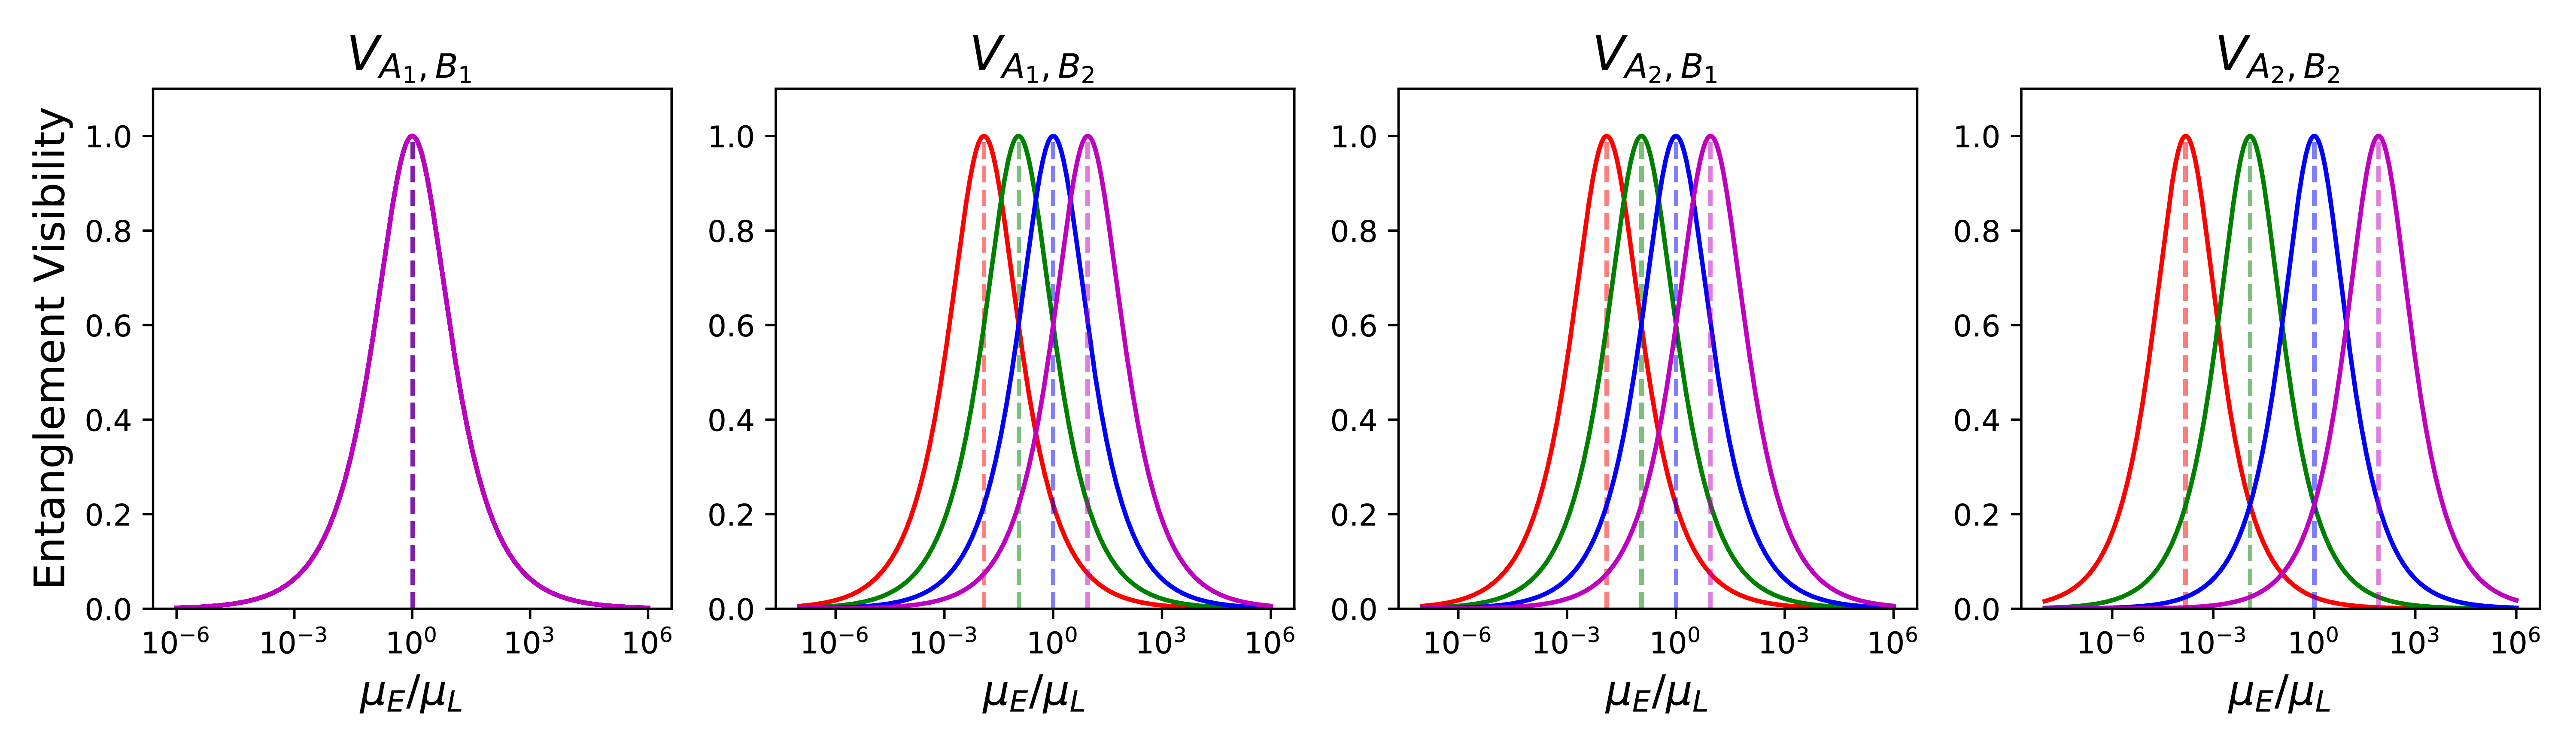
\includegraphics[width = \textwidth]{ent_fid_single_photon_fixed_kappa.pdf}
    \caption{Entanglement visibility as function of $\mu_E/\mu_L$ for fixed $\kappa_B/\kappa_A = 1$ and  $ \epsilon_A = \epsilon_B = 90/10$ (red), $75/25$ (blue), $50/50$ (green), $25/75$ (purple).}
    \label{fig:ent_fid_single_photon}
\end{figure}

\hypertarget{multiphoton-effects}{%
\subsection{Multiphoton Effects}\label{multiphoton-effects}}

\begin{figure}[h!]
    \centering
    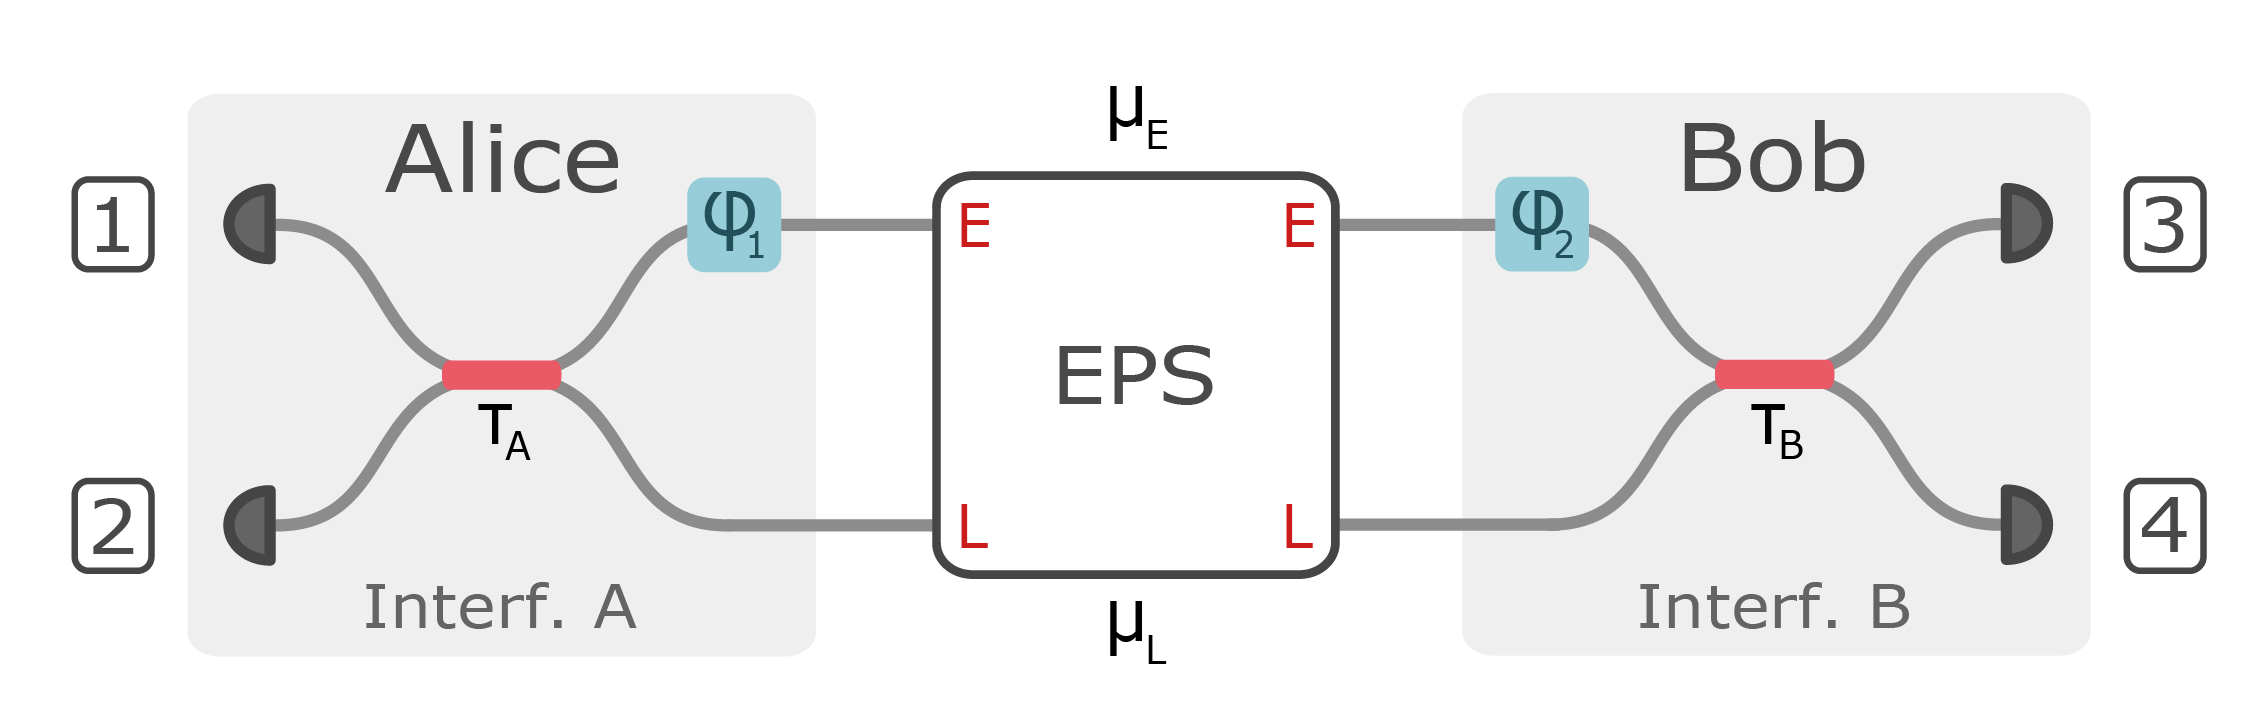
\includegraphics[width = \textwidth]{model_setup.pdf}
    \caption{Setup for phase space modeling of entanglement visibility experiment}
    \label{fig:model_setup}
\end{figure}

Calculating the entanglement visibility to higher order photon number contributions quickly becomes intractable with the Fock space approach in section B. To study the effect of multiphoton events on the entanglement visibility, we model the experiment using phase space methods based on a characteristic function formalism \autocite{Davis2022,takeoka2015full}. The model setup is shown in Fig.~\ref{fig:model_setup}. As in the Fock space approach, the input state is modeled as a product state of TMSV in early and late temporal modes, with mean photon numbers $\mu_E$ and $\mu_L$, respectively. The measurement interferometers are modeled as beamsplitters in the temporal domain that mix the early and late input modes with transmittances $\tau_A$ and $\tau_B$, which absorb the interferometric path efficiencies and spatial beamsplitter transmittances. Since the input state is modeled as a Gaussian state, and the measurement interferometers are modeled as Gaussian operations, we can find the symplectic transformation that maps the characteristic function of the input state to that of the state prior to detection.

Following Ref. \autocite{Davis2022}, the characteristic function for an $N$-mode bosonic state is

\begin{align}
    \chi(\xi)=\text{Tr}\left[\hat{\rho}\exp(-i(\hat{x}_1,\hat{p}_1,\hat{x}_2,\hat{p}_2,\cdots\hat{x}_N,\hat{p}_N) \xi)\right]
\end{align}

where $\xi\in \mathbb{R}^{2N}$, $\rho$ is the density matrix, and $\hat{x}_i = \frac{1}{\sqrt{2}}(\hat{a}_i^\dagger+\hat{a}_i)$ and $\hat{p}_i=\frac{1}{\sqrt{2}}(\hat{a}_i^\dagger+\hat{a}_i)$ are the quadrature operators for mode $i$ with annihilation operator $\hat{a}_i$.
A Gaussian state is a state whose characteristic function that takes a Gaussian form,

\begin{align}
    \chi(\xi) = \exp(-\frac{1}{4}\xi^T\gamma \xi - id^T \xi),
\end{align}

which is fully characterized by the displacement vector $d$ and covariance matrix $\gamma$, i.e.~the first and second moments.
For the TMSV state, the displacement vector is the null vector $d =(0,0,0,0)$ and the covariance matrix is given by

\begin{align}
    \gamma_{TMSV}(\mu) = 
    \begin{pmatrix}
    \mathbf{A}&\mathbf{B}\\
    \mathbf{B}&\mathbf{A}
    \end{pmatrix}, \quad
    \mathbf{A}=
    \begin{pmatrix}
        1+2\mu&0\\
        0&1+2\mu
    \end{pmatrix}, \quad
    \mathbf{B}=\begin{pmatrix}
        2\sqrt{\mu(\mu+1)}&0\\
        0&-2\sqrt{\mu(\mu+1)}
    \end{pmatrix}
\end{align}

where $\gamma_{TMSV}(\mu)$ is written in block matrix form. Therefore, the covariance matrix for the input state of our experiment is

\begin{align}
    \gamma_{in}(\mu_E,\mu_L) = \gamma_{TMSV}(\mu_E)\oplus \gamma_{TMSV}(\mu_L)
\end{align}

The characteristic function of the input state is mapped to the characteristic function of the state prior to detection by a symplectic transformation,

\begin{align}
    \chi_{in}(\xi) = \exp(-\frac{1}{4}\xi^T\gamma_{in} \xi)\mapsto \chi_{out}(\xi) = \exp(-\frac{1}{4}\xi^T S^T \gamma_{in}S \xi)
\end{align}

where $S$ is the Symplectic matrix of the interferometers. We construct $S$ from the Symplectic matrices of the phase shifter ($S_{PS}$) and beamsplitter ($S_{BS}$) \autocite{takeoka2015full},

\begin{align}
    &S_{PS}(\varphi) = \begin{pmatrix}
        \cos{\varphi}&\sin{\varphi}\\
        -\sin{\varphi}&\cos{\varphi}
    \end{pmatrix},\\
    &S_{BS}(\tau) = 
    \begin{pmatrix}
    \mathbf{T}&\mathbf{R}\\
    \mathbf{R}&\mathbf{T}
    \end{pmatrix}, \quad
    \mathbf{T}=\begin{pmatrix}
        \tau&0\\
        0&\tau
    \end{pmatrix}, \quad \mathbf{R}=
    \begin{pmatrix}
    0&-\sqrt{1-\tau^2}\\
    \sqrt{1-\tau^2}&0
    \end{pmatrix}.
\end{align}

From the output characteristic function $\chi_{\text{out}}$, we obtain the coincidence probabilities using Eq. (9) of Ref. \autocite{Davis2022},

\begin{align}
    \text{Tr}\left[\hat{\rho}_{\text{out}}\hat{\Pi}\right] = \left(\frac{1}{2\pi}\right)^N \int {dx}^{2N}\chi_{\text{out}} (x) \chi_\Pi (-x)
\end{align}

where $\hat{\rho}_{\text{out}}$ is the state prior to detection with characteristic function $\chi_{\text{out}}$, and $\hat{\Pi}$ is the measurement operator corresponding to coincidences between detectors from different interferometers. The measurement operators for a threshold detector, which distinguishes between a detection event (at least one photon) and no detection event (zero photons), are

\begin{align}
    \hat{\Pi}_{\text{event}} = \hat{I}-\ket{0}\bra{0}, \quad  \hat{\Pi}_{\text{no event}} = \ket{0}\bra{0}
\end{align}

where $\hat{I}$ is the 2 by 2 identity matrix.
The measurement operator for coincidences between e.g.~detectors 1 and 4 are

\begin{align}
    \hat{\Pi}_{1,4}=\hat{\Pi}_{\text{event},1}\otimes\hat{I}_2 \otimes \hat{I}_3 \otimes \hat{\Pi}_{\text{event},4}
\end{align}

where the subscripts denote the output modes labeled in Fig.~\ref{fig:model_setup}. We derive an analytical expression for the coincidence probability that encompasses all multiphoton contributions,

\begin{align}
C(\varphi) =  \text{Tr}\left[\hat{\rho}_{\text{out}}\hat{\Pi}_{1,4}\right] &= 1-\frac{1}{|f(\mu_E, \mu_L, \tau_A)|}-\frac{1}{|g(\mu_E, \mu_L, \tau_B)|}+\frac{1}{|h(\mu_E, \mu_L, \tau_A, \tau_B,\varphi)|},\\
f(\mu_E, \mu_L, \tau_A) &= 1+\mu_L+\tau_A(\mu_E - \mu_L),\\
g(\mu_E, \mu_L, \tau_B) &= 1+\mu_E+\tau_B(\mu_L - \mu_E),\\
h(\mu_E, \mu_L, \tau_A, \tau_B) &=1+\mu_E + \mu_L(1 + \mu_E)(1 -\tau_A) \\
&-\mu_E\tau_B(1 + \mu_L) +\tau_A\tau_B(\mu_E  + \mu_L +2\mu_E\mu_L) \nonumber\\
&- 2\sqrt{\mu_E\mu_L\tau_A(1+\mu_E)(1+\mu_L)(1-\tau_A)}\sqrt{\tau_B(1-\tau_B)}\cos{\varphi},\nonumber
\end{align}

where $\varphi = \varphi_A-\varphi_B$ is the relative phase between interferometers A and B.
The different visibilities in each output port combination as a result of interferometric imbalances can be obtained by adjusting $\tau$ accordingly. To isolate the impact of multiphoton contributions to the visibility, we set $\tau_A = \tau_B = \frac{1}{\sqrt{2}}$, and obtain the following expression for the entanglement visibility:

\hypertarget{eq:fid_multiphoton}{}{
\begin{align}
    V(\mu_E, \mu_L) &= \frac{C(0)-C(\pi)}{C(0)+C(\pi)}=\frac{2/\sqrt{G_{-}(\mu_E, \mu_L)}-2/\sqrt{G_{+}(\mu_E, \mu_L)}}{1-4/(2+\mu_E+\mu_L)+2/\sqrt{G_{-}(\mu_E, \mu_L)}+2/\sqrt{G_{+}(\mu_E, \mu_L)}}\label{eq:fid_multiphoton}
\end{align}
}

where

\begin{align}
     G_{\pm}(\mu_E, \mu_L)&=\mu_E^2(9+8\mu_L(2+\mu_L))\\
     &\pm(4+3\mu_L)\bigg(\pm4\pm3\mu_L+4\sqrt{\mu_E \mu_L (1+\mu_E)(1+\mu_L)}\bigg)\nonumber\\     &+2\mu_E\bigg(12\pm6\sqrt{\mu_E\mu_L(1+\mu_E)(1+\mu_L)}\bigg)\nonumber\\
     &+2\mu_E\mu_L\Big(19+8\mu_L \pm 4\sqrt{\mu_E\mu_L (1+\mu_E)(1+\mu_L)}\Big). \nonumber
 \end{align}

By expanding Eq.~\ref{eq:fid_multiphoton} to first order in $\mu_E$ and $\mu_L$,

\hypertarget{eq:fid_first_order}{}{
\begin{align}
    V(\mu_E,\mu_L) = \frac{2\sqrt{\frac{\mu_E}{\mu_L}}}{1+\frac{\mu_E}{\mu_L}} - \frac{\mu_E}{\mu_L}\frac{\left(5(\frac{\mu_E}{\mu_L}+\frac{\mu_L}{\mu_E})+6\right)}{2(1+\frac{\mu_E}{\mu_L})^2}\sqrt{\mu_E\mu_L}+\cdots\label{eq: fid_first_order}
\end{align}
}

we see that the first term matches Eq.~\ref{eq:FA1B1} - Eq.~\ref{eq:FA2B2} for $t_A = t_B = \frac{1}{\sqrt{2}}$, $\beta/\alpha = \gamma/\delta = 1$. Moreover, for $\mu_{eq} \equiv \mu_E = \mu_L$, Eq.~\ref{eq:fid_first_order} reduces to $V(\mu_{eq}) = 1 - 2\mu_{eq}$.

Thus, the upper bound on the visibility is set by the mean photon number, i.e.~multiphoton effects. Entanglement visibilities of more than 90\% are possible when $0.39 < \mu_E/\mu_L < 2.55$ and $\mu_L < 0.0.056$. The entanglement visibility $V(\mu_E, \mu_L)$ in Eq.~\ref{eq:fid_multiphoton} is plotted for various mean photon numbers in Fig.~\ref{fig:fid_multiphoton}.

\begin{figure}[H]
\centering
    \begin{subfigure}{0.75\textwidth}
        \centering
        \includegraphics[width = \textwidth]{Fid_vs_mu_above_1.pdf}
    \end{subfigure}
    \bigskip
    \begin{subfigure}{0.75\textwidth}
        \centering
        \includegraphics[width = \textwidth]{Fid_vs_mu_below_1.pdf}
    \end{subfigure}
    \caption{Entanglement visibility as a function of mean photon number for $\tau_A = \tau_B = 1/\sqrt{2}$.}
    \label{fig:fid_multiphoton}
\end{figure}

\hypertarget{time-walk-correction}{%
\section{Time-Walk Correction}\label{time-walk-correction}}

SNSPD jitter increases with count rate due to properties of the nanowire reset process and features of the readout circuit. A threshold timing measurement set at a specific trigger level will `walk' along the rising edge of SNSPD pulses by varying amounts if those pulses vary in amplitude and slew rate. At low count rates, SNSPDs exhibit very uniform pulse heights and shapes. However, at high counts rates where the inter-arrival time is on the order of the reset time of the detector, current-reset and amplifier effects lead to smaller and distorted pulses in a form of pulse `pile-up'~\cite{Mueller2023}.

\begin{figure}[H]
    \centering
    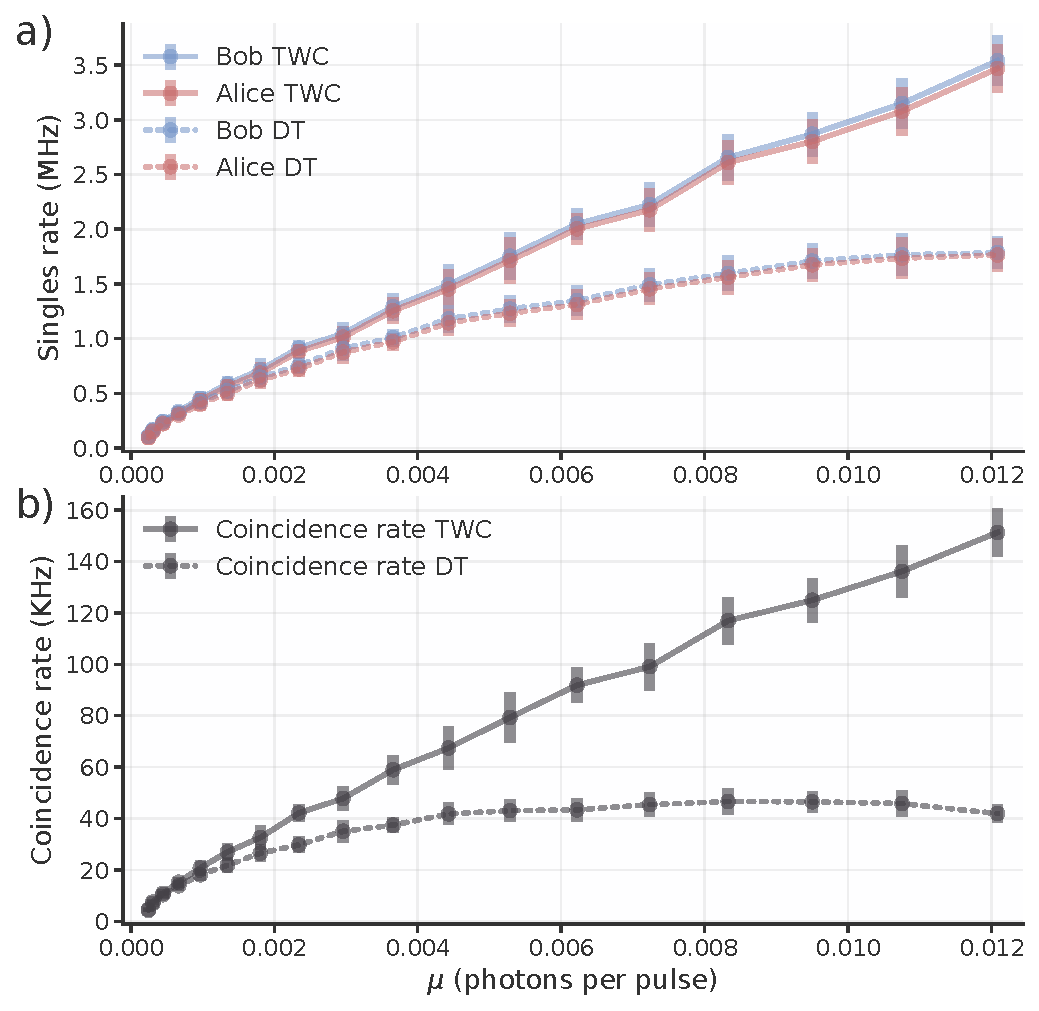
\includegraphics[width=0.7\linewidth]{time_walk_comparison_light.pdf}
    \caption{a) Adding 200~ns dead time (DT) to avoid high-rate jitter significantly reduces count rates at higher $\mu$. With time walk correction (TWC), the full available count rate is preseved while keeping the timing jitter low. b) The reduction in count rate for coincidences is more dramatic, because the lost efficiency at both detectors contrinbutes. }
    \label{fig:time_walk_vs_dead_time}
\end{figure}

The effects of time walk can be filtered out by imposing a dead time following each detection. The length of the dead time is tuned so that SNSPD events arriving within it are expected to have distorted timing, and are thrown out. However, as shown in \ref{fig:time_walk_vs_dead_time}, this method can severely limit count and coincidence rates for detector types that exhibit long periods of undershoot or ringing on the falling edge of the RF pulse. For the differential SNSPDs used here, a 200~ns dead time would be necessary to filter out all time-walk effects.

As detailed in \cite{Mueller2023, Craiciu23}, a calibration and correction process may be used to cancel out the effects of time walk without losing count rate. It relies on adding timing corrections $\tilde{d}$ to time-distorted SNSPD time tags based on the inter-arrival $t'$ time that precedes each tag. Building a lookup table for $\tilde{d}$ as a function of $t'$ is the objective of the calibration process. With this, real-time running software may largely cancel the increase in jitter from time-walk.

Here we introduce a simplification of the calibration process from \cite{Mueller2023} that makes use of the pulse sequence already impinging on the detectors from the entanglement source. With the calibration routine written directly into our coincidence analysis software, recomputing the ideal $t'-vs-\tilde{d}$ curve takes no more than a few seconds whenever the detector bias currents or trigger levels are changed.

We have previously shown how the $t'-vs-\tilde{d}$ curve can be found by illuminating the detector with photons from a pulsed laser source \cite{Mueller2023}. We imposed the requirement that the period $p$ of the pulses sequence be larger that the largest expected jitter observed due to time walk. This way, any time-tag can be unambiguously associated with the timing of the laser pulse that created it, thereby inferring the relation between $t'$ and $\tilde{d}$ for that event.

Here we rely on a 2D histogram that plots $t'$ on the y-axis and the usual clock-referenced arrival time on the x-axis. Here, any single $t'$ and absolute arrival time measurement does not imply a correction $\tilde{d}$ when considered in isolation. This is because the time-distribution is an irregular pattern of histogram peaks of varying height, as opposed to a more uniform sequence. Also, delays $\tilde{d}$ can surpass the experiment's fundamental period (244.5~ps from the laser's 4.09~GHz rep rate), initially complicating the matching of trigger events to originating photon timing. But despite these nuances, the 2D histogram structure implies a method for extracting the $t'-vs-\tilde{d}$ calibration curve through a special analysis.

Slices at the bottom of the 2D histogram (fig.~\ref{fig:time_walk}a) for large $t'$ are essentially identical to the low-count-rate 3-peak singles histograms like from figure 2c in the main text. As $t'$ decreases from here, the slice as a whole develops some linear offset or rollover (periodic every 244.5~ps). This offset is the $\tilde{d}$ offset of interest. Therefore, $t'-vs-\tilde{d}$ may be extracted by running a template matching algorithm on each horizontal slice, using the large-$t'$ slice as the template. We opt for a absolute differences algorithm (fig.~\ref{fig:time_walk}b). As the algorithm progress to smaller and smaller $t'$, the offset may approach the fundamental period length and `roll over' causing a jump-discontinuity. But this can be detected and corrected for, meaning the method may produce a $t'-vs-\tilde{d}$ curve (fig.~\ref{fig:time_walk}c) with some $\tilde{d}$ larger than the fundamental period.

\begin{figure}[H]
    \centering
    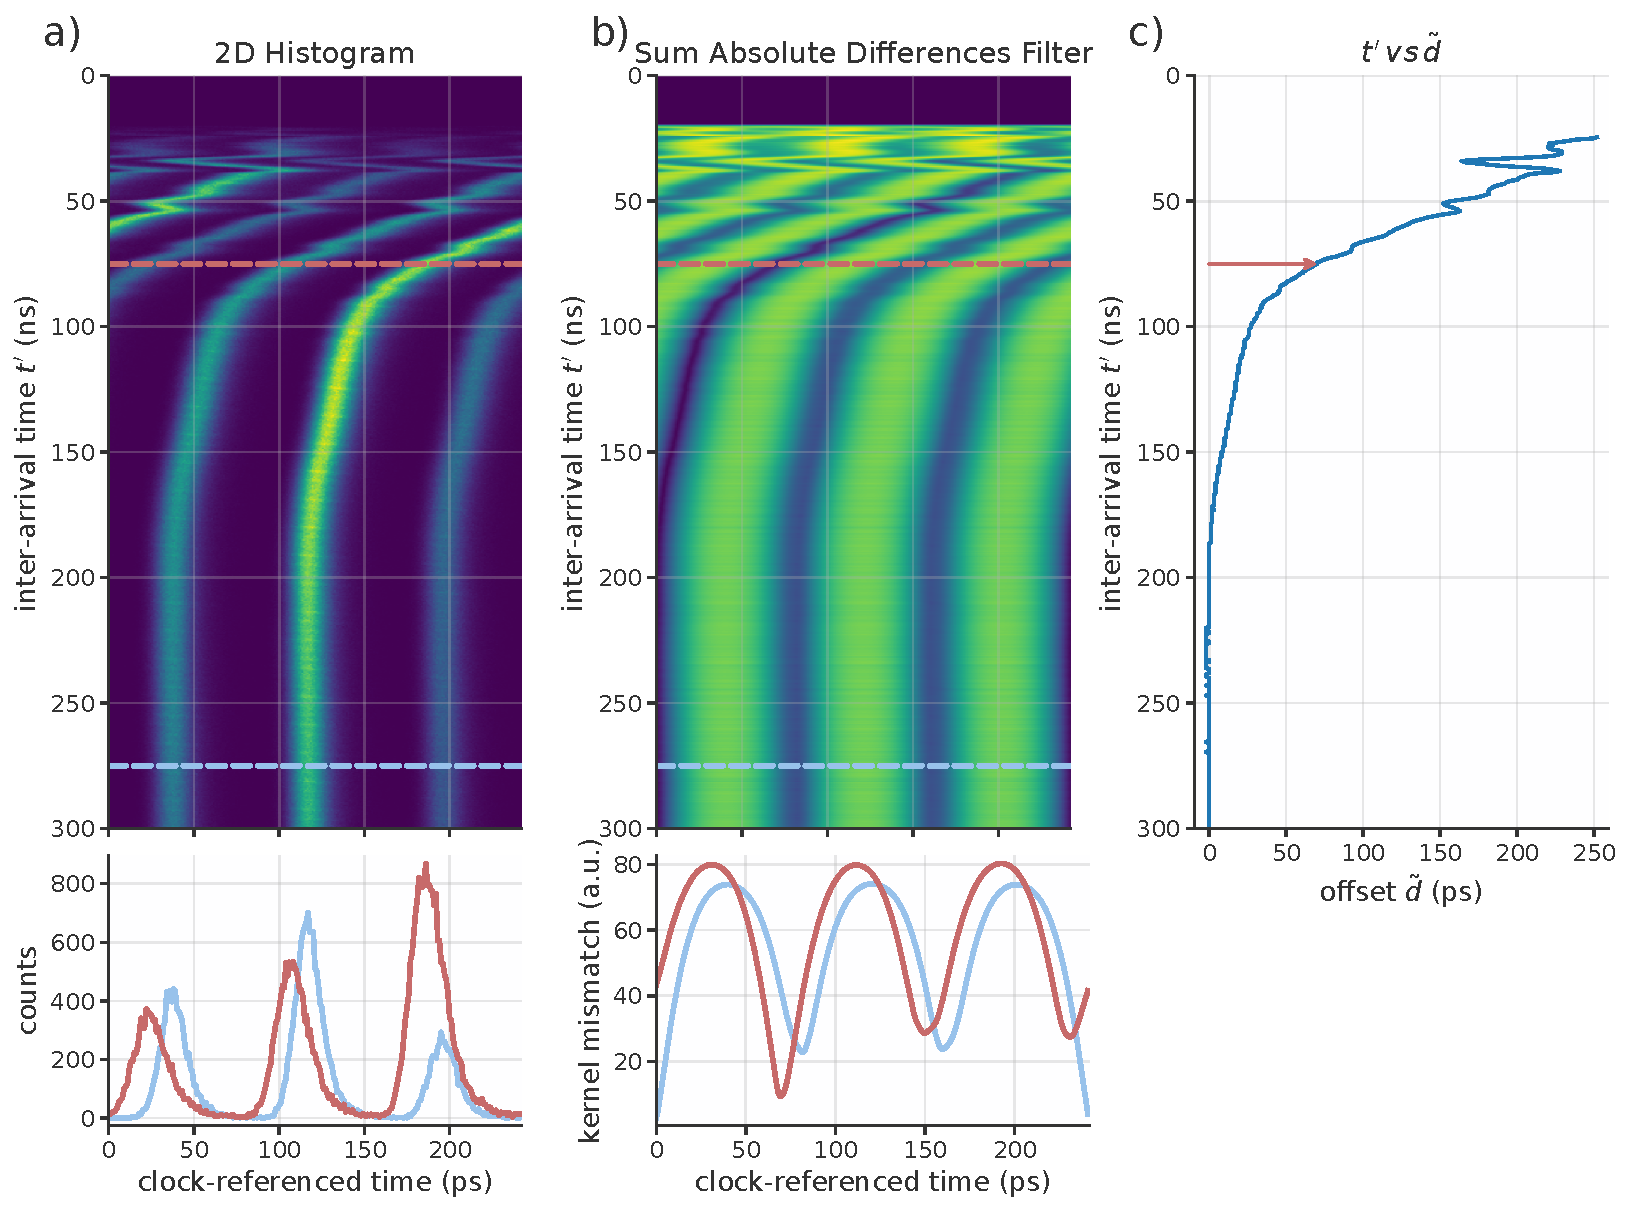
\includegraphics[width=0.8\linewidth]{time_walk_analysis.pdf}
    \caption{a) The 2d histogram with clock-referenced histograms on the x-axis and inter-pulse arrival time $t'$ on the y-axis. The effect of time walk is evident in the horizontal translations of the 3-peak structure as $t'$ decreases. Slices of the 2D histogram indicated by the red and blue horizontal line are plotted as regular histograms in the lower figure. b) After applying the Sum Absolute Differences filter to horizontal slices of the 2D histogram. The $t'-vs-\tilde{d}$ delay curve (c) is extracted from this by using the index of each row with minimum mismatch value as the $\tilde{d}$ value for that row.}
    \label{fig:time_walk}
\end{figure}

Overall, time-walk analysis based on the 2D histogram construction is straightforward to implement and user friendly because it may be applied \textit{in situ} as part of software that already creates histograms and records coincidences.

\hypertarget{filter-bandwidths}{%
\section{Filter Bandwidths}\label{filter-bandwidths}}

\begin{figure}[H]
    \centering
    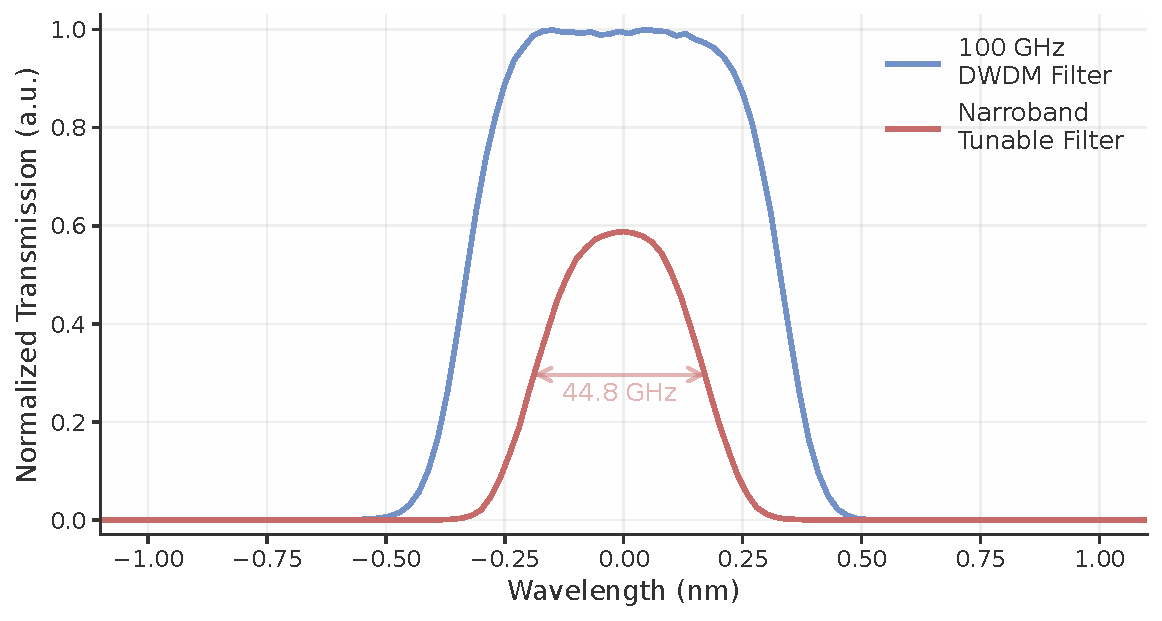
\includegraphics[width=0.7\linewidth]{filter_comparison_light.pdf}
    \caption{Spectrums for a single DWDM channel and narroband filter, with the center wavelengths set to zero. The narroband filter is used at Bob with the 16-channel DWDM at Alice to measure coincidence rates in the main text Fig. 2b. For the 100~GHz spec. DWDM filters, 100~GHz refers to the filter spacing. The FWHM passband for each is about 82~GHz.}
\end{figure}

\hypertarget{guard-regions}{%
\section{Guard Regions}\label{guard-regions}}

The width $x$ of the guard regions centered at 80 and 160 ps were set to 10~ps. As shown in Fig. \ref{fig:guard_scan}, this width increase fidelities slightly without significantly impacting coincidence rates. 10~ps was not chosen based on rigorous analysis, though it would be possible to optimize the width to maximize some metric, like secret key rate.

\begin{figure}[h]
    \centering
    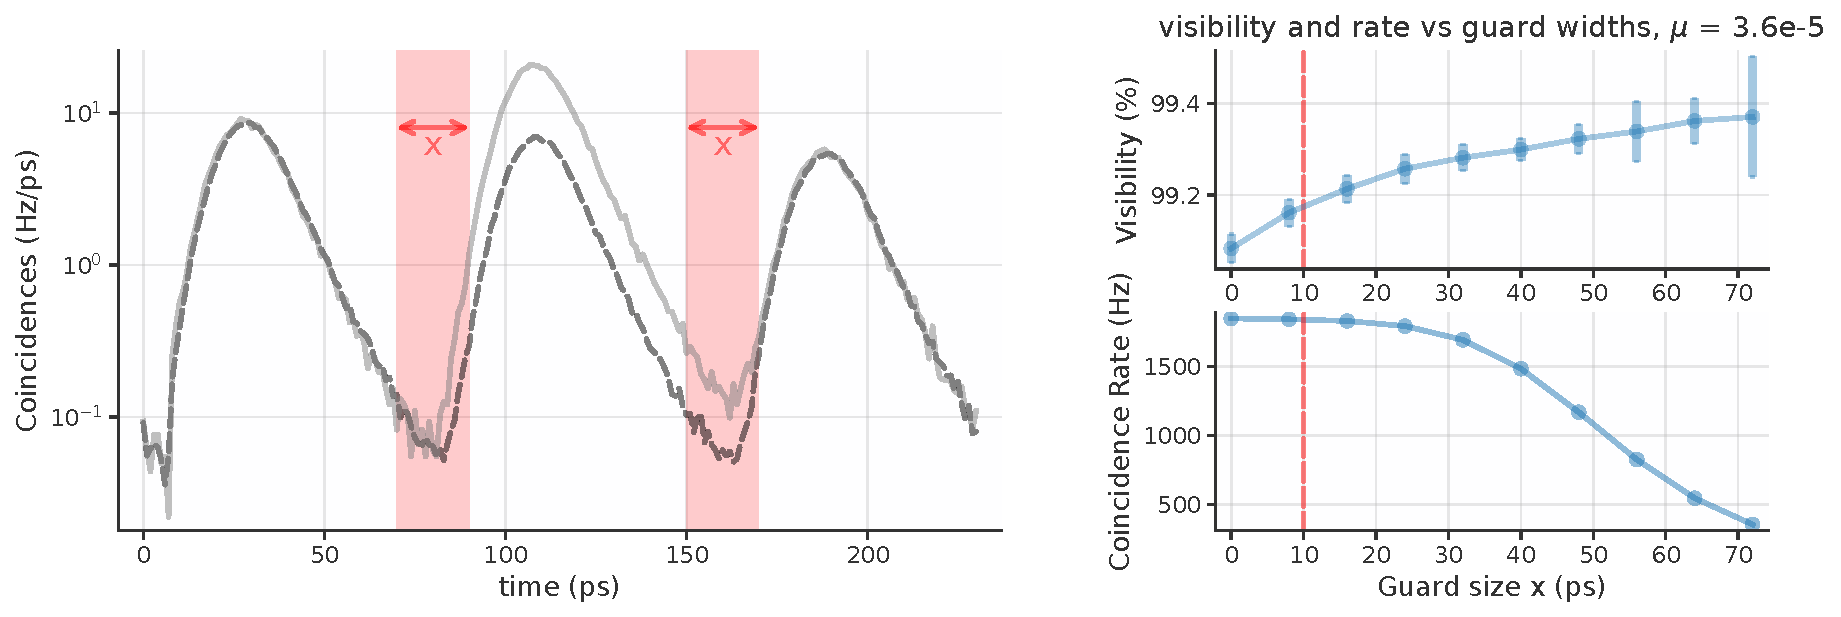
\includegraphics[width=1\linewidth]{guard_scan_light.pdf}
    \caption{Charts on the right show phase basis fidelities and total coincidence rates as a function of width $x$, where both guard regions stay centered at 80 \& 160~ps.}
    \label{fig:guard_scan}
\end{figure}

\hypertarget{incompatible-bases-accidental-coincidence-rate}{%
\section{Incompatible Bases \& Accidental Coincidence Rate}\label{incompatible-bases-accidental-coincidence-rate}}

An entangled pair can be called `spectrally compatible' with a given DWDM channel pairing if --given no losses-- it would be detected 100\% of the time across that channel pair. In the case where signal and idler modes are perfectly spectrally compatible, it has been shown that accidental coincidences still negatively impact visibilities \cite{Kim2022}. In this case and assuming negligible dark counts, visibility is reduced as:

$$
\begin{aligned}
V = \frac{1}{1+\mu}V_0
\end{aligned}
$$

Where $V_0$ is a nominal interferometer-limited visibility \cite{Kim2022} and $\mu$ is the mean photon number per pulse (classically defined like with \ref{eq:colorless}). The accidental coincidence rate discussed in the main text $C_{Acc}$ is only partially related to this, as it specifically takes into account only accidental coincidences due to incompatible spectral modes. Such coincidences can arise from two situations, and can be assigned their own coincidence rates

\begin{itemize}
\item $C_{ee}$: two photons both from mutually incompatible spectral regions, like the red regions in Fig. \ref{fig:narroband}c 
\item $C_{em}$ and $C_{me}$: one photon from the central overlapping filter region and one from an incompatible spectral region. 
\end{itemize}

Say one member of a spectrally compatible entanglemed pair reaches Alice, but not Bob due to loss. The photon received at Alice could form a coincidence with a spectrally incompatible photon that arrives at Bob. These are the $C_{em}$ and $C_{me}$ type coincidences. $C_{Acc}$ in the main text is the sum of $C_{ee}$, $C_{em}$ and $C_{me}$:

\begin{align}
    C_{Acc} &= C_{ee} + C_{em} + C_{me} \\
    C_{ee}/R &= (1 - \delta)\frac{S_A}{R} * (1 - \delta)\frac{S_B}{R} \\
    C_{em}/R &= (1 - \delta)\frac{S_A}{R} * \delta (1-\eta_A) \frac{S_B}{R} \\
    C_{me}/R &= (1 - \delta)\frac{S_B}{R} * \delta (1-\eta_B) \frac{S_A}{R} \\
\end{align}
\begin{align}
C_{Acc} = \frac{1}{R}(1 - \delta) S_A S_B \left(\delta \left(1-\eta _A\right)+\delta \left(1-\eta _B\right)+1-\delta\right)
\end{align}

\hypertarget{maximum-entangled-photon-source-throughput}{%
\section{Maximum Entangled Photon Source Throughput}\label{maximum-entangled-photon-source-throughput}}

We observe in the small $\mu$ limit that the metrics $V$, $E_N = C_N/C_{AB}$, $E_I = C_I/C_{AB}$, and $E_S = SKR/C_{AB}$ scale linearly with $\mu$, where $E_S$ is the secret key fraction. Raw coincidence rate is not linear with $\mu$ due to the count rate dependent efficiency of the SNSPDs. As count rate increases, the detector spends a larger fraction of time in a partially reset state where photo-detection is less efficient or not possible. We separately collect measurements of detector efficiency versus count rate extending past 10~Mcps, and use this to extrapolate coincidence rate to higher powers. Then, the metrics $E_N$, $E_I$, and $E_S$ are multiplied by the extrapolated rate to define extrapolated $C_N$, $C_I$, and $SKR$ as shown in \ref{fig:scan_extrapolate}b. Maximum values of these metrics are highlighted by colored circular markers.

In this work we primarily study the capability of 8 DWDM channel pairs, with some analysis of 16-pair performance. However, the spectrum of entangled photon pairs produced by the type-0 SPDC is quite broad, meaning spectral multiplexing across many more channels is possible. In \ref{fig:scan_extrapolate} the spectrum of the SPDC is overlayed with sixty 100~GHz DWDM channel pairs spanning the L, C, and S ITU bands {[}L-29 (1592.1~nm) through C-20 (1543.73) and C-10 (1535.82) through S-1 (1490.76){]}. The coincidence rate through these added channels can be estimated from this spectrum and the known performance of the central 8 channel pairs. Table 1 in the main text specifies estimates for the total rate from the 60 multiplexed spectral channels.

\begin{figure}[H]
    \centering
    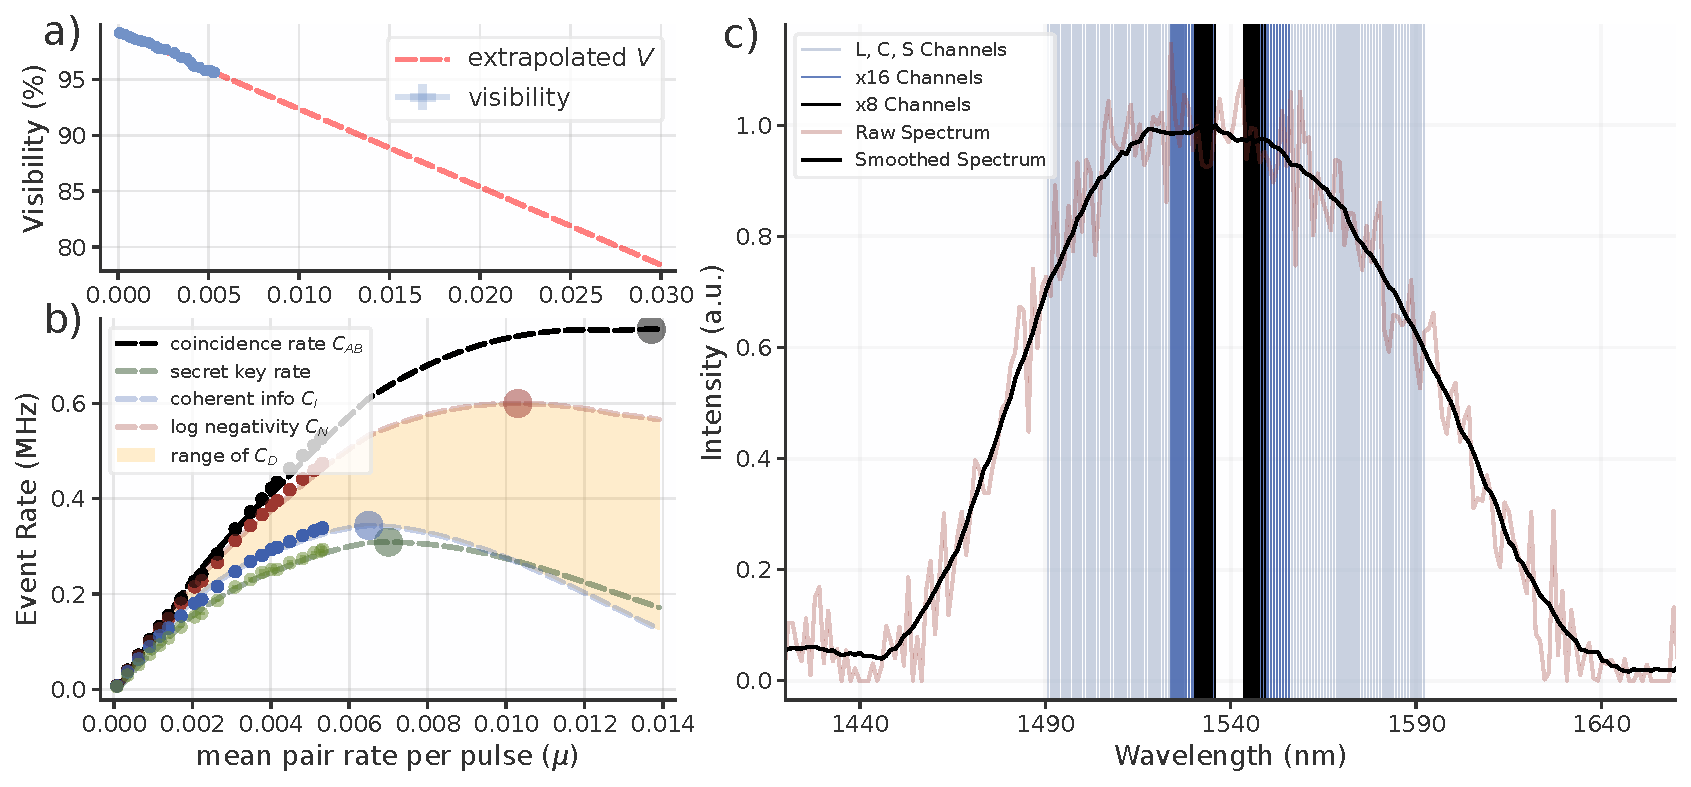
\includegraphics[width=1\linewidth]{scan_extrapolate_light.pdf}
    \caption{a) and b) include data from main text Figure 3, and extrapolate it to higher $\mu$. It is notable that $C_I$ and $SRK$ reach their maximum values for only marginally higher pump powers than those used for our measurements. c) Spectrum of entangled photon pairs out of the SPDC, measured with an Anritsu MS9740B spectrum analyzer in High Dynamic Range mode. As the signal was near the instrument noise floor, many repeated spectrum measurements were point-averaged.}
    \label{fig:scan_extrapolate}
\end{figure}

block:

\hypertarget{conclusion}{%
\chapter{Conclusion}\label{conclusion}}

\appendix

\hypertarget{aph-138-homework-assignment}{%
\chapter{Aph 138 Homework Assignment}\label{aph-138-homework-assignment}}

In March of 2022, Matthew Shaw was a guest lecturer for the Quantum Hardware and Techniques course (APh/Ph 138b). The following is a homework assignment I wrote to accompany his series of lectures.

The first problem is inspired by the low dark count rate publication~\autocite{Mueller:21}. It has the student build a simple model for a dark count rate transmitted through a series of filters. Finally, it leads the student to consider an ultimate tradeoff between dark count rate and coupling efficiency to wide bandwidth optical signals. A filtering system that only transmits a very narroband signal will not be able to detect ultra-short optical signals with high efficiency or temporal resolution.

The second problem explores a potential use case of a photon number resolving SNSPD. It closely follows logic presented in an Andreas Christ and Christine Silberhorn paper~\autocite{Andreas:12}. I studied this paper earlier in my PhD, when I considered developing a multiplexed single photon source. It turned out that project was overly ambitious, but future PhD students might consider approaching it again.

\textcolor{midnightblue}{Contact \href{mailto:andrewstermueller@gmail.com}{Andrew Mueller} with any questions about the homework or solution manual. The solutions to some sections specify finer-grained point values when there are multiple answers per section. As the grader, feel free to use these or not. }

\hypertarget{free-space-coupling-with-low-dark-counts-50-points}{%
\subsection{1. Free space coupling with low dark counts (50 points)}\label{free-space-coupling-with-low-dark-counts-50-points}}

An experimental apparatus emits a collimated beam of $1550~\mathrm{nm}$ photons with gaussian beam waist $w_0 = 3~\mathrm{mm}$. You wish to focus the beam onto an SNSPD directly through a window in a cryostat.

\hypertarget{fig:cryostat_concept}{%
\begin{figure}
\centering
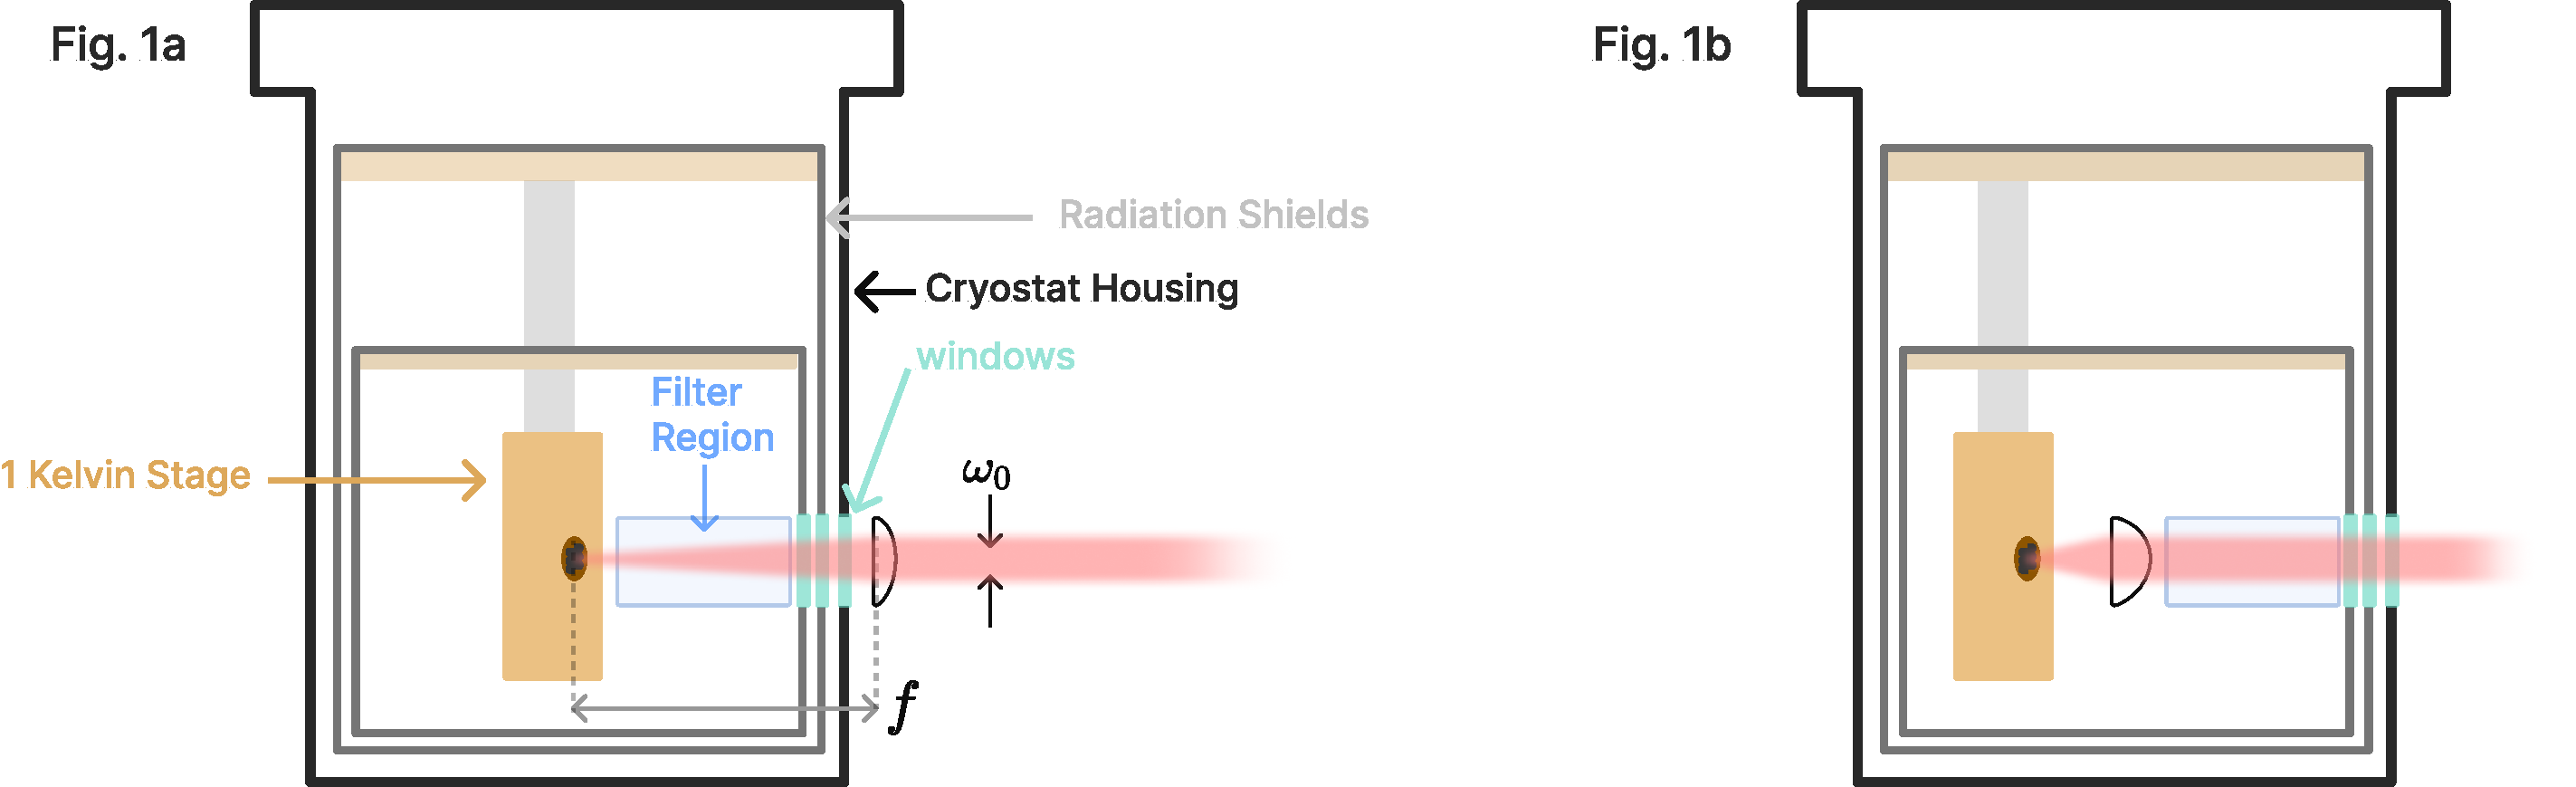
\includegraphics{./chapter_07/figs/fig1b_light.pdf}
\caption[{Cryostat optical coupling}]{\textbf{Cryostat free space coupling options.}}
\label{fig:cryostat_concept}
\end{figure}
}

As we will see later on, a set of filters will be needed between the detector and the window to minimize dark counts. In practice, the set of filters can be quite thick. Say a $f = 100~\mathrm{mm}$ lens is used right outside the cryostat to focus the beam onto the detector though a set of filters (Fig.~\ref{fig:cryostat_concept} a). The long focal length makes room for a few inches of filters between the external lens and focused spot.

\begin{enumerate}
\def\labelenumi{\arabic{enumi}.}
\item
  (4 pts)
  If the detector has a circular active area with radius $5~\mathrm{\upmu m}$, what ratio of power in the beam can it collect? Assume the detector has unity efficiency across all angles of incidence with respect to the surface normal.

  \textcolor{midnightblue}{

  \textbf{Answer:}

  }

  \textcolor{midnightblue}{

  The divergence angle of the guassian beam: $\theta = \tan^{-1}({\frac{3}{100}})$.

  }

  \textcolor{midnightblue}{ The formula for divergence angle in terms of waist $w_0$: $\theta = \frac{\lambda}{\pi w_0}$ }

  \textcolor{midnightblue}{ Combining and plugging in, the waist radius at focus is $\frac{1550~\mathrm{nm}}{\pi \tan^{-1}(\frac{3}{100})} \approx 16.5~ \mathrm{\upmu m}$ }

  \textcolor{midnightblue}{ The formula for power inside an aperture at $w(z)$ for a guassian beam:}

  \textcolor{midnightblue}{

  $$P(r, z)=P_{0}\left[1-e^{-2 r^{2} / w^{2}(z)}\right]$$

  }

  \textcolor{midnightblue}{We are interested in the ratio of power collected at $w(z=0) = w_0$ which may be expressed as:}

  \textcolor{midnightblue}{

  $$P(r, z=0)=1-e^{-2 r^{2} / w_0^{2}}$$

  }

  \textcolor{midnightblue}{Plugging in: }

  \textcolor{midnightblue}{

  $$P(r, z=0)=1-e^{-2(5^{2}) / 16.5^{2}} \approx  \boxed{0.17} $$

  }
\item
  (4 pts)
  A faster lens mounted much closer to the detector inside the cryostat focuses to a smaller waist. Consider an $f = 18~\mathrm{mm}$ lens with the detector at the focal length (Fig.~\ref{fig:cryostat_concept} b). Verify more than 99\% of the collimated light will be focused onto the active area of the detector.

  \textcolor{midnightblue}{ The waist radius at focus is $\frac{1550~\mathrm{nm}}{\pi \tan^{-1}(\frac{3}{18})} \approx 2.98~\mathrm{\upmu m}$ }

  \textcolor{midnightblue}{Ratio of power within the $10~\mathrm{\upmu m}$ radius active area: }

  \textcolor{midnightblue}{

  $$P(r, z=0)=1-e^{-2(5^{2}) / 2.98^{2}} \approx \boxed{0.996} $$

  }

  Without filtering, the mid-infrared photons coupled to the detector from the room temperature laboratory are a dominant source of dark counts. Think of the environment outside the window as an isotropic blackbody emitter. Consider 3 cases, where the shaded red regions illustrate the light field of thermal radiation that could couple to the detector:

  \hypertarget{fig:coupling_options}{%
  \begin{figure}
  \centering
  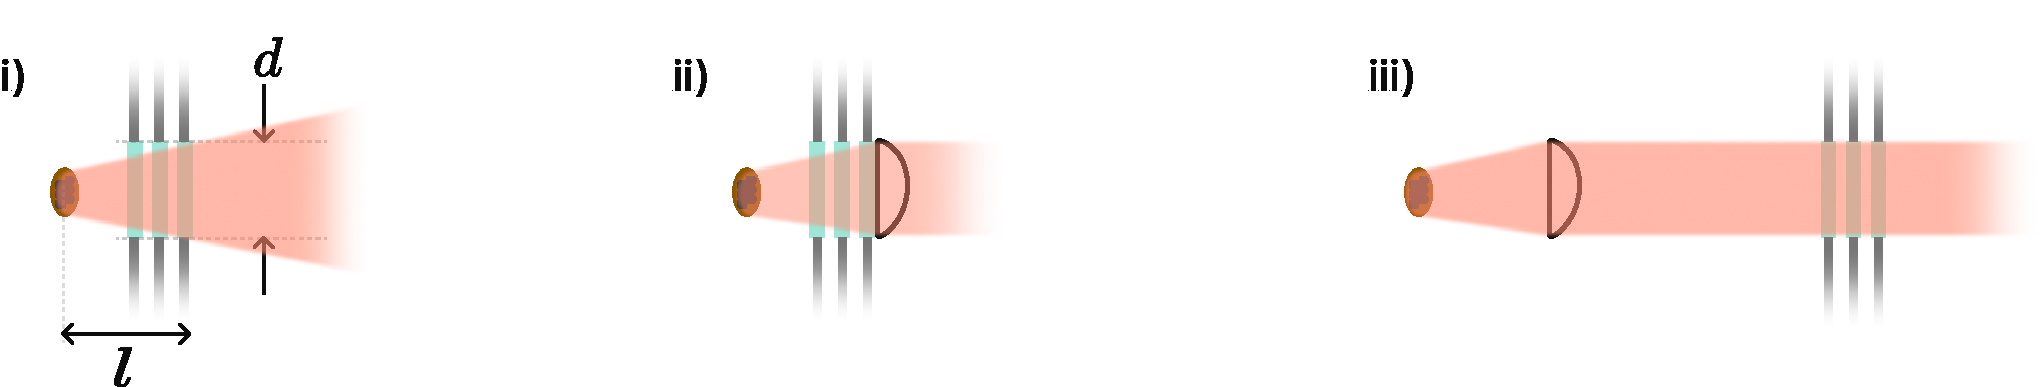
\includegraphics{./chapter_07/figs/fig2b_light.pdf}
  \caption[{Cryostat coupling options}]{\textbf{Three Coupling Options}}
  \label{fig:coupling_options}
  \end{figure}
  }

  \begin{enumerate}
  \def\labelenumii{\roman{enumii})}
  \tightlist
  \item
    There is no lens; the detector is distance $l$ inside the cryostat, and the first window with diameter $d$ defines an entrance pupil.
  \item
    Same as (i), but a lens with focal length $l$ is placed right outside the first window. The detector is at the focal point.
  \item
    Same as (ii) but the lens is placed inside the cryostat with the detector still at the focal length. Equivalent to Fig.~\ref{fig:cryostat_concept} b above.
  \end{enumerate}
\item
  (6 pts) Does (ii) couple more, less, or equal dark counts to the detector than (i)? What about case (iii)? Why? No calculations should be needed.
  (Hint: Consider the units of radiance, which characterizes a black body emitter. Etendue or beam parameter product may be useful concepts to consider)

  \textcolor{midnightblue}{ \textbf{Answer:} }
  \textcolor{midnightblue}{ The three cases couple the same amount of light to the detector. (ii) couples the same amount of power as (i) because a blackbody source can't be focused to higher intensity with a lens. The solid angle subtended by the entrance pupil as seen by the detector is the same in all cases. The detector area stays the same as well so the etendue is conserved across all three cases. This implies the same radiant power is coupled. }

  \textcolor{midnightblue}{ 3 points for saying all situations couple the same rate; 3 points for some explanation. }
\item
  (9 pts) Using Planck's law with laboratory temperature $T$ and the geometry of case (i) above, write an expression for spectral radiant flux (photons per unit wavelength) on the active area of a detector with radius $r$.

  \textcolor{midnightblue}{ \textbf{Answer:} }
  \textcolor{midnightblue}{The expression is a product of several factors:}

  \textcolor{midnightblue}{

  $$\text{Flux}[\lambda] = P \Omega D_{area} B_{\lambda}(\lambda, T)$$

  }

  \textcolor{midnightblue}{ Where $P = \frac{\lambda}{hc}$ is the number of photons per unit energy, $\Omega$ is the solid angle of blackbody radiation as seen by the detector, $D_{area} = \pi r^2$ is the area of the detector, and $B_{\lambda}$ is Planck's law. }
  \textcolor{midnightblue}{Planck's law:}

  \textcolor{midnightblue}{

  $$B_{\lambda}(\lambda, T)=\frac{2 h c^{2}}{\lambda^{5}} \frac{1}{e^{h c /\left(\lambda k_{\mathrm{B}} T\right)}-1}$$

  }

  \textcolor{midnightblue}{ $\Omega = \pi \sin{\theta^2}$, where $\theta = \tan^{-1}(\frac{(d/2)}{l})$ is the half angle of the field of view of blackbody radiation as seen by the detector. }

  \textcolor{midnightblue}{The full expression: }

  \textcolor{midnightblue}{

  $$\text{Flux}[\lambda] = \frac{\lambda \pi^2 r^2 \sin{\theta^2}}{hc} \frac{2 h c^{2}}{\lambda^{5}} \frac{1}{e^{h c /\left(\lambda k_{\mathrm{B}} T\right)}-1}, \,\,\,\,\,\,\,\,\,\,\,\theta = \tan^{-1}(\frac{(d/2)}{l})$$

  }

  \textcolor{midnightblue}{ Since the expression asked for can be written many ways, just verify the student has taken into account all the terms in equation (1) above, and has the correct expressions for} \textcolor{darkred}{$\Omega$ (3 pts), $\theta$ (3 pts), and P (3 pts).}
\item
  (6 pts) Consider the configuration in Fig. 1b). The detector has an internal quantum efficiency approximated by:

  $$\eta(\lambda) = \frac{1}{2}(1 - \text{erf}[\lambda - 3~\mathrm{\upmu m}]) $$

  $\lambda$ is measured in $\mathrm{\upmu m}$ and $\text{erf}()$ is the error function. Using your conclusions from (1.3) and expression from (1.4), write a formula $N_{photons}[\lambda]$ for the number of detectable dark counts with respect to $\lambda$, then numerically integrate it to find the dark count rate with no filtering. The laboratory temperature $T$ is 293 K, lens focal length $l$ is $18~\text{mm}$, detector radius $r$ is $5~\mathrm{\upmu m}$, and the diameter $d$ of all optics is 1 inch. The maximum count rate of this SNSPD is 10 MHz. Is the detector usable or overexposed?

  \textcolor{midnightblue}{ \textbf{Answer:} }
  \textcolor{midnightblue}{Use the expression from (1.4) and multiply it by the quantum efficiency function $\eta(\lambda)$ }

  \textcolor{midnightblue}{

  $$N_{photons}[\lambda] = P \Omega D_{area} \eta(\lambda) B_{\lambda}(\lambda, T=293)$$

  }

  \textcolor{midnightblue}{ Here is the function expressed in mathmatica and the solution to the integral: }

  \textcolor{midnightblue}{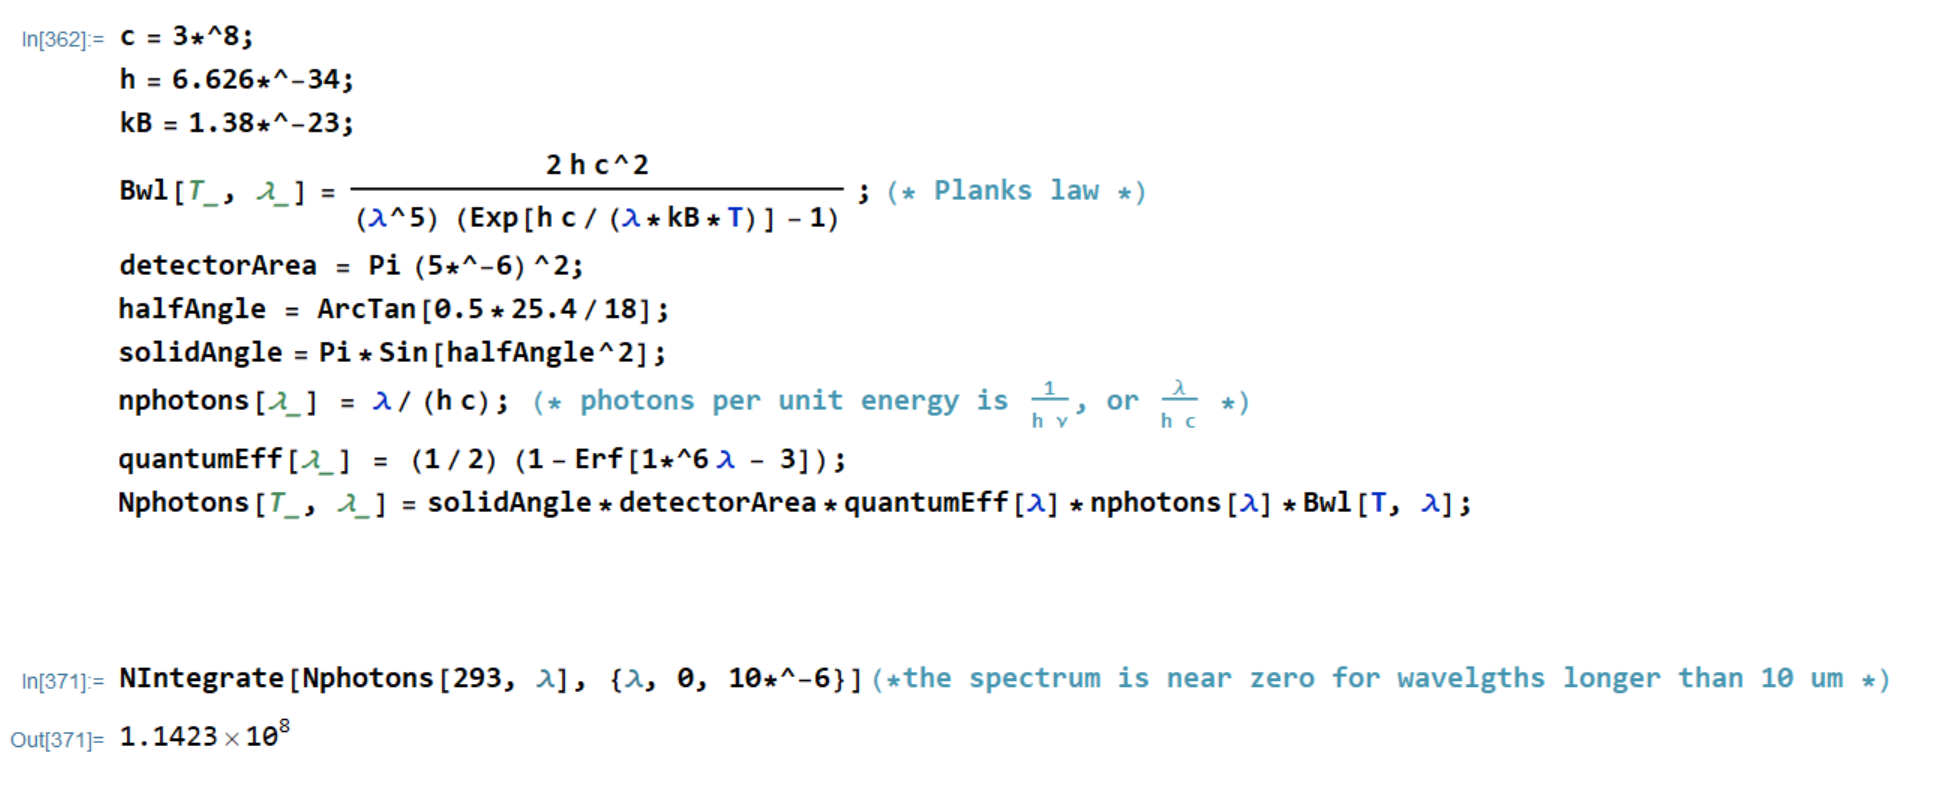
\includegraphics{./chapter_07/figs/mathematica_2.PNG}}

  \textcolor{midnightblue}{Dark count rate $\approx \boxed{110 \,\text{MCounts/s}}$ }
  \textcolor{midnightblue}{The rate of dark counts exceeds the usual maximum count rate, the detector is not usable. }

  \textcolor{midnightblue}{3 pts. for similar dark count rate (+/- 20\%) , 3 pts. for saying the detector is not usable.}
\item
  (6 pts) A set of shortpass filters can remove the bulk of blackbody radiation. A shortpass filter can be roughly modeled with the formula:

  $$F(\lambda, E_t) = \frac{1}{E_t}[(E_t - 1)H(\lambda_c - \lambda) + 1]$$

  Where H is the Heaviside step function, $\lambda_c$ is the cutoff wavelength of the filter, and $E_t$ is the extinction ratio of the filter. Use this with $N_{photons}[\lambda]$ from (d). How many filters with $\lambda_c = 1560~\text{nm}$ and $E_t = 30~\text{dB}$ are necessary to suppress the spectral region of detectable dark counts longer than 1560 nm so that it is not the dominant source of dark counts?

  \textcolor{midnightblue}{ \textbf{Answer:} }

  \textcolor{midnightblue}{$\boxed{\text{3 filters}}$ are needed to make the wavelength band shorter than 156 nm the dominant source of counts.} \textcolor{darkred}{3 pts. for this answer}

  \textcolor{darkred}{3 pts for evidence:}
  \textcolor{midnightblue}{Students might integrate the detectable dark count spectrum with different numbers of filters and comparing the results. The computations below show the addition of a fourth filter has a negligible effect on the dark count rate. }

  \textcolor{midnightblue}{Students may instead give a more qualitative answer, for example with a graph of the filtered spectrums, that shows the relative suppression of the region longer than 1560 nm. }

  \textcolor{midnightblue}{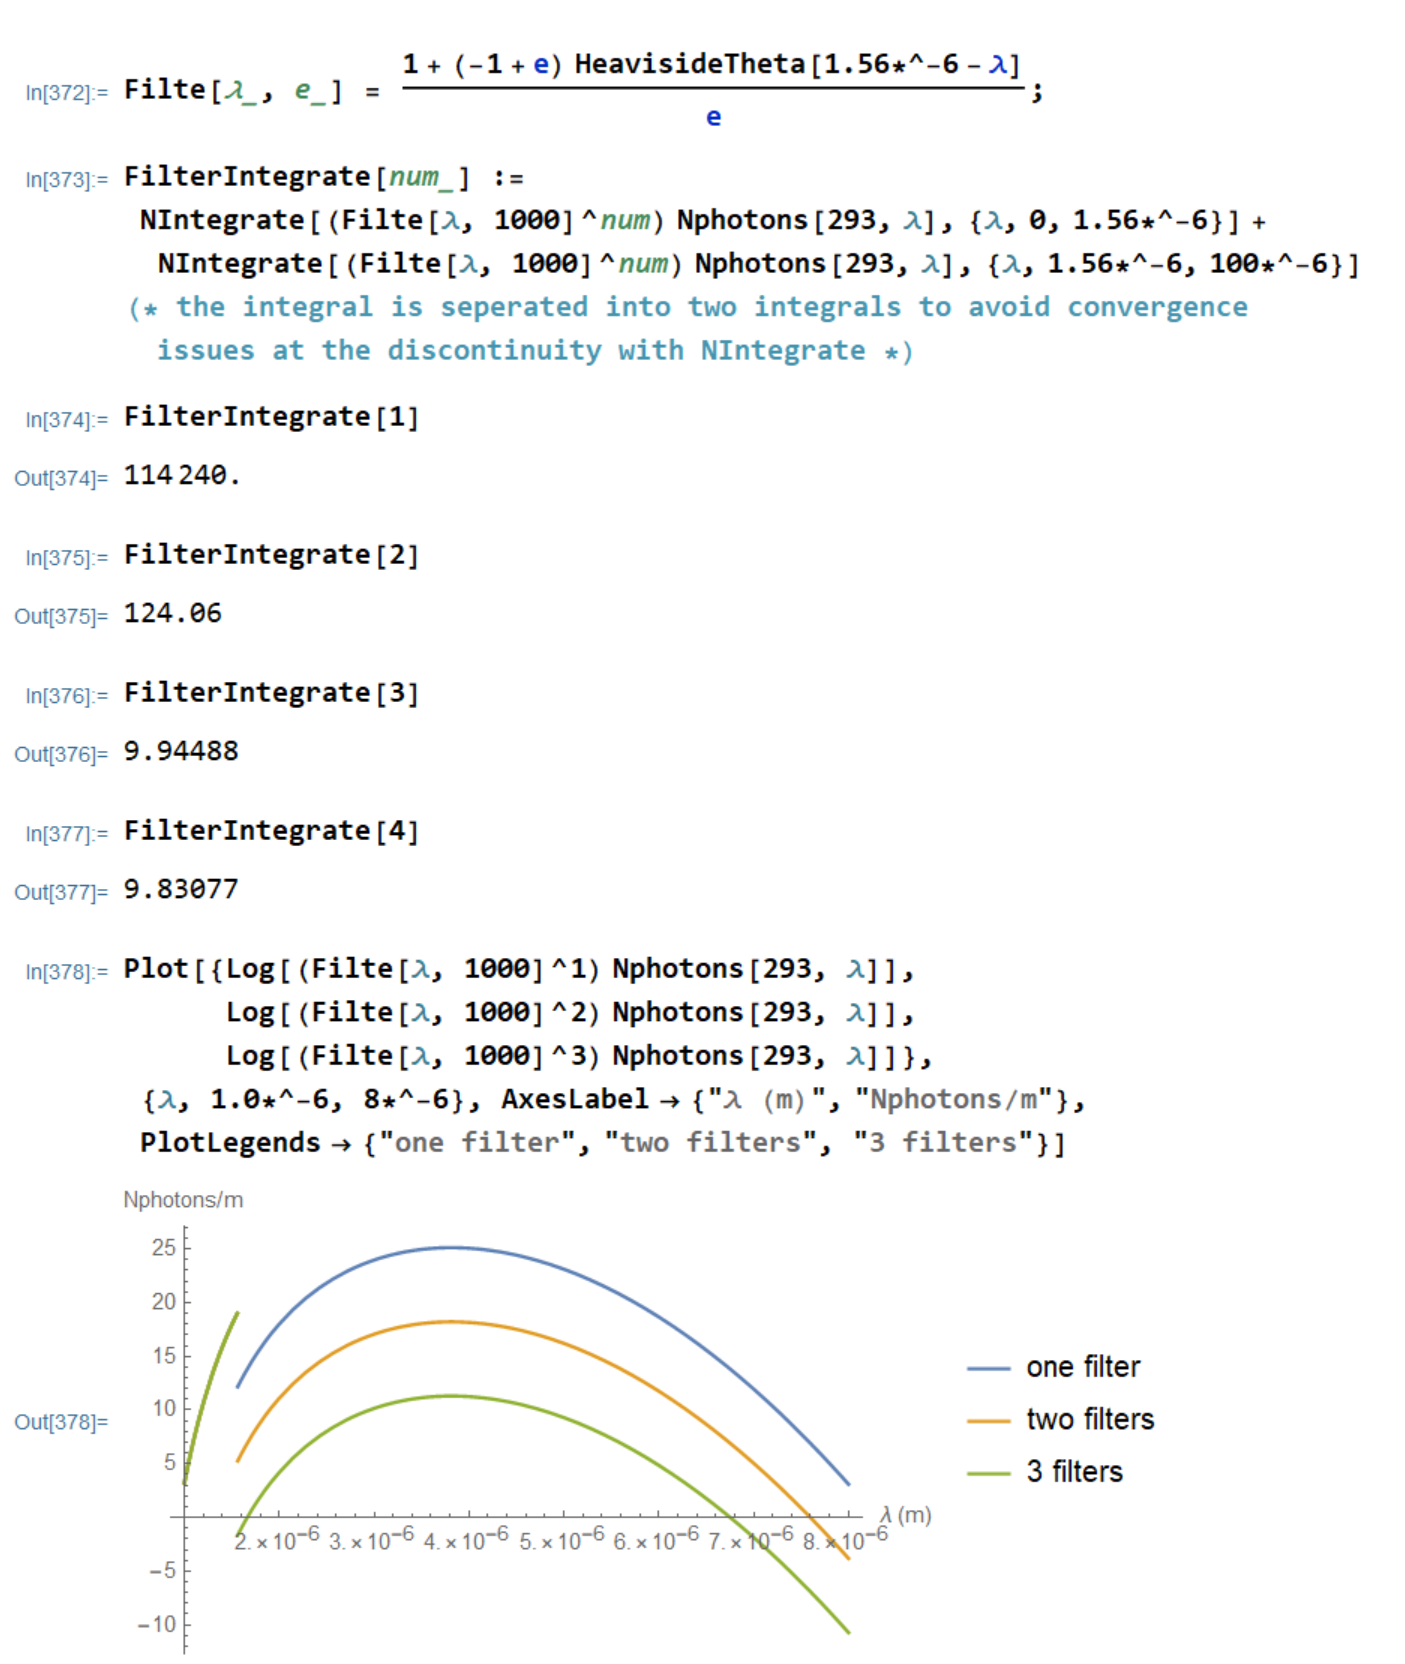
\includegraphics{./chapter_07/figs/filter_integrate_4.PNG}}
\item
  (7 pts) If a narrow band filter is also inserted with center wavelength $1550~\text{nm}$ and spectral width below $1-2~nm$, then dark count rate can be approximated as just $N_{photons}[\lambda = 1550~\text{nm}]$ times the filter width. Show for this wavelength range you can simplify dark count rate further to a simple exponential function. If the laboratory air conditioner breaks, raising the lab temperature from 293 K to 300 K, how much higher is the dark count rate?

  \textcolor{midnightblue}{ \textbf{Answer:} }

  \textcolor{midnightblue}{The expression for $N_{photons}[\lambda]$ from part (1.4) can be simplified and evaluated at 1550 nm, then multiplied by the filter width in nanometers. }

  \textcolor{midnightblue}{

  $$\begin{aligned}
   N_{photons}[\lambda] &= P \Omega D_{area} \eta(\lambda) B_{\lambda}(\lambda) \\
   N_{filter} &= N_{photons}[\lambda = 1550~\text{nm}]\Delta \lambda
   \end{aligned}$$

  }

  \textcolor{midnightblue}{This code shows integrating the spectrum and just multiplying $N_{photons}$ times the filter width produce very similar results (for a 1 nm filter):}

  \textcolor{midnightblue}{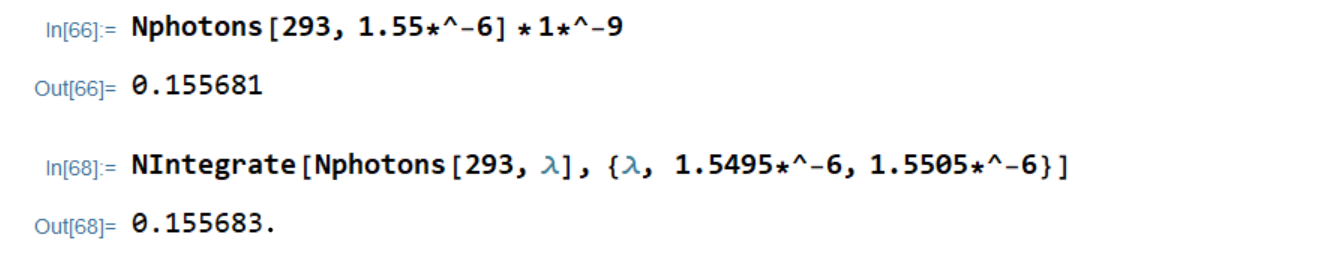
\includegraphics{./chapter_07/figs/nphoton_approx.PNG}}

  \textcolor{midnightblue}{Evaluating the $N_{photon}$ function at $\lambda = 1550~text{nm}$ shows the $-1$ term is small relative to the exponential term:}

  \textcolor{midnightblue}{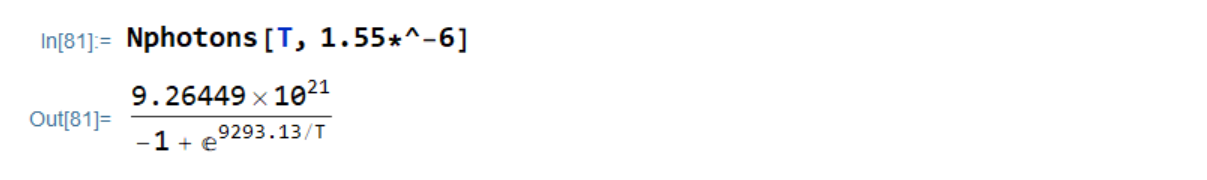
\includegraphics{./chapter_07/figs/small_relative_to_exponential.PNG}}

  \textcolor{midnightblue}{Therefore the filter transmission approximation is:}

  \textcolor{midnightblue}{

  $$\boxed{N_{filter} \approx 9.26\mathrm{e}21 \Delta\lambda e^{-9290/T} (\frac{\text{photons}}{\text{s*meter}})}$$

  }

  \textcolor{midnightblue}{or equivalently: }

  \textcolor{midnightblue}{

  $$\boxed{N_{filter} \approx 9.26\mathrm{e}12 \Delta\lambda e^{-9290/T} (\frac{\text{photons}}{\text{s*nm}})}$$

  }

  \textcolor{midnightblue}{and the dark count rate in the 300 K room is roughly double the rate in the 293 K room: }

  \textcolor{midnightblue}{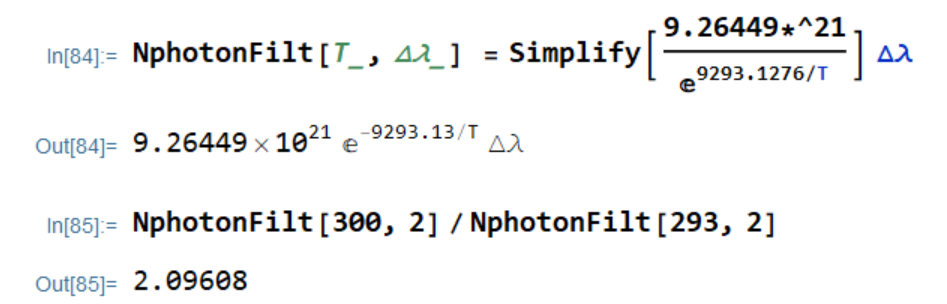
\includegraphics[width=0.6\textwidth,height=\textheight]{./chapter_07/figs/filter_with_temp.PNG}}

  \textcolor{midnightblue}{4 pts for a similar equation, 3 pts for finding the dark count rate roughly doubles. }

  A quantum communication experiment requires time-tagging photons with respect to a 50 GHz clock with 95\% fidelity. That is, 95\% of the timing measurements of detected photons emitted at the same time with respect to a clock fall within a 20 ps bin. Say the detector and readout electronics have a combined jitter of 10 ps FWHM, and a mode locked laser is used for the experiment that generates transform-limited Gaussian pulses. You tune it's temporal length to a value for which the total timing uncertainty of time-tagged photons --- including system jitter and pulse temporal length --- matches the 95 \% fidelity at 50 GHz requirement. Assume detector jitter has a Gaussian shape as well.
\item
  (8 pts) Find the spectral width of a filter that would transmit 95\% of the photons from the mode locked laser. What is the dark count rate with this filter, using the expression from (1.7) and T = 293 K?

  \textcolor{midnightblue}{ \textbf{Answer:} }

  \textcolor{midnightblue}{For transform limited guassian pulses, the product of temporal and spectral width at a FWHM level is \href{https://www.lasercalculator.com/transform-limited-pulse-calculator/}{about 0.441}. There's a derivation of this \href{https://www.physicsforums.com/threads/time-bandwidth-product-ideal-mode-locking.171404/post-1339948}{here}, but students don't need to show it. }

  \textcolor{midnightblue}{

  $$T B P_{\text {Gaussian }}=\frac{2 \log 2}{\pi} \approx 0.441$$

  }

  \textcolor{midnightblue}{ Since this uses the FWHM level, all the 95\% metrics need to be converted. About 95\% of the area under a guassian falls within $\pm 2 \sigma$. }

  \textcolor{midnightblue}{ Bound on total system timing uncertainty: $20~\text{ps}_{95\%} = (20/4)*2.35 = 11.75~\text{ps}_{FWHM}$ }

  \textcolor{midnightblue}{ The jitter of the detection system and the temporal width of the laser pulse $\Delta t$ should add in quadrature to match the bound: }

  \textcolor{midnightblue}{

  $$ 11.75~\text{ps}_{FWHM} = \sqrt{ \Delta t^2 + (10~\text{ps})^2}$$

  }

  \textcolor{midnightblue}{

  $$\begin{aligned}
   0.441 = \Delta t \Delta \nu \\
   \Delta \nu = 71~\text{GHz} \\
   \Delta \lambda = \frac{\lambda^2 \Delta \nu}{c} = 0.57~\text{nm} \\
   \end{aligned}$$

  }

  \textcolor{midnightblue}{ $0.57~\text{nm}$ is the spectral width of the laser pulse at the FWHM level. If this pulse passes through a tophat filter with width equal to the 95\% level of the laser pulse, then 95\% will be transmitted. }

  \textcolor{midnightblue}{Filter width: }

  \textcolor{midnightblue}{

  $$\Delta \lambda_{95\%} = \frac{4 \Delta \lambda}{2.35} \approx \boxed{1~\text{nm}} $$

  }

  \textcolor{midnightblue}{Dark count rate is easy to find using the expression from the previous section: }

  \textcolor{midnightblue}{

  $$\boxed{N_{filter} \approx 9.26e12 (1~\text{nm}) e^{-9290/T} (\frac{\text{photons}}{\text{s*nm}})} \approx 0.15~\text{photons/s} $$

  }

  \textcolor{midnightblue}{3 points for writing and solving the equation that matches the jitter bound to the quadrature sum }
  \textcolor{midnightblue}{5 points for correct filter width and dark count rate}
\end{enumerate}

\hypertarget{spdc-coupling-and-single-photon-sources-50-points}{%
\subsection{2. SPDC Coupling and Single Photon Sources (50 points)}\label{spdc-coupling-and-single-photon-sources-50-points}}

A Spontaneous Parametric Down Conversion (SPDC) crystal is known to generate a twin beam squeezed state of the form:

$$|\psi\rangle= \sqrt{1 - \gamma^2} \sum_{n=0}^{\infty} \gamma^{n}\left|n_{s}, n_{i}\right\rangle $$

Where $n_s$ and $n_i$ are the number of photons corresponding to the signal and idler parts of the wavefunction. Consider Fig.~\ref{fig:hsps} a, where the crystal is pumped with a pulsed laser, and the the signal and idler components that emerge are separated either by polarization or frequency. The idler arm is sent to an SNSPD. This configuration can be used as a heralded single photon source (HSPS). A click on the detector on the idler arm `heralds' a non-vacuum state in the signal arm. High fidelity and probability single photon sources are very useful for various quantum optics experiments and technologies, including linear optical quantum computing.

\hypertarget{fig:hsps}{%
\begin{figure}
\centering
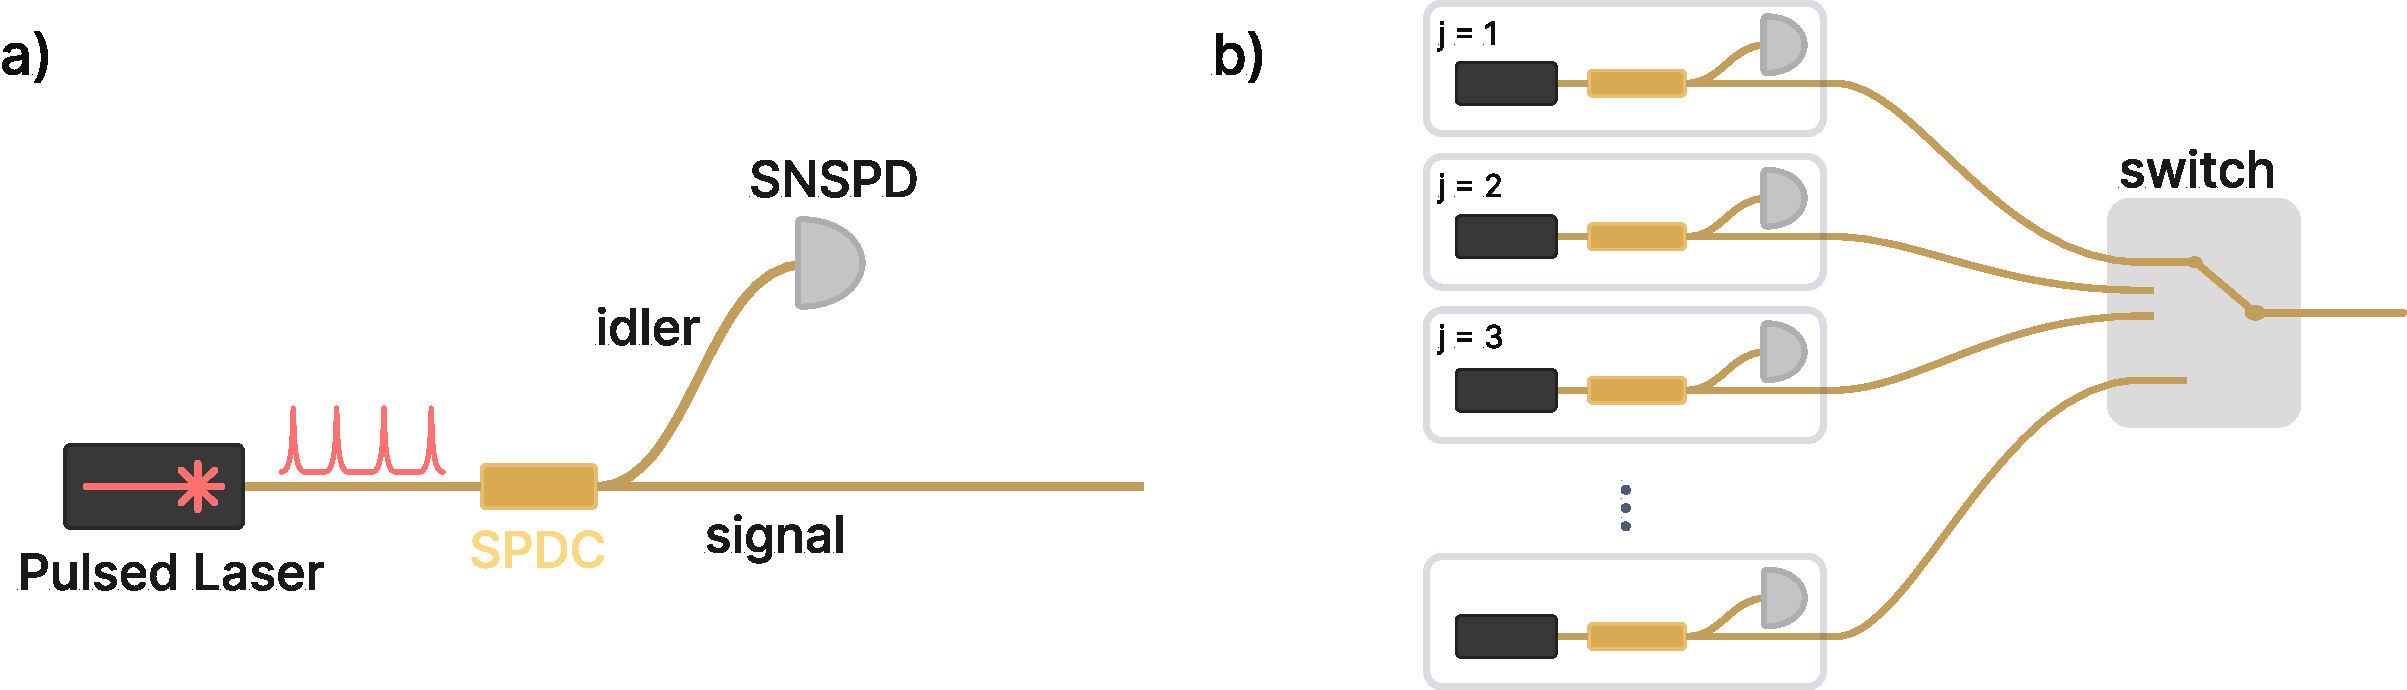
\includegraphics{./chapter_07/figs/hsps_light.pdf}
\caption[{Heralded single photon source designs}]{\textbf{Heralded single photon sources}}
\label{fig:hsps}
\end{figure}
}

Most SNSPDs are \emph{binary}-type single photon detectors, meaning they differentiate between zero and one or more photons arriving in a given light pulse. A positive operator value measure (POVM) quantifies how a `click' from a binary SPD updates our knowledge of the incident state:

$$\hat{\Pi}_{\text {binary}} = \sum_{n=0}^{\infty}\left[1-(1-\eta)^{n}\right]|n\rangle\langle n|$$

Where $\eta$ is the coupling efficiency between the state of interest and the detector.

\begin{enumerate}
\def\labelenumi{\arabic{enumi}.}
\item
  (6 pts) Find the expectation value of $\hat{\Pi}_{\text {binary}}$ given the SPDC state above. This is the probability $p_{binary}\left(\gamma, \eta\right)$ of getting a binary detector click on the idler arm. For $\gamma << 1$, what is $p_{binary}$ up to lowest order in $\gamma$, and what fock state of the signal arm is the source of this dominant term?

  \textcolor{midnightblue}{ \textbf{Answer:} }

  \textcolor{midnightblue}{

  $$\begin{aligned}
   \langle \psi | \Pi_{\text {binary}} | \psi \rangle &= (1- \gamma^2) \sum_{\tilde{n}=0}^{\infty} \langle \tilde{n}_s \tilde{n}_i | \gamma^{\tilde{n}} \sum_{n=0}^{\infty}[1 - (1-\eta)^{n}] \gamma^n | n_s n_i \rangle \\
   \langle \psi | \Pi_{\text {binary}} | \psi \rangle &= p_{binary}(\gamma, \eta) =  \boxed{(1-\gamma^2) \sum_{n_s=0}^{\infty} \gamma^{2n_s} [1 - (1 - \eta)^{n_s}]}
   \end{aligned}$$

  }

  \textcolor{midnightblue}{For $\gamma << 1, ~~ p \sim (1 - \gamma^2)[\cancel{\gamma^0[1 - (1 - \eta)^0]} + \gamma^{2}\eta ] \sim (1 - \gamma^2)\gamma^{2}\eta$ }

  \textcolor{midnightblue}{ To lowest order in $\gamma$, $p \sim \gamma^{2}\eta$. The single photon fock state dominates for $\gamma << 1$. }

  \textcolor{midnightblue}{ 3 pts for correct $p_{binary}(\gamma, \eta)$; 3 pts for saying the leading term is from single photons }
\item
  (6 pts) A general form for the density matrix of the signal mode given a herald event is:

  $$\rho_{s}\left(\gamma, \eta\right)=\frac{\operatorname{Tr}_{i}\left(\hat{\Pi}|\psi\rangle\langle\psi|\right)}{\left\langle\psi\left|\hat{\Pi}\right| \psi\right\rangle}$$

  Write down the $|1\rangle\langle1|$ term of this matrix, and simplify any infinite sums. This is the single photon fidelity $F_{binary}(\gamma, \eta)$. Why does $F_{binary}$ approach zero for $\gamma$ approaching 1? What types of states is the SPDC generating in this limit?

  \textcolor{midnightblue}{ \textbf{Answer:} }

  \textcolor{midnightblue}{

  $$\begin{aligned}
   \rho_s(\gamma,\eta) &= \frac{\operatorname{Tr}_i[\cancel{(1 - \gamma^2)}\Sigma_{n=0}^{\infty} \gamma^{2n}[1 - (1 - \eta)^{n} ]| n \rangle \langle n | n_s n_i \rangle \langle n_s n_i |]}
   {\cancel{(1-\gamma^2)} \sum_{n_s=0}^{\infty} \gamma^{2n_s} [1 - (1 - \eta)^{n_s}]}\\
   |1_s \rangle \langle 1_s | &= \frac{\gamma^2[1 - (1 - \eta)]}{\sum_{n_s=0}^{\infty} \gamma^{2n_s} [1 - (1 - \eta)^{n_s}]} = \frac{\gamma^2 \eta}{\sum_{n_s=0}^{\infty} \gamma^{2n_s} [1 - (1 - \eta)^{n_s}]}\\
   |1_s \rangle \langle 1_s | &= \frac{\gamma^2 \eta}{\sum_{n_s=0}^{\infty}(\gamma^{2n_s} - [\gamma^2 (1 - \eta)]^{n_s})}\\
   &= \frac{\gamma^2 \eta}{\frac{1}{1 - \gamma^2} - \frac{1}{1 - \gamma^2(1 - \eta)}}\\
   &= \frac{\gamma^2 \eta (1 - \gamma^2)}{1 - \frac{1 - \gamma^2}{1 - \gamma^2(1 - \eta)}}\\
   &= \frac{\cancel{\gamma^2 \eta} (1 - \gamma^2) (1 - \gamma^2 (1 - \eta))}{\cancel{1 - \gamma^2 (1 - \eta) - 1 + \gamma^2}} \\
   F_{binary}(\gamma, \eta) &= \boxed{(1 - \gamma^2)(1 - \gamma^2(1 - \eta))}
   \end{aligned}$$

  }

  \textcolor{midnightblue}{As $\gamma$ approaches 1, the denominator in the original expression for $\rho_s(\gamma,\eta)$ approaches infinity while the numerator approaches $\eta$. In this limit, the SPDC is generating predominantly multi-photon states. For $\gamma$ approaching 1, the probability of the generated state being a single photon state goes to zero. Because the binary POVM was used, multi-photon states are `included' in $\rho_s(\gamma,\eta)$. For $\rho_s$ from the PNR POVM shown below, multi-photon states will be included to a much lesser extent, depending on the value for $\eta$.}

  \textcolor{midnightblue}{3 pts for correct $F_{binary}(\gamma, \eta)$; 3 pts for similar explanation}

  An HSPS with high single photon fidelity and probability is most useful, but you see these metrics are maximized for opposite limits of $\gamma$. One approach to achieving high probability and fidelity simultaneously is to link multiple SPDC sources and heralding detectors as shown in Fig.~\ref{fig:hsps} b. A click from the detector $j$ triggers the switch to move to position $j$ and let the heralded state pass through. This way, $\gamma$ for each source can be kept low to maximize fidelity, while heralding probability increases with the number of sources.
\item
  (6 pts) If such a multiplexing setup is engineered to have 98\% single photon fidelity from each source and 98\% heralding probability overall, how many sources and binary SNSPDs are needed? Use an idler arm efficiency $\eta$ of 80\%.

  \textcolor{midnightblue}{ \textbf{Answer:} }

  \textcolor{midnightblue}{The fist step is to determine the pump power $\gamma$ for which fideltiy is 98\%. }

  \textcolor{midnightblue}{

  $$0.98 = F_{binary}(\gamma, \eta) = (1 - \gamma^2)(1 - \gamma^2(1 - \eta)\,\,\,\,\,\,\,\, \eta = 0.8$$

  }

  \textcolor{midnightblue}{ A numerical solution is fine. We're interested in the positive solution less than one:}

  \textcolor{midnightblue}{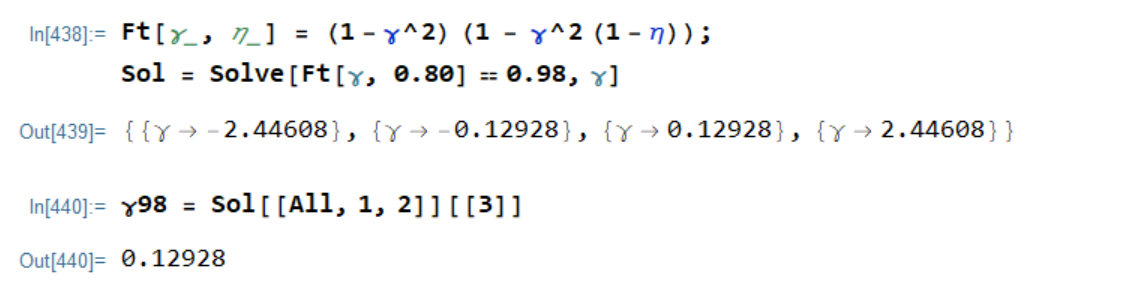
\includegraphics[width=0.7\textwidth,height=\textheight]{./chapter_07/figs/Ftsolve.PNG}}

  \textcolor{midnightblue}{Like in introductory statistics problems, its helpful to think about the negative case: Given N sources with herald probability $p$, the probability of zero sources heralding is:}

  \textcolor{midnightblue}{

  $$P(\text{no herald}|N) = (1 - p_{binary}\left(\gamma, \eta\right))^N$$

  }

  \textcolor{midnightblue}{Then the probability of at least one herald is 1 minus the previous expression:}

  \textcolor{midnightblue}{

  $$P(\text{at least one herald}|N) = 1 - (1 - p_{binary}\left(\gamma, \eta\right))^N$$

  }

  \textcolor{midnightblue}{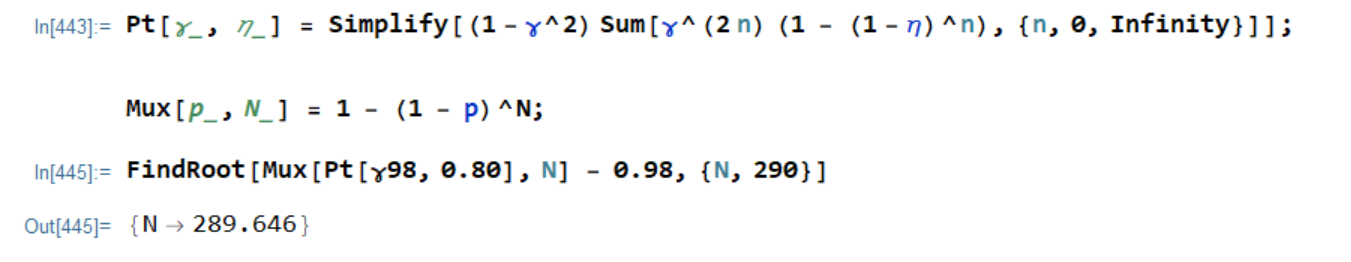
\includegraphics[width=0.7\textwidth,height=\textheight]{./chapter_07/figs/mux_binary.PNG}}

  \textcolor{midnightblue}{About $\boxed{N = 290}$ sources are needed.}

  \textcolor{midnightblue}{3 pts for correct form of the multiplexing expression
  $P(\text{at least one herald}|N)$; 3 pts for similar number of sources $N$}
\end{enumerate}

A photon number resolving (PNR) SNSPD is able to discriminate the number of photons in a light pulse*. By heralding the idler mode with a PNR SNSPD, the generation of multi-photon signal pulses can be identified and discarded. There's a POVM for an ideal PNR single photon detector, where $i$ is the number of photons detected**:

$$\hat{\Pi}_{PNR}(i)=\sum_{n=i}^{\infty}\binom{n}{i}(1-\eta)^{n-i} \eta^{i}|n\rangle\langle n|$$

\begin{enumerate}
\def\labelenumi{\arabic{enumi}.}
\setcounter{enumi}{3}
\item
  (12 pts) Derive a herald probability $p_{PNR}$ and fidelity $F_{PNR}$ for the PNR POVM, following the steps in the previous sections with $i$ set to 1. You can use symbolic math tools to simplify them if you wish. The probability of successfully heralding states in the signal arm $p_{PNR}$ should now approach zero for $\gamma$ near one. Why is this?

  \textcolor{midnightblue}{ \textbf{Answer:} }
  \textcolor{midnightblue}{The POVM for one photon detected:}

  \textcolor{midnightblue}{

  $$\hat{\Pi}_{PNR}(1)=\sum_{n=1}^{\infty}n(1-\eta)^{n-1} \eta|n\rangle\langle n|$$

  }

  \textcolor{midnightblue}{First, derive the probability of getting a single photon detection from the PNR detector: $p_{PNR}(\gamma, \eta)$:}

  \textcolor{midnightblue}{

  $$\begin{aligned}
       p_{PNR}(\gamma, \eta) =\langle \psi | \Pi_{\text {PNR}} | \psi \rangle &= (1- \gamma^2) \sum_{\tilde{n}=0}^{\infty} \langle \tilde{n}_s \tilde{n}_i | \gamma^{\tilde{n}} \sum_{n=1}^{\infty}n(1-\eta)^{n-1} \eta|n\rangle\langle n| | n_s n_i \rangle \\
       \langle \psi | \Pi_{\text {PNR}} | \psi \rangle &= p_{PNR}\left(\gamma, \eta\right) =  \boxed{(1-\gamma^2) \sum_{n_s=0}^{\infty} \gamma^{2n_s} n_s(1-\eta)^{n_s-1}}\\
       p_{PNR}\left(\gamma, \eta\right) &=  \boxed{\frac{\gamma ^2 (1 - \gamma ^2) \eta }{(\gamma ^2 (\eta -1)+1)^2}}
   \end{aligned}$$

  }

  \textcolor{midnightblue}{Where either of the boxed answers are acceptable, and the last line was found using mathematica:}

  \textcolor{midnightblue}{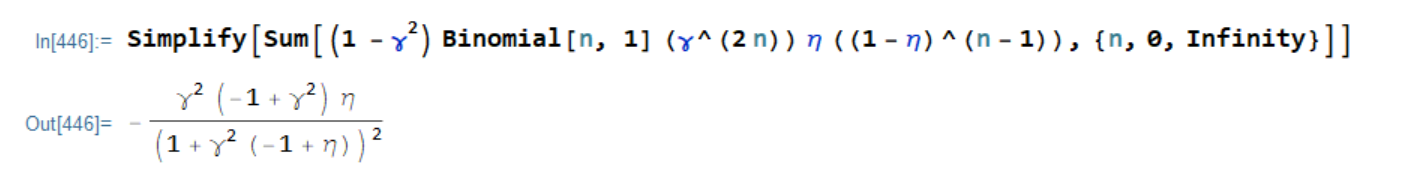
\includegraphics{./chapter_07/figs/simplify_ppnr.PNG}}

  \textcolor{darkred}{4 pts for $p_{PNR}\left(\gamma, \eta\right)$}

  \textcolor{midnightblue}{Second, derive the single photon fidelity, staring with the density matrix for the signal photon given a PNR herald event. Using (15) above for $\langle \psi | \Pi_{\text {PNR}} | \psi \rangle$ in the denominator helps simplify it significantly. }

  \textcolor{midnightblue}{

  $$\begin{aligned}
       \rho_s(\gamma,\eta) &= \frac{\operatorname{Tr}_i[\sum_{n=1}^{\infty} \gamma^{2n}n(1-\eta)^{n-1} \eta|n\rangle\langle n|n_s n_i \rangle \langle n_s n_i |]}
           {\langle \psi | \Pi_{\text {PNR}} | \psi \rangle}\\
           |1_s \rangle \langle 1_s | &= \frac{\cancel{(1 - \gamma^2)}(\gamma ^2 (\eta -1)+1)^2 \cancel{\gamma^2 \eta}}{\cancel{\gamma^2 \eta} \cancel{(1 - \gamma ^2)} }\\
           F_{PNR}(\gamma, \eta) &= \boxed{(\gamma ^2 (\eta -1)+1)^2}
   \end{aligned}$$

  }

  \textcolor{midnightblue}{4 pts for $F_{PNR}(\gamma, \eta)$}

  \textcolor{midnightblue}{For $\gamma$ near one, the SPDC is under strong pump power and is generating predominantly multi-pair states. A vanishing fraction of those states are single photon states that the PNR detector is able to distinguish and single-photon. Therefore, the PNR detector is signaling the generation of multi-pair states most of the time which should be discarded and do not contribute to $p_{PNR}$. For high efficiency $\eta$, only the vanishing single-pair creation rate contributes predominantly to $p_{PNR}$.}

  \textcolor{darkred}{4 pts for similar explanation}
\item
  (12 pts) Make a parametric plot for $0<\gamma<1$ with $F_{PNR}$ on the x-axis and $p_{PNR}$ on the y-axis. Plot the curve for a few different values of idler arm efficiency $0<\eta<1$. All curves should reach the same maximum herald probability. What is it?

  \textcolor{midnightblue}{ \textbf{Answer:} }

  \begin{center}

  \textcolor{midnightblue}{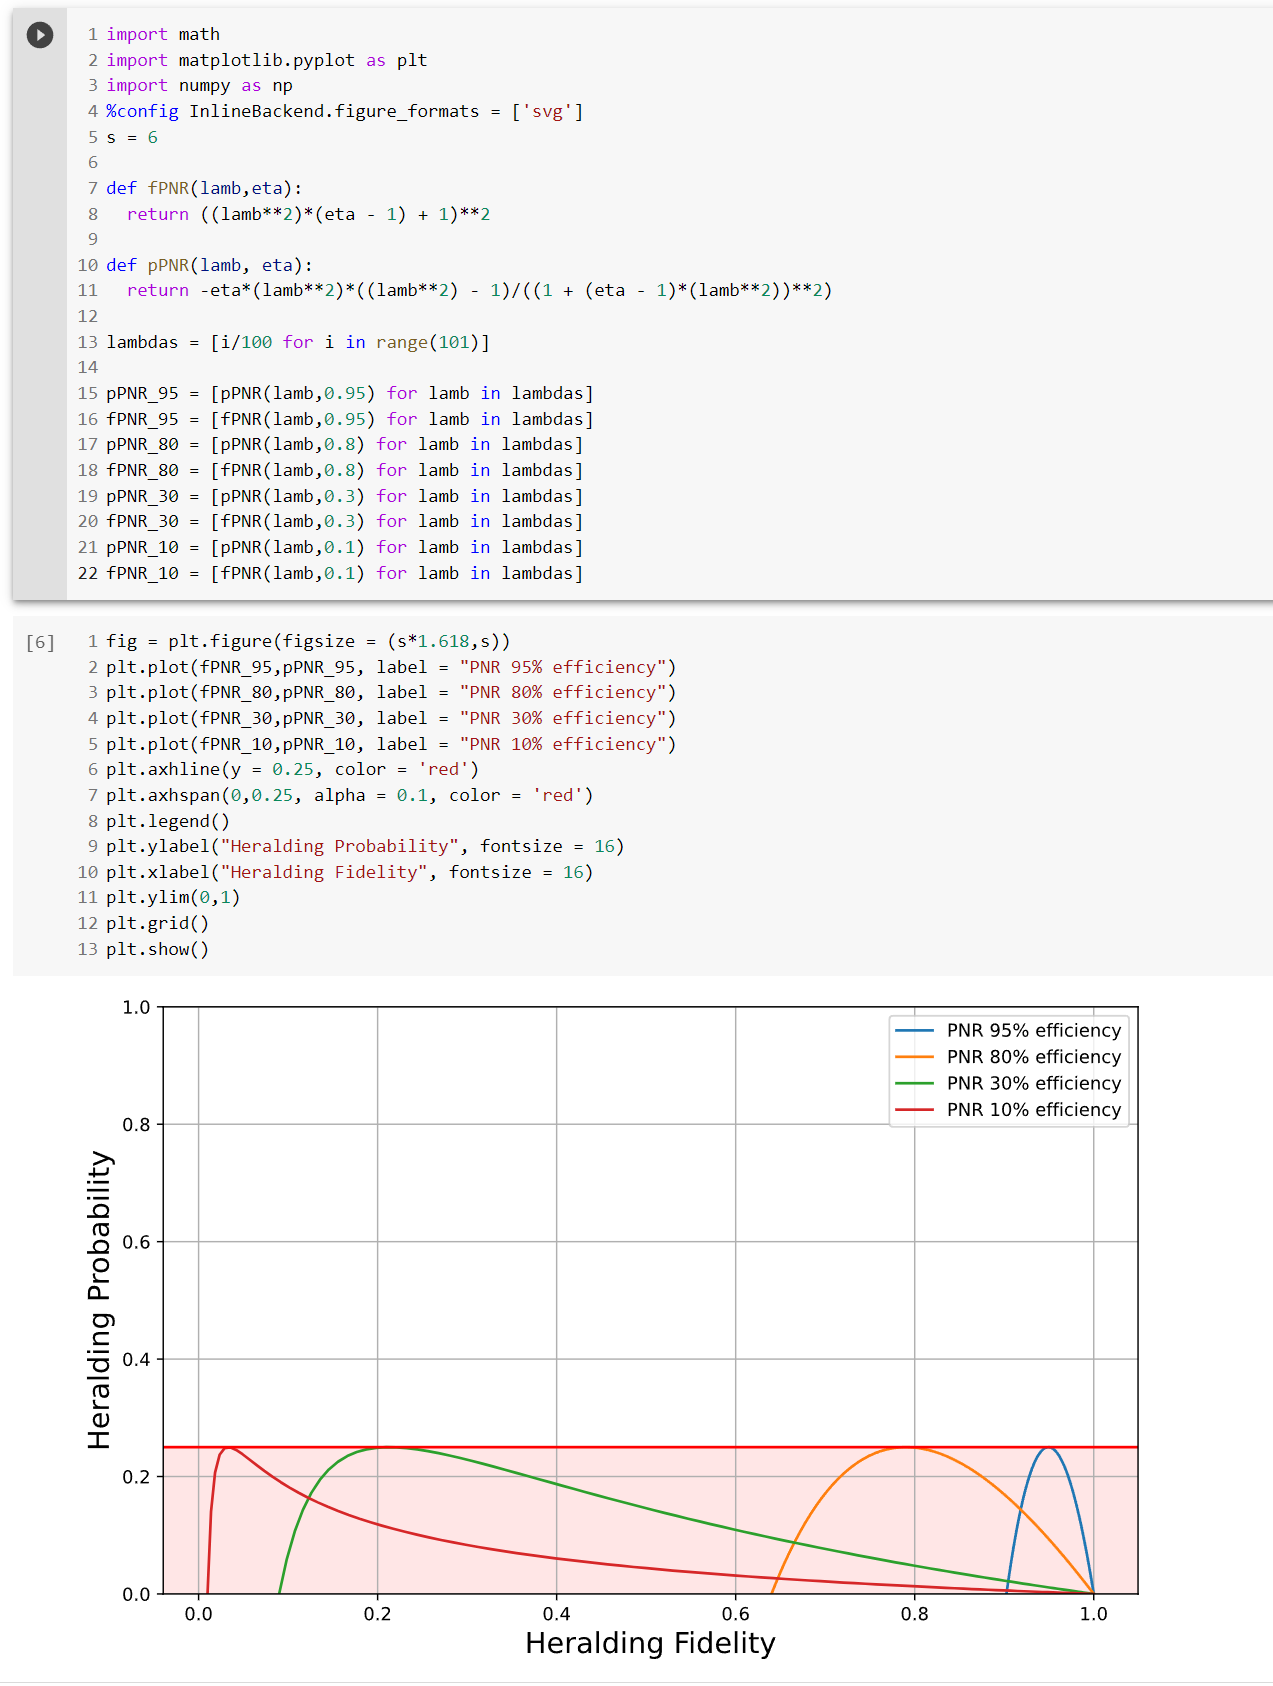
\includegraphics[width=0.7\textwidth,height=\textheight]{./chapter_07/figs/PLT.PNG}}

  \end{center}

  \textcolor{midnightblue}{ The the herald probability regardless of idler arm efficiency is 25\%. }

  \textcolor{darkred}{ 4 points for the 25\% limit; 8 points for a few plots at different $\eta$ }
\item
  (8 pts) Consider again the configuration in Fig.~\ref{fig:hsps} b. Find the number of sources using PNR detectors needed to reach 98\% single photon herald probability and fidelity with $\eta = 0.8$. Also find the number of sources for $\eta = 0.95$.

  \textcolor{midnightblue}{ \textbf{Answer:} }
  \textcolor{midnightblue}{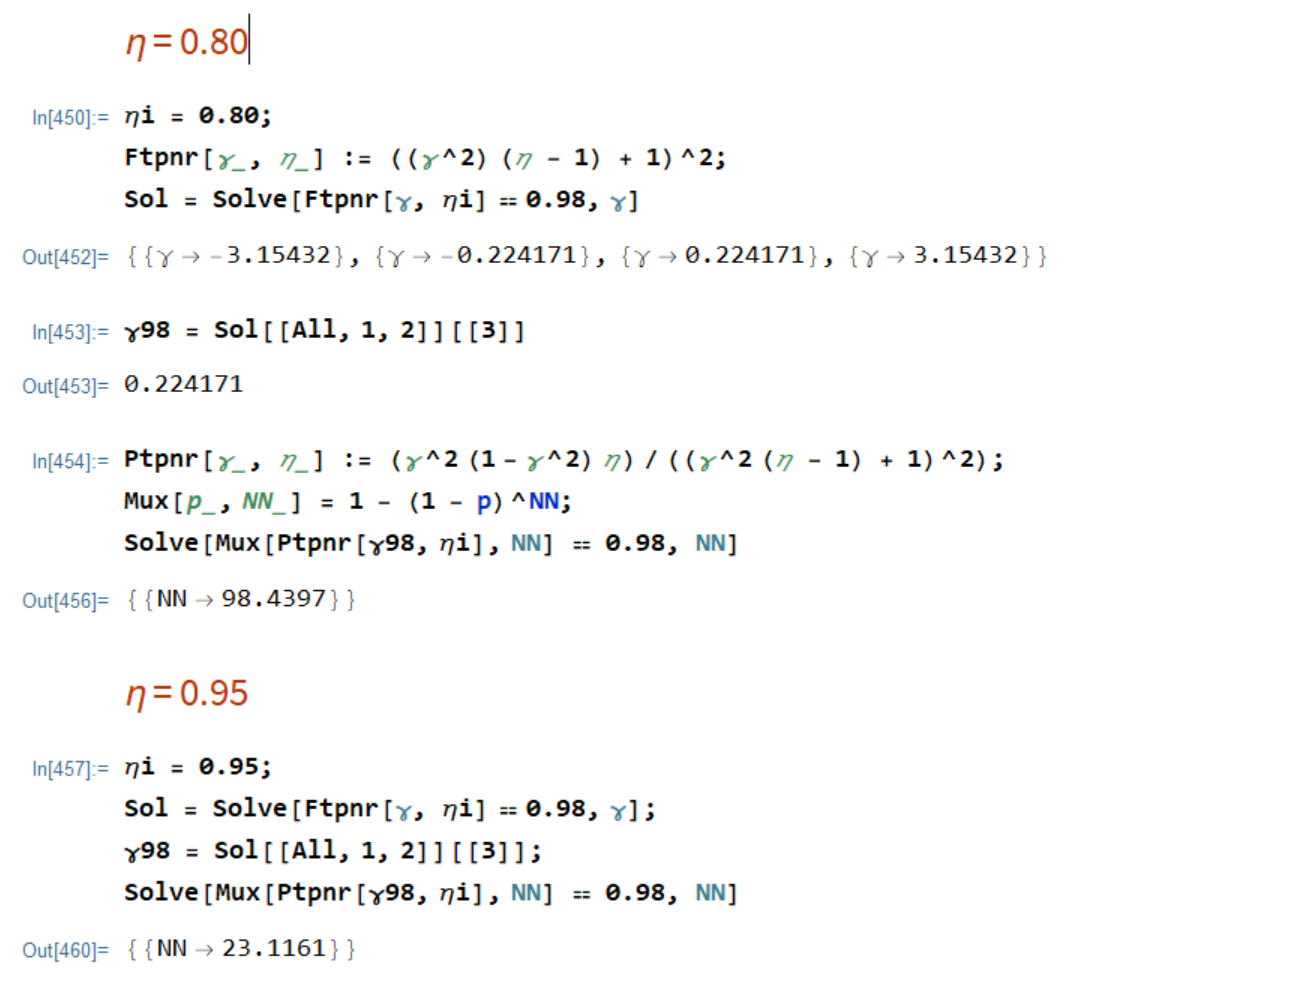
\includegraphics[width=0.7\textwidth,height=\textheight]{./chapter_07/figs/pnrTotalPerf.PNG}}

  \textcolor{midnightblue}{About $\boxed{\text{98 sources are needed for the case with an 80\% heralding}}$, }

  \textcolor{midnightblue}{about $\boxed{\text{23 sources are needed with 95\% efficient heralding}}$}

  \textcolor{darkred}{ 4 points for each of the 2 answers. Answers that vary from these values by 2-3 sources are acceptable. }
\end{enumerate}

\hypertarget{software-tools}{%
\chapter{Software Tools}\label{software-tools}}

\hypertarget{software-tools-for-equipment-and-experiment-control}{%
\section{Software Tools for Equipment and Experiment Control}\label{software-tools-for-equipment-and-experiment-control}}

Much of my time during the phd was spent writing software. While the main product of a phd is papers and the underlying ideas of the experiments carried out, software was often used to rigorously encode these more semantic or ephemeral results. Sometimes, the efficacy of a certain excremental idea depends greatly on the simplicity and reliability of the software used to implement it. If the setup of an initially complex excremental arrangement -- for example the synchronization of intensity modulators and arbitrary waveform generator with a mode locked laser -- can be made significantly more simple through the use of software, then the idea becomes more practical and more likely to be adopted by other researchers.

For these reasons I include introductions to the software tools on which I spent the most time and gained the most benefit. Perhaps these repositories provide insight that the thesis so far has not.

\hypertarget{sequence-generator}{%
\section{Sequence Generator}\label{sequence-generator}}

The Sequence Generator repository is for generating AWG sequences that are synchronized with the Pritel OAC fast mode locked laser. This is needed for carving the mode locked laser signal with intensity modulators. This toolset was useful for my PPM project as well as a concurrent high rate QKD project with slightly different requirements.

The most important feature of this toolset is the ability to determine compatible AWG sample rates and sequence lengths for a given laser repetition rate, while imposing certain requirements, like that the AWG sequence length must be a multiple of 128 samples. The script supports situations where a small integer number of laser pulses does not math in time an integer number of AWG samples. The main requirement is that the time for the full AWG sequence to run must be an integer multiple of the laser repetition period, so that the AWG sequence can be repeated indefinitely without drifting out of sync with the laser.

The sections of code that undergo this analysis are located in the functions \texttt{determine\_ppm\_properties} and \texttt{determine\_regular\_properties} for the PPM and QKD applications respectively.

\href{https://github.com/sansseriff/sequence_generator/tree/main}{Sequence Generator Repository}

\hypertarget{section}{%
\section{}\label{section}}

\hypertarget{software-systems-and-operation}{%
\section{Software Systems and Operation}\label{software-systems-and-operation}}

\hypertarget{advanced-matplotlib-layouts-with-the-bisect-function}{%
\subsection{\texorpdfstring{Advanced Matplotlib Layouts with the \texttt{bisect()} function}{Advanced Matplotlib Layouts with the bisect() function}}\label{advanced-matplotlib-layouts-with-the-bisect-function}}

It can be difficult to create complex plot layouts with matplotlib, especially when the layout should have strict requirements, like neighboring axes that are aligned with one another. Before explaining a custom method for solving this problem through the use of a new function \texttt{bisect()}, its worth reviewing the more accepted methods of advanced matplotlib figure layout.

\hypertarget{subplot-mosaic}{%
\subsubsection{Subplot Mosaic}\label{subplot-mosaic}}

\href{https://matplotlib.org/stable/gallery/subplots_axes_and_figures/mosaic.html}{Subplot mosaic} is a tool for specifying the layout of a figure with a special python dictionary, demonstrated by this example from the docs:

\begin{minted}
[
frame=lines,
framesep=2mm,
baselinestretch=1,
bgcolor=extralightgray,
fontsize=\footnotesize,
linenos]
{python}
fig = plt.figure(layout="constrained")
ax_dict = fig.subplot_mosaic(
    [
        ["bar", "plot"],
        ["hist", "image"],
    ],
)
ax_dict["bar"].bar(["a", "b", "c"], [5, 7, 9])
ax_dict["plot"].plot([1, 2, 3])
ax_dict["hist"].hist(hist_data)
ax_dict["image"].imshow([[1, 2], [2, 1]])
identify_axes(ax_dict)
\end{minted}

\includegraphics{./chapter_08/figs/sphx_glr_mosaic_001_2_0x.webp}

There are methods of changing the aspect ratios of the plots, but tools for imposing alignment constraints across plots are limited. For example, notice in the example above how the (1,1) plot axes are not vertically aligned with the (0,1) plot above.

\hypertarget{gridspec}{%
\subsubsection{Gridspec}\label{gridspec}}

\href{https://matplotlib.org/stable/gallery/lines_bars_and_markers/scatter_hist.html\#sphx-glr-gallery-lines-bars-and-markers-scatter-hist-py}{Gridspec} is a tool for more carefully specifying a grid layout. Space between plots can be specified, and the relative widths or heights of columns and rows can be customized. Gridspec offers a lot of control, but it requires many custom parameters that can be unintuitive to derive.

\hypertarget{add_axes}{%
\subsubsection{Add\_axes}\label{add_axes}}

One of the simplest ways of adding subplots to a figure is with the \texttt{fig.add\_axese(rect)} method. The \texttt{rect\ =\ {[}ll\_x,\ ll\_y,\ width,\ height{]}} specifies the x and y coordinate of the lower left corner with the first two parameters, and the width and height with the second 2 parameters. Multiple uses of \texttt{add\_axese()} offers maximum control for creating advanced layouts, but specifying all the correct \texttt{rect} arrays can get very confusing. Figure Fig.~\ref{fig:layout_sketch} illustrates the types of calculations that become necessary when the specific location and size of each subplot must be specified under certain constraints.

\hypertarget{fig:layout_sketch}{%
\begin{figure}
\centering
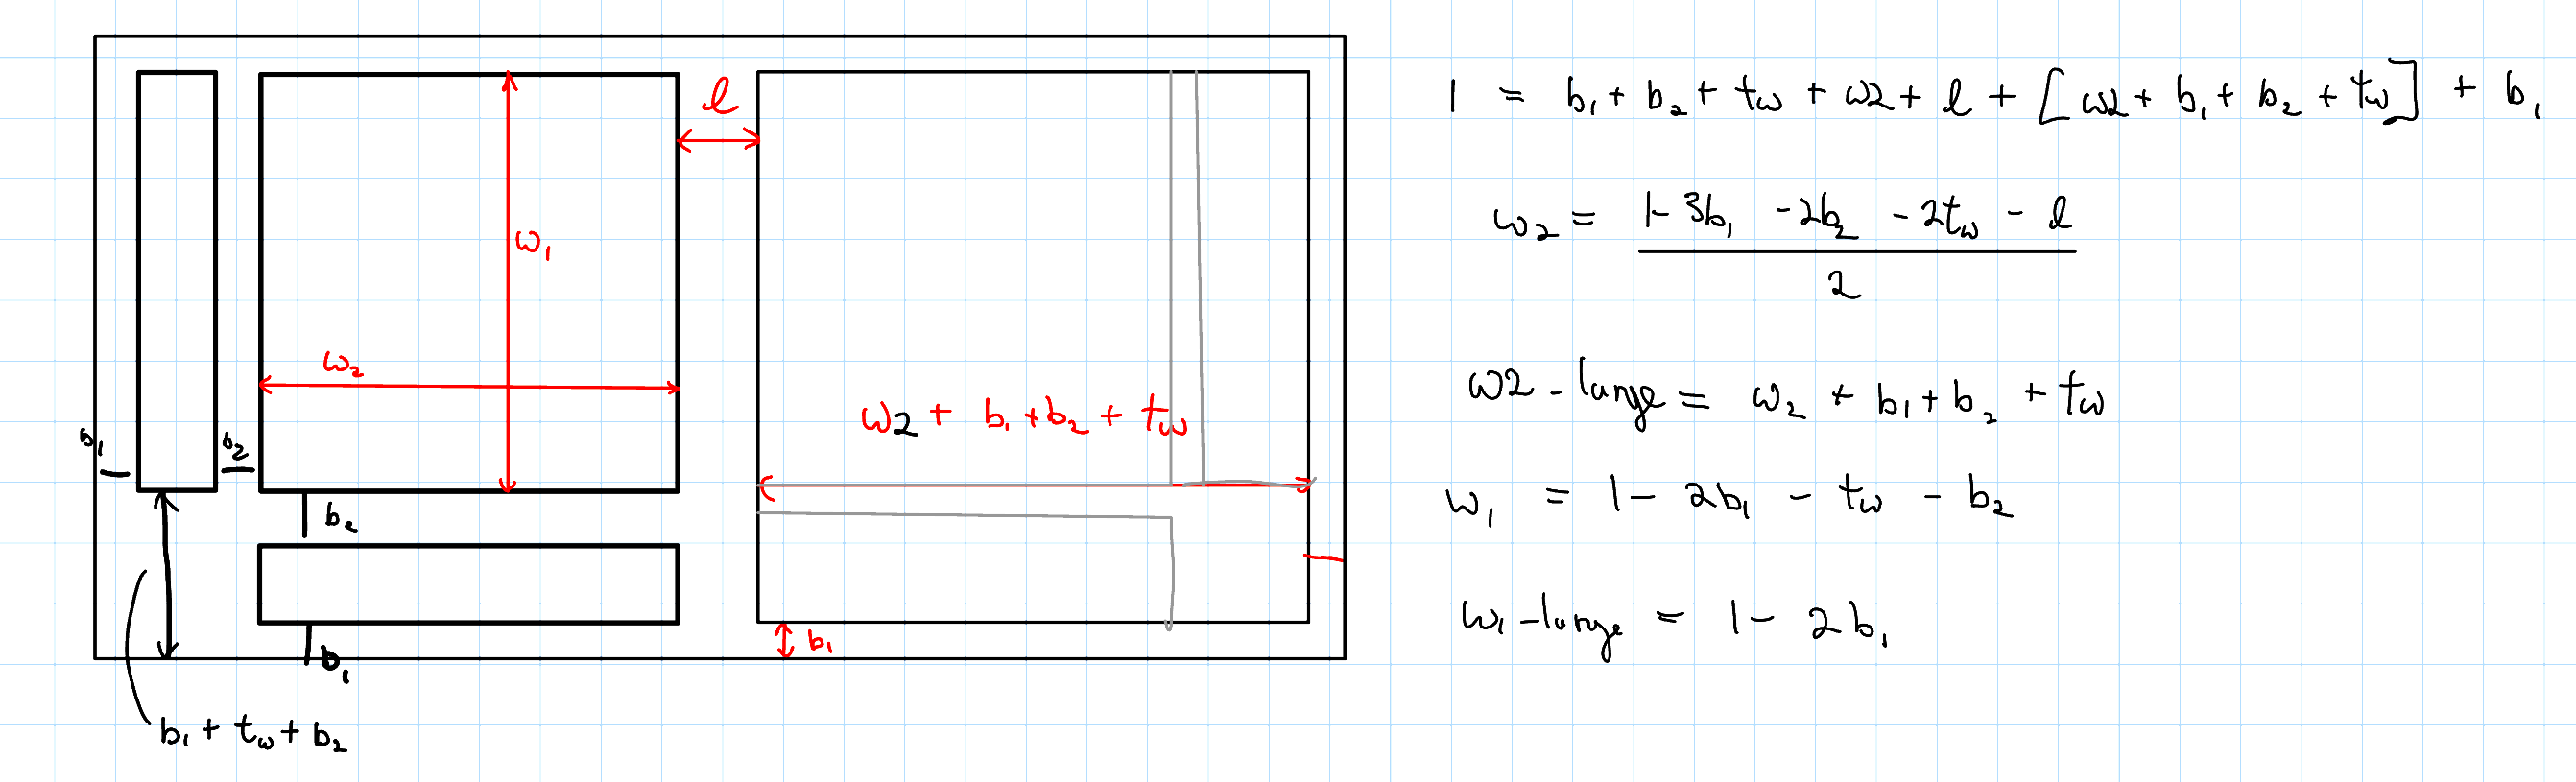
\includegraphics{./chapter_08/figs/layout_sketch.png}
\caption[{Rough sketch for layout with add\_axese()}]{\textbf{Sketch for layout with add\_axese().}}
\label{fig:layout_sketch}
\end{figure}
}

\hypertarget{bisect-method}{%
\subsubsection{\texorpdfstring{\texttt{bisect()} method}{bisect() method}}\label{bisect-method}}

\hypertarget{how-a-sorption-fridge-works}{%
\section{How A Sorption Fridge Works}\label{how-a-sorption-fridge-works}}

to put something only in the mkdocs/html output:

to put something only in the latex output:

to get numbered equations to work in both latex and html, use this format. Notice that the label is used twice, once inside the align block and once outside:

\hypertarget{eq:cosines}{}{ 
\begin{align}
P_{A+ B+} &= |\langle 2|2\rangle|^2_{A+ B+} = 2(1 + v \cos(\theta)) \label{eq:cosines}\\
P_{A+ B-} &= |\langle 2|2\rangle|^2_{A+ B-} = 2(1 - v \cos(\theta)) \notag \\
P_{A- B+} &= |\langle 2|2\rangle|^2_{A- B+} = 2(1 - v \cos(\theta)) \notag \\
P_{A- B-} &= |\langle 2|2\rangle|^2_{A- B-} = 2(1 + v \cos(\theta)) \notag \\ \notag
\end{align}
}

You can do footnotes like this\footnote{This is a footnote}

use \boldsymbol for bold latex:

\textbf{Fidelity and Rates vs $\boldsymbol \mu$}

Here are a few bold characters together: $\boldsymbol{\mu \quad \beta \quad \gamma}$

For units, use \mathrm{nm}:
This is a number with units: $138.3~\mathrm{nm}$

Refer to a figure with Fig.~\ref{fig:figurename} or Fig.~\ref{fig:figurename} or for multiple Fig.~\ref{fig:figurename}

Until I figure something more shorthand, you can set colors with ``\textless span\textgreater{}'' tags:

\textcolor{midnightblue}{ This text is blue. And it changes lightness when darkmode is witched }

\hypertarget{fig:figurename}{%
\begin{figure}
\centering
\includegraphics[width=0.7\textwidth,height=\textheight]{./chapter_08/figs_06/fig1b_light.pdf}
\caption[{Figure label for in thesis index here.}]{\textbf{Caption title here} a) Long caption here}
\label{fig:figurename}
\end{figure}
}

\hypertarget{fig:figurename2}{%
\begin{figure}
\centering
\includegraphics[width=0.7\textwidth,height=\textheight]{./chapter_08/figs_06/hsps_light.pdf}
\caption[{Figure label for in thesis index here.}]{\textbf{Caption title here} a) Long caption here}
\label{fig:figurename2}
\end{figure}
}

to have a ``~'' space in latex and a no break space in html\ldots{} ``\&\#160'', just use ``~''. That's a forward slash and a space.

The formatting of multi-line divs is very important. This will render correctly:

{\color{midnightblue} 

$$math stuff 1$$

}

But this won't:

{\color{midnightblue} 

\begin{minted}
[
frame=lines,
framesep=2mm,
baselinestretch=1,
bgcolor=extralightgray,
fontsize=\footnotesize,
linenos]
{nil}
$$math stuff 2$$
\end{minted}

}

And this won't

\begin{minted}
[
frame=lines,
framesep=2mm,
baselinestretch=1,
bgcolor=extralightgray,
fontsize=\footnotesize,
linenos]
{nil}
$$math stuff 3$$

</div>
\end{minted}

the file where you're working on bokeh styling is at :

C:\Users\Andrew\OneDrive - California Institute of Technology\JPL.Jitterate\peacoq\src\bokeh\_hists\_js\_callbacks.ipynb

\printbibliography
\end{document}
